%Documentclass thesul modifée pour la page de garde : thesul-cs
\documentclass[11pt]{thesul-cs}
\usepackage[utf8]{inputenc}
\usepackage[T1]{fontenc}
\usepackage{amsmath}
\usepackage{amsfonts}

%Fancy headers
\usepackage{fancyhdr}
\pagestyle{fancy}
\fancyhf{}
\fancyhead[LE,RO]{\thepage}
\fancyhead[LO]{\rightmark}
\fancyhead[RE]{\leftmark}

%mini table of contents
\usepackage[french]{minitoc}
\usepackage{amssymb}
\usepackage{xcolor} % où xcolor selon l'installation
\usepackage{mdframed}
\usepackage{multirow} %% Pour mettre un texte sur plusieurs rangées
\usepackage{multicol} %% Pour mettre un texte sur plusieurs colonnes
\usepackage{scrextend} %Forcer la 4eme  de couverture en page pair
\usepackage{tikz}
\usepackage{graphicx}
\usepackage[absolute]{textpos} 
\usepackage{colortbl}
\usepackage{amsmath}
\usepackage{amsthm}
\usepackage{stmaryrd}
\usepackage{array}
\usepackage{url}
\usepackage[ruled,french,frenchkw,onelanguage]{algorithm2e}
%\usepackage{algorithm}
%\usepackage{algpseudocode}
\SetAlCapSkip{1em}
\SetKwInput{KwInput}{Input}
\SetKwInput{KwOutput}{Output}
\usepackage{mathtools}
\DeclareMathOperator{\sign}{sgn}
\newtheorem{propriete}{Propriété}
\newtheorem{proposition}{Proposition}

%draft/release options
\newif\ifDraft
\newcommand\comment[1]{\ifDraft {\itshape\color{red}{#1}} \fi} %text displayed in draft mode as comments
\newcommand\draft[1]{\ifDraft #1 \fi} %text displayed in draft mode only.
\newif\ifReview
%switch between draftmode and releasemode
\ifdefined\draftmode
  \Drafttrue
  %\Reviewtrue
\fi

\ifdefined\reviewmode
  \Reviewtrue
\fi


%\Drafttrue %switch to false if you want to get the release version.
%\Draftfalse %switch to true if you want to get the draft version.
\ifReview \usepackage[lmargin=5cm]{geometry}\fi

%def path for files


%---------------------------
% (1) Weights
%---------------------------
\newcommand\w{\omega}

%---------------------------
% (2) External inputs
%---------------------------
\newcommand\inpx{X}

%---------------------------
% (3) Contextual inputs
%---------------------------

\newcommand\inpc{\gamma}

%---------------------------
% (4) Contextual suffix
%---------------------------
\newcommand\cont{_{c}}

%---------------------------
% (5) External suffix
%---------------------------

\newcommand\ext{_{e}}

%---------------------------
% (6) Map index
%---------------------------
\newcommand\m[1]{^{({#1})}}

%---------------------------
% (7) BMU
%---------------------------

\newcommand\bmu{\Pi}

%---------------------------
% (7) Neighborhood radius
%---------------------------
\newcommand\h{h}

\DeclareMathOperator*{\argmax}{arg\,max}


%compile only a chapter

\begin{document}
\dominitoc
\ThesisTitle{Auto-organisation Décentralisée Multi-Cartes}
\ThesisDate{ ? décembre 2022}
\ThesisAuthor{Noémie Gonnier}
\ThesisUL
% Jury:
\President = {Le président &du jury}
\Rapporteurs = {Le rapporteur 1 &du laboratoire\\
Le rapporteur 2\\
Le rapporteur 3}
\Examinateurs = {L’examinateur 1\\
L’examinateur 2}
\MakeThesisTitlePage
\tableofcontents
\section*{Introduction}



\subsection*{Bio-inspiration : une thématique actuelle}

Le terme calcul désigne les procédés abstraits utilisés pour le traitement de l'information. Un système réalisants de tels procédés est alors désigné comme système de calcul. D'un point de vue abstrait, ces systèmes peuvent être biologiques comme artificiels.
Aussi le cerveau humain est un système de calcul : il transforme une multitudes de signaux physiques et chimiques provenant des capteurs du corps humain en activité électrique qui se traduisent en des actions sur l'environnement. De nombreux systèmes biologiques sont ainsi des systèmes de calcul dans le sens ou ils traitent de l'information: cellules, organismes vivants ...
La majorité des systèmes de calculs artificiels développés actuellement ont d'ailleurs commencé par une inspiration biologique. En particulier, l'intelligence artificielle et le développement des systèmes d'apprentissage automatique ont comme point de départ la question des calculs réalisés biologiquement. Le modèle de neurone artificiel utilisé en deep learning s'appuie ainsi d'abord sur un modèle biologique de neurone.
Même si la diversité des applications actuelles de l'apprentissage automatique s'est éloignée de la compréhension biologique, la question des calculs occurants dans les systèmes biologique reste une thématique de recherche dans de nombreux domaines cherchant à simuler des comportements biologiques tels que les neurosciences computationnelles. 
Inversement, les systèmes  de calcul biologiques, par leur diversité de comportements encore incompris, restent une source d'inspiration majeure pour le développement de systèmes de calcul artificiels.

Nous nous intéressons dans cette thèse à une approche bio-inspirée de la conception de systèmes de calculs, en  particulier de systèmes d'apprentissage.
Un aspect récurrant, voire de fond observé en biologique est la modularité des systèmes. On peut définir la modularité d'un système comme sa composition en sous-systèmes autonomes effectuant des tâches différentes et collaborant entre eux. Cette modularité présente des aspects de réutilisation, de robustesse à des fautes, de traitement local de l'information. En soi, tout système peut être modulaire en fonction de la représentation qu'on lui choisit~; mais il existe des similitudes dans la structure de nombreux systèmes. De nombreux systèmes biologiques sont en effet composés de nombreux modules de même structure, ayant des règles d'évolution locales,  interagissant entre eux. Dans ce cas, le comportement global du système est plus.
Certains expliquent même le coté modulaire comme une conséquence de la sélection évolutive des systèmes.

 Les neurones du cerveau en sont un exemple. Chaque neurone est construit sur le même modèle et les règles d'évolution de chaque neurone sont similaires. Dans son ensemble, le cerveau présente des comportements de calculs qui lui sont propres.
Dans ce même cerveau, à  une plus grande échelle, on peut séparer des zones fonctionnelles distinctes dans le cerveau. Chaque zone est de construction similaire, mais effectue une fonction différente.
Le cerveau n'est pas le seul système biologique présentant ce type de fonctionnemment. Ainsi, les systèmes métaboliques ou d'expression de gènes sont des exemples de systèmes aggrégeant des éléments.
Les colonies de fourmi sont constituées de milliers d'individus effectuants des actions à leur échelle et communiquant localement. Le comportement de la colonie est un système de calcul, capable de résoudre des problème d'optimisation de chemin vers une source de nourriture.
Les calculs occurrant dans ces systèmes modulaires sont appelés comportements émergeant : chaque module du systèmes effectue des calculs et actions locales, mais le comportement du tout est plus complexe que la somme de chaque partie.
Cette notion d'émergence, dont nous avons donné des exemples biologiques, a inspiré de nombreux modèles de calcul en intelligence artificielle et robotique.
Par exemple, l'intelligence d'essaim (swarm intelligence) est une direct application de ce concept à des sytèmes multi-agents qui interagissent localement avec leur environnement. 
Le jeu de la vie permet d'effectuer des calculs et de propager de l'information malgré la simplicité des règles d'évolution de chaque cellule. Enfin, les calculs rendus possibles dans les réseaux de neurones proviennent du comportement collectif des neurones et sont donc un exemple d'émergence au sein de systèmes d'apprentissage.


La modularité présente des aspects avantageux pour le calcul, voire optimaux. En témoigne les architectures de modèles artificiels, a priori pas du tout inspirés de la biologie, à des modèles biologiques existants. Une structure de réseau en petit monde est  utilisée dans des systèmes d'information, comme des bases de données, comme une structure optimisant la vitesse des échanges d'information dans le système. Or, ces strctures sont observées dans de nombreux domaines expérimentaux : biologie (exemple ?) et même dans des systèmes sociaux tels que les arbres de connaissances entre individus.

 D'un point de vue informatique, on peut définir la modularité comme la décomposition d'un système en sous-systèmes plus petits et fonctionnant indépendamment. Ces systèmes interagissent via une interface bien définie.
Plusieurs façon de construire ces sous-systèmes. Dans un cas de figure, ces composants sont conçus pour être interchangeables et réutilisables.
La modularité permet alors à un système d'être robuste à un dysfonctionnement d'un composant, sa mise à l'échelle et un faculté d'adaptation.

Un système modulaire n‘est pas forcément un système complexe.
Cependant, lorsque l'interaction des modules est diverse et non linéaire, le système mène à l'émergence de nouveaux comportements.

\subsection*{Modularité et Conception d'architectures d'apprentissage}

Les systèmes d'apprentissage existants combinent la notion de modularité et d'émergence pour former des comportements d'apprentissage plus complexes.
Les réseaux de deep learning, se sont éloignés du modèle biologique du neurone pour ajouter des règles de calculs plus informatiques comme la backpropagation. Cependant l'approche modulaire est resté une constante dans le développement des réseaux utilisés actuellements comme le modèle teacher student et les réseaux de neurones adversarials qui combinent des réseaux performant chacun une sous-tâche par rapport à l'autre.

La conception de système modulaire d'apprentissage peut passer par deux approches. D'un coté, une approche “finale” dans laquelle la finalité, l'application du système est connue. La conception du sytèmes passe alors par la décomposition de l'objectif en sous-systèmes et sous-tâches de manière à définir des modules particuliers.
L'approche inverse serait l'approche constructive, dans laquelle nous disposons de modules permettant des comportements simples de calculs et les associons entre eux pour former un système modulaire. Il est difficile de connaître à l'avance le comportement final de ce type de sytème et son étude passe donc par la simulation.
Cette approche, si elle n'est pas la plus rapide en terme de résultats applicatifs, a l'avantage d'ouvrir la porte à des comportement d'apprentissages qui peuvent être inattendus. 

Exemples d'archi modulaires d'apprentissage ? ART, Reservoir

\subsection*{Le calcul local et décentralisé, une problématique actuelle des réseaux de neurones}

Modularité et calcul local sont des problématiques liées. De nos jours, la consommation energetique grandissante des  algorithmes de traitement de l'information  

3 – Les cartes auto-organisatrices comme choix de modules

Nous avons choisi dans cette thèse de s'intéresser à cette deuxième approche~: développer un système modulaire apprenant en associant des réseaux existants connus. Nous nous intéressons spécialement aux cartes auto-organisatrices.

Si nous revenons à un aspect biologique, les cartes auto-organisatrices sont, par leur comportement un modèle simplifié des aires cérébrales. Les travaux conduits dans notre équipes ces dernières années se sont attachés à construire des architectures modulaires complètement cellulaires. Nous cherchons dans cette thèse à s'inspirer de ces travaux mais en les passant à une échelle moins cellulaire, dans un cadre de simplification du modèle. Cette simplification nous permet une recherche plus facile et moins coûteuse de nouveaux comportements d'apprentissage, tout en restant déclinable si besoin en version cellulaire.
Dans un cadre d'architecture modulaire, 


\section{Contributions et plan}

Cette thèse cherche donc, dans un cadre bio-inspiré, à construire une architecture modulaire décentralisée de cartes auto-organisatrices. L'idée de cette approche est de rechercher des nouveaux comportements d'apprentissage émergeant de l'interaction entre les modules d'une grande architecture, à l'inverse des méthodes plus ingénieures consistant à diviser une tâche connue en sous-systèmes.
Nous commencerons par présenter un état de l'art des architectures de cartes auto-organisatrices existantes afin de définir ce qu'on entend par architecture modulaire décentralisée et positionner notre modèle dans l'ensemble des modèles existants.
Nous détaillerons ensuite notre modèle d'architecture décentralisée de cartes auto-organisatrices.
Si le modèle a pour but à long terme de concevoir une architecture comportant de nombreux modules, nous avons concentré cette thèse sur l'analyse des comportements d'architecture de deux et trois cartes.
Le but de cette thèse est alors de proposer une méthodologie d'analyse de ce modèle et d'en tirer des comportements élémentaires.
Nous proposerons une méthode expérimentale et des représentations rapprochant l'architecture de cartes de modèles d'apprentissage communs au chapitre 3.
Les résultats présentés dans les chapitres 4,5,6,7 présentent le comportement du modèle CxSOM sous différents angles.
Nous analyserons plus en détail l'interface entre cartes et une recherche de BMU originale que nous utilisons.
Nous présenterons ensuite les comportements élémentaires observés sur des architectures de deux et trois cartes en une dimension, qui sont plus facile à visualiser. Nous présenterons notamment un comportement de prédiction rendu possible par le modèle.
Nous proposons au chapitre 6 des indicateurs numériques originaux d'évaluation de l'apprentissage associatif par l'architecture de cartes, dans le but d'étendre l'analyse du modèle à des architectures difficilement représentables visuellement.
Le chapitre 7 applique la méthode d'observation à des cartes en deux dimensions afin de saisir la scalabilité du modèle.

Les travaux présentés dans cette thèse ont fait l'objet de deux présentations en conférence~:
\begin{itemize}
    \item Consensus driven ...., ICONIP 2020
    \item Input prediction in SOMs, ISCMI 2021
\end{itemize}

A placer : 

Apprentissage supervisé / non supervisé définition.
Mémoire associative/traitement de séquences 


% \begin{itemize}
%     \item Apprentissage non supervisé, quantification vectorielle : définition + apprentissage développemental ? Pq c'est cool de continuer a etudier les SOM ?
%     \item Modularité et modularité dans les programmes informatiques,définition
%     \item Systèmes dynamiques complexes~: Biologique first puis exemple automates cellulaires qui sont une machine de turing, réseaux de Hopfields, machine de bolztmann: comporements de calcul comme émergeance
%     \item Systèmes d'apprentissage modulaire : des systèmes complexe.
% \end{itemize}

% \cite{Oudeyer2010OnTI} : biologie liée dans les deux sens à l'aspect computationnel.


% But : montrer comment un mécanisme de recherche de consensus entre cartes de Kohonen permet de construire des architectures apprenant des relations multimodales.
\mainmatter
\documentclass[../main]{subfiles}
\ifSubfilesClassLoaded{
    \dominitoc
    \tableofcontentsfile
}{}
\begin{document}

\graphicspath{{01-Modularite/},{./}}
%%%%%%%%%%%%%%%%%%%%%%%%%
% Intro du chapitre : Trouver un questionnement, un exemple qui parle de modularité dans les systèmes biologiques:  
% se placer dans le contexte de 
% - modularité : finalement on ne sait pas trop ce que c'est 
% - apprentissage ! 
% - réseaux de neurones
%%%%%%%%%%%%%%%%%%%%%%%%%
\chapter*{Introduction}


Le terme d’intelligence artificielle apparaît en 1956 lors d’une conférence donnée à l’université de Dartmouth, Dartmouth Summer Research Project on Artificial Intelligence. Cette conférence rassemble des chercheurs issus de différents domaines en plein essor de création comme la cybernétique, le traitement de l’information, la logique, la biologie, et veut poser les bases d’un nouveau domaine, nommé à cette occasion par les organisateurs Minsky et McCarthy: “Intelligence artificielle”. 

Ce terme générique est en fait large: on va appeler intelligence artificielle tout programme capable d’effectuer des tâches compliquées dont seuls les humains étaient initialement capables de résoudre. 
En terme d’architectures, les programmes d’intelligence artificielle peuvent être des systèmes figés à base de logique tels que les systèmes experts, ou des systèmes évolutifs. Parmi les tâches dites humaines se trouve en effet la notion d’apprentissage. La création  d’un système apprenant à partir d’entrées devient alors un enjeu à part entière de l’intelligence artificielle qu’on nommera apprentissage automatique ou en anglais machine learning.
Ces 60 dernières années ont alors vu les systèmes “intelligents” évoluer, se diversifier, pour résoudre de plus en plus de tâches jusqu’alors considérées comme humaines.

La conception de ces programmes passe par différentes sources d'inspirations, la biologie y prenant une place de premier choix.

\section*{Conception d'algorithmes d'apprentissage par modularité}

\subsection*{Définition de modularité}

La modularité en informatique se définit comme l'assemblage d'éléments séparés en une fonction globale, avec la condition qu'ajouter ou enlever un element ne modifie pas les autres éléments et influe seulement sur la fonction globale.

La majorité, voir tous les systèmes biologiques peuvent etre compris comme des systèmes modulaires. Il semble d'ailleurs que les systèmes modulaires sont privilégiés par l'évolution et des réseaux de forme similaire se retrouvent ainsi dans de nombreuses branches de la biologie: le cerveau présente des structures de réseau en petit monde que l'on retrouve dans l'organisation des ….
L'ingénieurie, sans même s'inspirer de la nature a recréé ces réseaux: les réseaux small world sont les plus efficaces pour la représentation de bases de données, ou la conception des réseaux aériens.
	
Cette notion de modularité concerne l'informatique en général: le concept peut etre appliqué au développement d'algorithmes.


\subsection*{Conception d'algorithmes d'IA}

La conception d'algorithme passe par piocher dans un ensemble de concepts et de fonctions connues, en les assemblant entre elles. 
La démarche de création d'algorithme peuvent etre ascendantes ou descendantes. 

Exemple d'algos d'IA → 
Ainsi, dans les années 1960, des premiers programmes d'intelligence artificielle repose sur des “micro mondes”, postulant qu'il est plus simple de décomposer les taches en taches plus simples afin de résoudre des comportements plus compliqués.

\subsection*{Approche ascendante vs approche descendantes}

On peut choisir deux axes de recherche pour développer un programme modulaire.
 L'approche descendante, la plus souvent utilisée, part du problème applicatif à résoudre pour le décomposer en probèmes-blocs plus simples.  et on estime que l'assemblage d'éléments exécutant ces fonctions simples nous permettrons d'effectuer la fonction complexe.
Cette démarche est très applicative. Elle est maitrisée: on connait la fonction finale, il suffit de trouver les meilleurs composants pour effectuer cette tache. Généralement, on a de bons résultats
Par contre, on ne pourra pas trouver de nouveaux paradigmes de calculs dans ce cadre: il s’agit plutot d’utiliser et d”appliquer des méthodes connues. 

Dans une démarche ascendante, il s’agit de partir de fonctions simples qu’on assemble dans l’idée d’en créer des complexes. Cette démarche est plutot exploratoire : la complexité du système fait que le seul moyen de comprendre le comportement du système ainsi créé est de le simuler. Cela peut etre vu comme un désavantage: pas possible d’avoir des équations et de choisir correctement les paramètres sans une étude des simulations. L’avantage par contre est de laisser de nombreuses opportunités ouvertes pour de nouvelles formes de calcul.
Et c’est précisément ce point qui nous amène à nous placer dans une telle démarche dans cette thèse. Nous voulons trouver de nouvelles formes de calcul pour faire de l’apprentissage. 

-----

\section*{ Modularité, systèmes complexes et emergence}

Un autre axe motivant notre reflexion sur des architectures modulaires d’apprentissage est l’observation que les systèmes modulaires sont des systèmes complexes. 

\subsection*{Système modulaire = système complexe ? }

Un système complexe est un système dont l'état est décrit par un certain nombre de variables qui évoluent de façon non linéaire. → def de qui ?
Dans la littérature, on rencontre également cette définition: système composé d'un grand nombre d'élements connectés entre eux. Cette définition rejoint la première, mais on peut noter qu'un système peut etre complexe meme à partir de 3 variables, tel que le modèle climatique de Lorentz ou le pendule triple.
 
La complexité d'un système est plutot un mode de représentation du système. La notion de systèmes complexes a été introduite dans les années 70 (Lorenz), et connait un essor depuis l'avenement des calculateur performants. 

Théorie des réseaux complexes

\subsection*{Emergence de calcul au sein d'un système complexe}

On va caractériser l'émergence de comportement dans un système complexe comme “le tout est plus que la somme des parties”, c'est à dire qu'on ne peut pas comprendre un système en le décomposant en éléments et en analysant chaque élémént individuellement: il va falloir considérer les relations entre éléments. 
La notion de systèmes complexe est étroitement liée à celle d'auto-organisation. La présence de patterns réguliers dans le comportement d'un système est directement liée à sa complexité.

\subsection*{Emergence de calcul comme moyen de conception de nouveaux algo d'IA}

D'un point de vue de création de systèmes, cela veut dire qu'on peut construire un système a partir d’éléments séparés, dont le comportement global résulte de l'interaction de ces éléments..
Le deep learning a été construit a partir du perceptron comme un assemblage de couches, dans le but de ????



\section*{ Plan de la thèse}

Dans cette thèse, nous voulons prendre une démarche constructive d'un algorithme d'apprentissage afin d'explorer de nouveaux paradigmes de calcul. Nous explorerons donc un système modulaire donc les modules sont des structures d'apprentissage existantes. Ce modèle dynamique est un système complexe, duquel pourra émerger des comportements
L'émergence de phénomènes d'auto organisation au sein des systèmes complexe nous pousse a considérer des modules possèdant déjà cette capacité d'auto-organisation: les cartes auto-organisatrices de Kohonen.
Le but de cette thèse est ainsi, dans une démarche constructive, de rechercher des nouveaux comportement d'apprentissage  à partir de cartes de Kohenen ,assemblées en architectures.
Nous nous intéressons à des modèles décentralisés, étant la clé pour construire n'importe quel type d'architecture par la suite. 
Cette démarche est difficile dans la mesure ou le comportement final d'une architecture n'est pas prédictible de prime abord. Tout l'exercice de cette thèse est alors de construire un modèle et définir des règles d'interaction, puis simuler et analyser ce modèle pour en tirer des comportements émergeants participant à l'apprentissage.
Dans cette démarche de construction, nous avons choisi des contraintes:
- Nous réalisons un système modulaire de cartes auto-organisatrices
- Cette architecture sera décentralisée: nous voulons permettre aux modules de communiquer avec n'importe lequel des autres éléments.
Le problème de cette thèse est d'étudier les comportements émergent de tels systèmes et d'étudier comment ces comportements sont un apprentissage des données.
Nous comparerons dans un premier chapitre les systèmes de cartes auto-organisatrices présentes dans la littérature et positionnerons l'architecture que nous développerons dans ce manuscrit au regard des travaux existants. Ces travaux nous permetterons de poser des hypothèses concernant le comportement qu'on peut attendre de l'architecture que nous développons. Nous présenterons ensuite le modèle CxSOM.
Nous définirons dans un chapitre la démarche expérimentale utilisée pour évaluer l'architecture de cartes et la représenter. Enfin, nous montrerons des comportements de base emergeant de la structure que nous avons développée et montrerons qu'elle a un capacité de mémoire associative. Nous présenterons egalement les limites du modèle. 
A l'issue du manuscrit, nous souhaitons que le lecteur aie une compréhension des comportements de base du modèle proposé, et aie des pistes pour l'utiliser de façon plus applicative.
\begin{figure}
    \begin{minipage}{0.49\textwidth}
        
\includegraphics[width=\textwidth]{220px-Giant_Pufferfish_skin_pattern_detail}
    \end{minipage}
    \begin{minipage}{0.49\textwidth}
        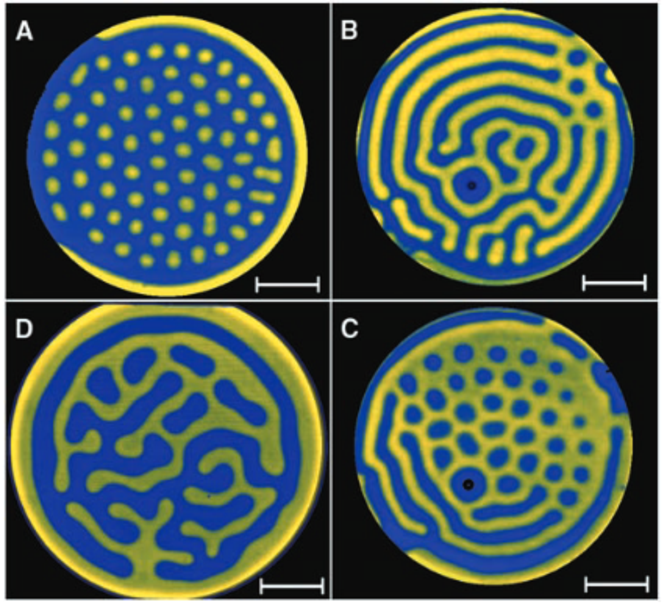
\includegraphics[width=\textwidth]{turing_pattern_chem.pdf}
    \end{minipage}
\end{figure}
\end{document}








\chapter{Modèle d'architecture CxSOM}
\graphicspath{{02-SOM/}}
\minitoc

Nous proposons dans cette thèse un modèle d'architecture de cartes auto-organisatrices, CxSOM. Par ce modèle, on associe des cartes auto-organisatrices en architecture afin de réaliser des tâches de mémoire associative: apprendre un modèle de relation entre des ensembles de données issues de plusieurs modalités. 
On souhaite que ce modèle soit générique, permette de construire n'importe quel forme et taille d'architecture, et aie la possibilité d'intégrer des connexions récurrentes. Notre démarche est d'abord de proposer un nouveau modèle de calcul général à base de cartes auto-organisatrices; des applications plus spécifiques pourront être développées à partir de cette méthode. Nous avons publié le modèle CxSOM en~\cite{gonnier2020}.


On définit une \emph{architecture} de carte par un réseau composé de plusieurs modules qui sont chacun des cartes de Kohonen et dans lequel des connexions sont définies entre ces modules. Ces connexions sont orientées: on parle d'une connexion d'une carte A vers une carte B. Le but de ces connexions est de coupler l'apprentissage de plusieurs cartes.
Sur une telle architecture, on peut construire un graphe $G$ orienté, dont les n\oe{}uds sont des cartes. La connexion d'une carte A vers une carte B est indiquée par la présence d'une arête de A vers B. On appelle architecture \emph{non-hiérarchique} une architecture pour laquelle le graphe $G$ n'est pas un arbre: il présente des boucles. Un exemple d'architecture non-hiérarchique est par exemple représenté en figure~\ref{fig:archi_non_hierarchique}. Certaines cartes sont connectées dans les deux directions, d'autres en boucle. Dans cette thèse, nous chercherons à utiliser de telles architectures non-hiérarchiques pour des tâches de mémoire associative.
Ici, chaque carte de l'architecture cherche à apprendre une représentation d'une des entrées $A,B,C,D,E$ qui lui est fournie. 
Lorsque ces entrées sont dépendantes les unes des autres, l'architecture dans sa globalité doit également, d'une façon ou d'une autre extraire les relations, les dépendances, existant entre les distributions de données. Cet apprentissage de relations est au c\oe{}ur de cette thèse et sera détaillé dans le chapitre d'analyse de l'architecture.

Dans ce chapitre, nous détaillons d'abord le modèle CxSOM développé et étudié durant cette thèse, permettant de construire des architectures non-hiérarchiques de cartes auto-organisatrices. Nous présentons en premier lieu le formalisme d'une carte de Kohonen classique, dont sont dérivées les cartes auto-organisatrices utilisées dans les architectures CxSOM. Nous expliquerons ensuite les choix de développement sur lesquels nous nous sommes appuyés pour développer le modèle. Nous présenterons le modèle sur un exemple d'architecture à deux cartes, puis nous le formaliserons pour le cas général de $n$ cartes connectées au sein d'une architecture. Le glossaire des notations est fourni en annexe.

\begin{figure}
\centering
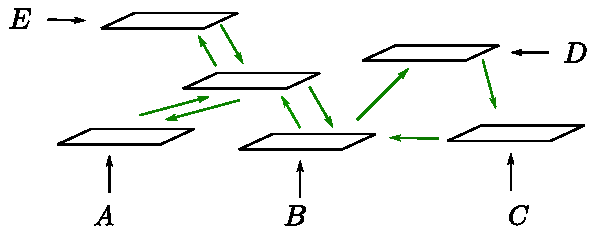
\includegraphics[width=0.6\textwidth]{architecture.pdf}
\caption{Deux exemples d'architectures \emph{non-hiérarchiques} à 3 cartes de Kohonen: des connexions sont réciproques, ou des boucles sont présentes au sein de l'architecture.
Les entrées sont $A,B,C,D,E,F$ quelconques.}
\label{fig:archi_non_hierarchique}
\end{figure}


\section{Carte de Kohonen classique}\label{sec:kohonen}
Chaque carte de Kohonen d'une architecture CxSOM est directement dérivée de l'algorithme d'une carte de Kohonen classique introduite en \cite{Kohonen1982}, et décrite extensivement par Kohonen en \cite{Kohonen1995SelfOrganizingM}. Le principe général d'une carte de Kohonen a été décrit dans le chapitre précédent; nous définissons ici plus précisément le modèle et les équations qui serviront de base pour la définition de l'algorithme CxSOM.

\subsection{Algorithme et notations}
Une carte de Kohonen est un graphe, généralement une ligne 1D ou une grille 2D de $N$ n\oe{}uds. Nous utiliserons dans cette thèse des cartes en une et deux dimensions, c'est à dire des lignes et des grilles. Les notations et le modèle présentés ici sont toutefois applicables à des cartes de dimensions et topologie quelconques.

L'algorithme et les notations sont résumés en figure~\ref{fig:one_map_not}. Une entrées fournie à une carte de Kohonen est notée $\inpx_t$, tirée dans un espace d'entrée $\mathcal{D}$. A chaque n\oe{}ud de la carte est associé un poids, appelé aussi prototype, noté $\w_e \in D$. Sa \emph{position} dans la carte est indexée par $p$. Nous choisissons d'indexer les positions entre $0$ et $1$: l'ensemble des positions $p$ est donc un ensemble de points discrets entre $0$ et $1$. L'ensemble des poids est noté $\{\w_e(p), p \in \{0,\cdots,\frac{i}{N}, \cdots, 1\}\}$, avec $i$ l'indice entier d'un noeud de la carte. On peut faire la même discrétisation de l'espace pour une carte en 2D.

Une étape $t$ de l'algorithme de mise à jour d'une carte de Kohonen contient les étapes suivantes:
\begin{enumerate}
\item\label{enum:inp} Une entrée $\inpx_t$ est tirée et présentée à la carte.
\item\label{enum:act} Une \emph{activité} $a_e(\inpx_t,p)$ est calculée dans la carte pour chaque noeud de position $p$. La fonction d'activité choisie est gaussienne:
\begin{equation}\label{eq:act1som}
a_e(\inpx_t,p) = \exp{\frac{\lVert \inpx_t-\w\ext(p) \rVert ^2}{2\sigma^2}}
\end{equation}
\item\label{enum:bmu} L'unité ayant l'activité maximale est la \emph{Best Matching Unit} de la carte. Sa position est notée $\bmu$. Cette étape est déjà une modification de l'algorithme original de Kohonen.
Dans la version classique, on calcule plutôt les distances entre l'entrée et les poids $\lVert \inpx_t - \w_e(p) \rVert$, et le BMU est choisi comme l'unité dont le poids présente la plus petite distance à l'entrée. 
Ici, on prendra comme BMU l'unité ayant l'activité la plus élevée.
\item Chaque poids $\w_e$ est déplacé vers l'entrée $\inpx$. Le déplacement est pondéré par une \emph{fonction de voisinage} $H(\bmu,p)$. Cette fonction est maximale en $p = \bmu$ et décroissante autour de cette position. Dans notre étude, la fonction de voisinage est triangulaire, donc maximale en $\bmu$, décroissante sur un \emph{rayon de voisinage} noté $h_e$ et nulle sinon.
\begin{equation}
\w_e(p,t+1) = \w_e(p,t) + \alpha H(\bmu,p)(\inpx_t - \w_e(p,t))
\label{eq:update}
\end{equation}
\end{enumerate}


\begin{figure}
\centering
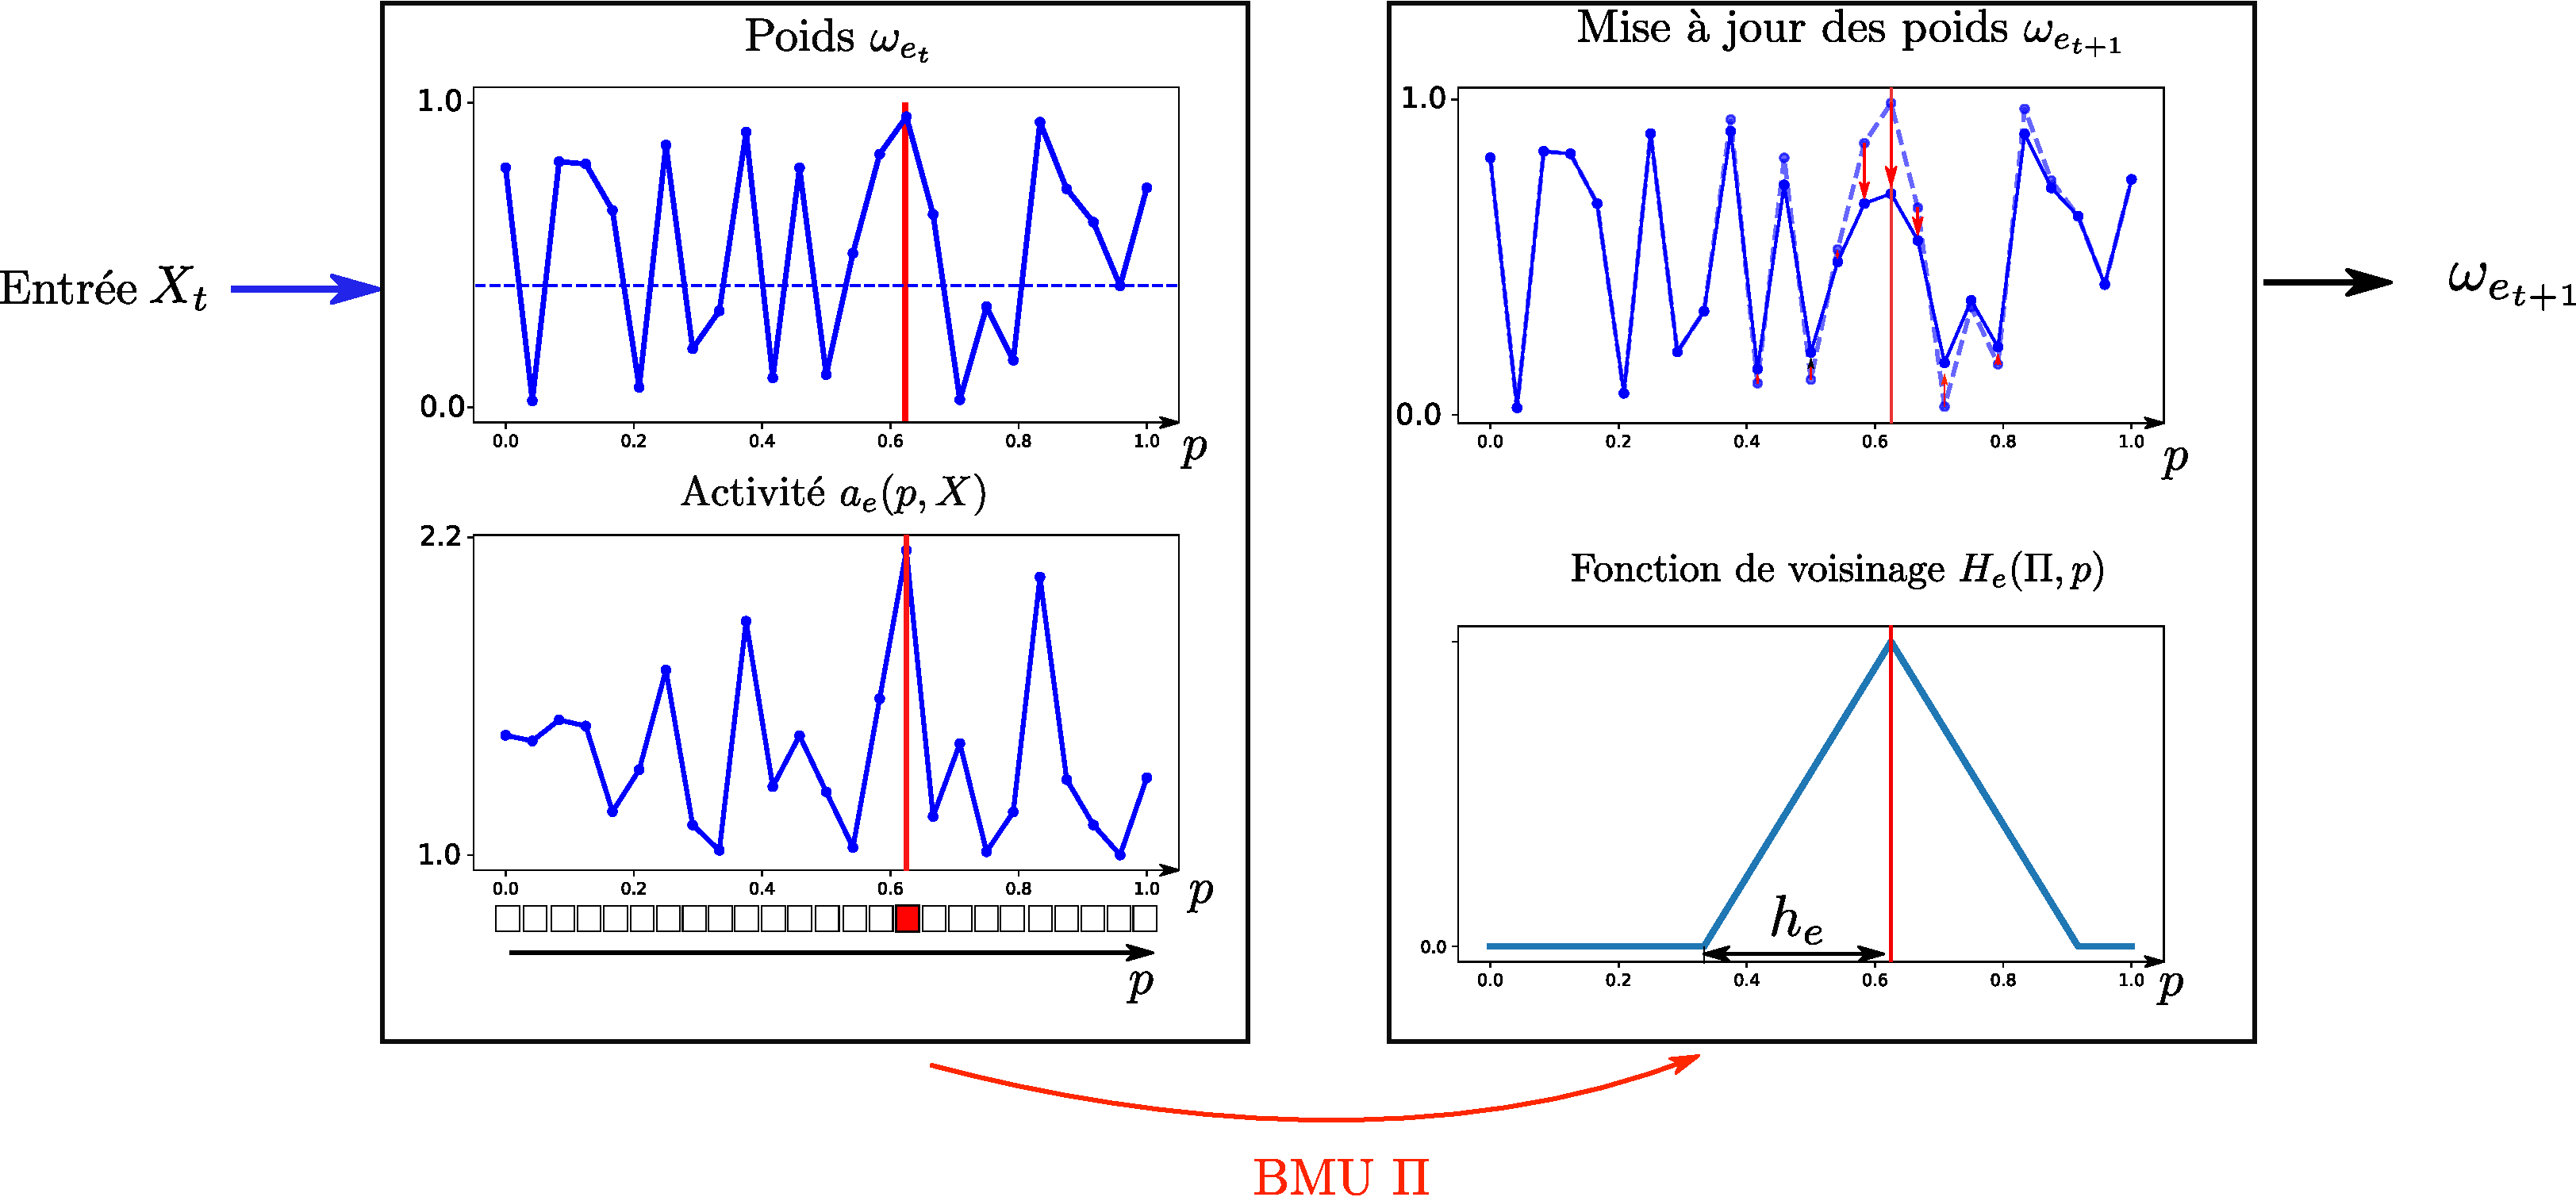
\includegraphics[width=\textwidth]{one_map_one_layer2.pdf}
\caption{Notations utilisées dans une carte de Kohonen simple. Les 4 étapes d'une itération d'apprentissage sont présentées: 1. Présentation de l'entrée, 2. Calcul de l'activité, 3. Choix du BMU, 4. Mise à jour des poids.}
\label{fig:one_map_not}
\end{figure}


\subsection{Paramètrage d'une carte de Kohonen}
L'organisation d'une carte de Kohonen est gérée par plusieurs paramètres. 
Nous détaillons ici les choix de paramètres effectués. Les paramètres supplémentaires introduits par la version CxSOM seront présentés plus tard en partie \ref{sec:params}.

\subsubsection{Taux d'apprentissage $\alpha$}
Le taux d'apprentissage $\alpha$ détermine la proportion dans laquelle chaque poids est déplacé vers l'entrée lors de sa mise à jour, selon l'équation~\ref{eq:update}. Dans l'algorithme classique, le taux d'apprentissage décroît au cours de l'apprentissage. Au début de l'apprentissage, $\alpha$ est élevé, ce qui assure un dépliement rapide de la carte. $\alpha$ est ensuite diminué manuellement tout au long de l'apprentissage. Cette décroissance assure la convergence des poids de la carte au cours de l'apprentissage.

Un objectif à long terme de développement de l'architecture CxSOM est de développer des systèmes de cartes autonomes, intégrant le traitement de données séquentielles. Dans ce cas d'utilisation, il n'est pas souhaitable de faire décroître le taux d'apprentissage qui introduit un début et une fin d'apprentissage fixés par avance. Le calcul d'une itération dépend alors non seulement de l'état précédent de la carte, mais aussi de l'itération $t$ courante.
Dans une logique de développement futur, nous utiliserons un taux d'apprentissage constant au cours des itérations dans CxSOM. Les calculs réalisés lors d'une itération $t$ dépendent alors uniquement de l'état précédent.


\subsubsection{Topologie de la carte}

Le graphe supportant la carte de Kohonen peut présenter diverses formes, comme détaillé en section~\ref{sec:som001}: grilles, lignes, arbres, graphes ... Les notations et l'algorithme CxSOM que nous présentons dans ce chapitre sont applicables à toutes les formes de cartes. Les expériences et l'évaluation du modèle se concentrent quant à elles sur des lignes 1D et des grilles 2D, et omettent les formes de graphes quelconques. Ce choix est d'abord motivé par le fait que les lignes et les grilles sont les formats de cartes les plus courants rencontrés dans la littérature. On parle souvent de cartes de Kohonen 1D et cartes 2D, en sous-entendant le format de ligne ou de grille du graphe support. 


Ensuite, la spécificité des cartes de Kohonen tient à l'organisation des prototypes de façon continue. Lorsqu'on parle de continuité des prototypes dans une carte de Kohonen, il s'agit d'abord d'une relation de proximité et d'ordre entre des prototypes discrets: \emph{si deux unités sont proches dans la carte, alors leurs prototypes sont proches dans l'espace d'entrée}. Un exemple d'organisation des poids d'une SOM en ligne 1D sur des données dans $[0,1]$ est tracé en figure~\ref{fig:depliement}. Les prototypes sont répartis aléatoirement dans l'espace d'entrée $[0,1]$ à l'itération $0$; au cours de l'apprentissage, ils s'organisent de façon ordonnée. A partir de l'itération 500, on observe cette continuité des prototypes.

Le format particulier de ligne et de grille d'une carte de Kohonen permet d'étendre cette notion de proximité entre prototypes à une continuité des poids au sens mathématique, par interpolation. Dans ces formats 1D et 2D, l'ensemble des n\oe{}uds et leurs arêtes est inclus dans une ligne ou un plan: chaque arête peut être vue comme un ensemble de positions. Les poids de la carte sont dans ce cas une approximation discrète d'une fonction continue $\widetilde{\w_e}$, à valeurs dans~$\mathcal{D}$.
\begin{equation*}
\begin{array}{ccccc}
M& : & [0,1]^2 \; \text{ou} \;[0,1] & \to &  \mathcal{D} \\
 & & p & \mapsto & \widetilde{\w_e}(p) \\
\end{array}
\end{equation*}

Cette continuité est une des puissances d'une carte de Kohonen en tant qu'algorithme de quantification vectorielle. Des opérations réalisées dans l'espace des positions $[0,1]$ correspondent directement à des opérations dans l'espace d'entrée $\mathcal{D}$, par la fonction $\widetilde{\w_e}$.

Au cours de l'apprentissage, les poids d'une carte se rapprochent de la distribution des données. On parlera de \emph{dépliement} d'une carte pour parler de son apprentissage.
Pour une carte 1D sur des données 1D, il est démontré en \cite{Kohonen1995SelfOrganizingM} que les poids évolueront au cours de l'apprentissage vers un ordre strictement croissant ou strictement décroissant; ordre qui ne sera plus modifié une fois atteint. 
Lorsque la dimension des données est plus grande que celle de la carte, par exemple des points 2D ou des images (256 dimensions), la carte formera des plis de manière à remplir l'espace $\mathcal{D}$ (voir figure~\ref{fig:som1d}, section~\ref{sec:som001}). 

\begin{figure}
\centering
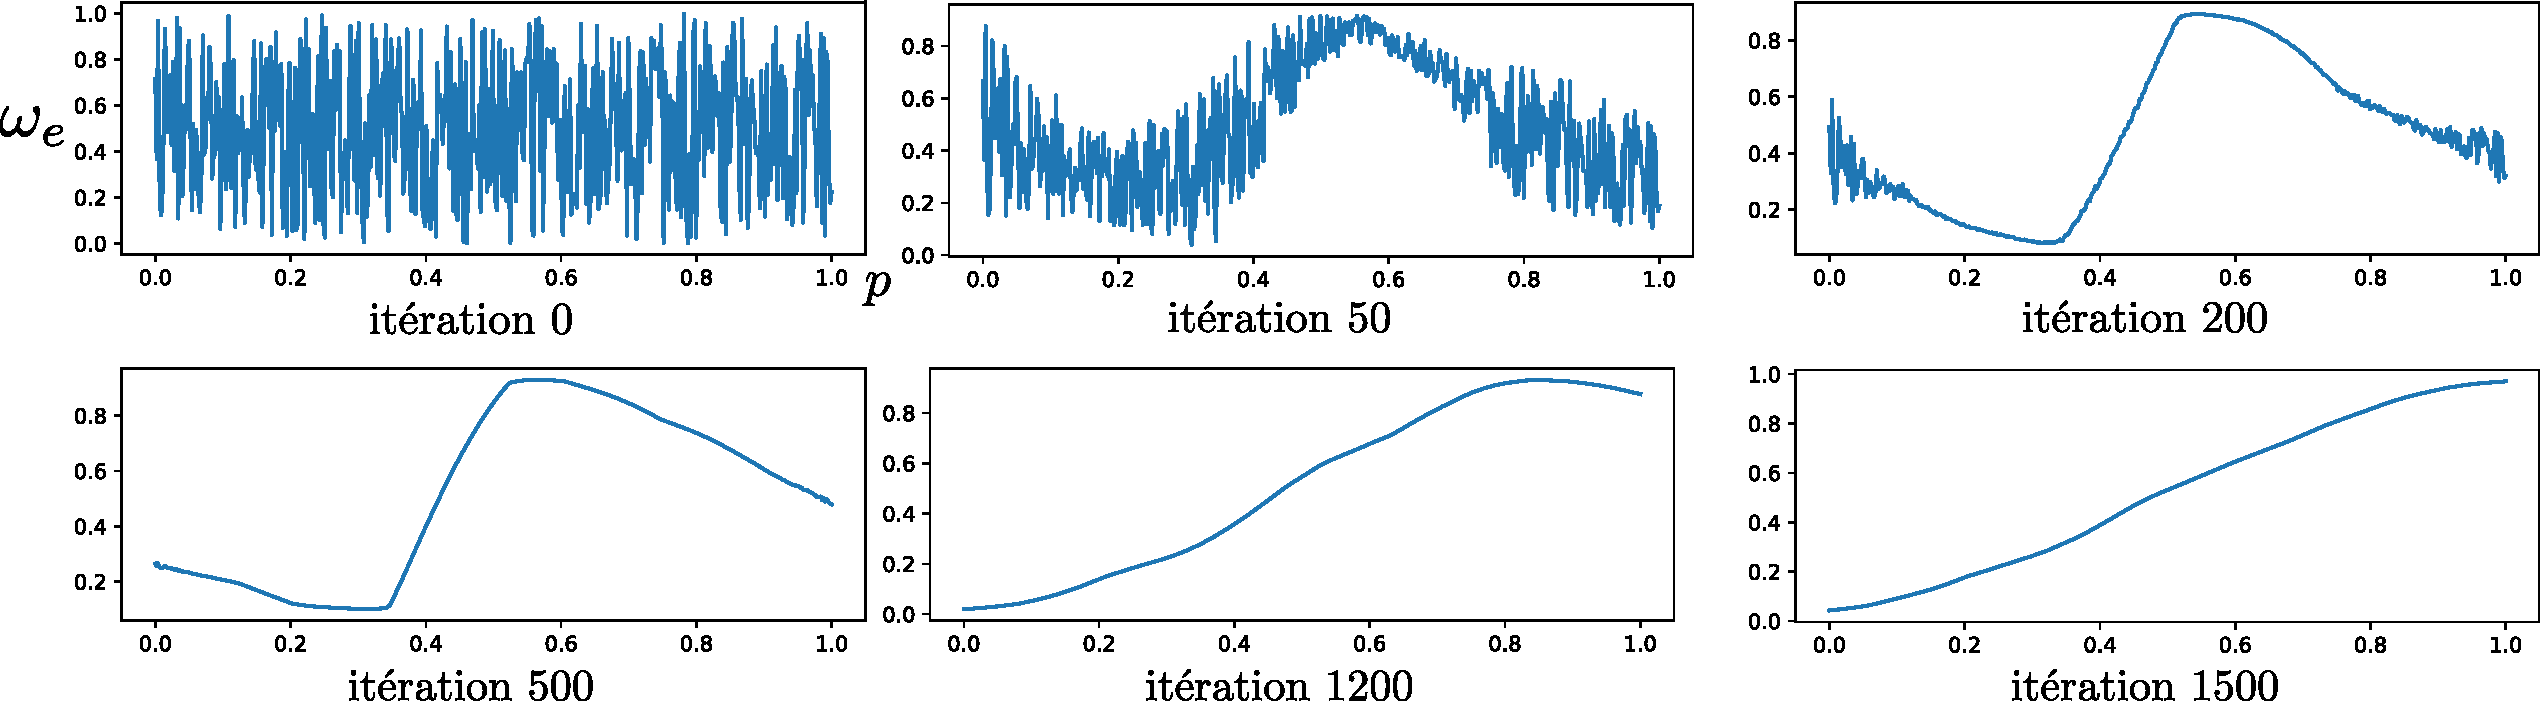
\includegraphics[width=\textwidth]{depliement_1D.pdf}
\caption{Exemple de dépliement d'une carte 1D de taille 500, sur des données 1D $\inpx \in [0,1]$. Les paramètres $h\ext = 0.2, \: \alpha = 0.2$ ont été gardés constants dans cet exemple. On s'attend à ce que les poids de la carte soient organisés selon un ordre strictement croissant ou décroissant à la fin de l'apprentissage.}
\label{fig:depliement}
\end{figure}

\subsubsection{Rayon de voisinage}
Le choix de la fonction de voisinage est déterminant dans la topologie de la carte. Elle dépend en particulier du rayon de voisinage $h_e$.
Cette valeur détermine quelles unités voisines du BMU auront leurs poids mis à jour.
Plus le rayon $h_e$ est grand, plus la partie de la carte déplacée vers l'entrée lors de la mise à jour est étendue. 
Le rayon de voisinage détermine \emph{l'élasticité} d'une carte. Une carte ayant un grand rayon de voisinage est moins sensible aux variations locales des données et parvient à se déplier selon les variations à grande échelle de la distribution des entrées.
Un petit rayon d'apprentissage permet au contraire de déplacer les poids concentrés dans une petite région sans affecter toute la carte. Les poids s'ajustent ainsi aux variations locales des entrées. Par contre, choisir un rayon de voisinage petit au début de l'apprentissage empêche la carte de se déplier globalement de façon ordonnée; au contraire, on verra apparaître des portions distinctes de cartes s'organisant de façon discontinue.
Le choix de l'élasticité est donc un compromis entre apprentissage d'une structure globale des entrées et ajustement aux variations locales.
Dans l'algorithme classique, ce compromis est trouvé en faisant décroitre le rayon de voisinage au cours de l'apprentissage. Un grand rayon de voisinage permet à la carte de se déplier rapidement en apprenant une structure globale des données. Sa décroissance au cours des itérations permet d'affiner l'apprentissage des données à un niveau plus fin. 
Contrairement à la plupart des SOM classiques, nous garderons des rayons de voisinage constants dans CxSOM. Tout comme le fait de garder le taux d'apprentissage constant, garder le rayon de voisinage constant est motivé par les objectifs de traitement de données séquentielles.

\section{Motivations du modèle CxSOM}
A partir du modèle de carte de Kohonen détaillé en section \ref{sec:kohonen}, nous proposons une version de carte auto-organisatrice servant de bloc de base pour construire des architectures non-hiérarchique de cartes. L'idée de construire une telle architecture est de traiter plusieurs ensembles de données de façon jointe, pour réaliser de la mémoire associative.
Nous présentons tout d'abord les choix de développement effectués pour créer le modèle d'architecture.

\subsection{Champ d'application: mémoire associative}
L'architecture CxSOM a pour but de développer une mémoire \emph{associative} au sein d'une architecture de cartes. On considère donc un ensemble d'espaces $\mathcal{D}\m{1}, \cdots , \mathcal{D}\m{n}$, différentes \emph{modalités} sur lesquelles on effectura de la quantification vectorielle. Les entrées présentées à une architecture de cartes sont $(\inpx\m{1}, \cdots, \inpx\m{n}) \in \mathcal{D}\m{1} \times \cdots \times \mathcal{D}\m{n}$. Pour pouvoir développer une mémoire associative, on se place dans des cas où les modalités considérées ne sont pas indépendantes les unes des autres: les distributions marginales $\inpx\m{i}$ ne sont pas indépendantes. La tâche de mémoire associative cherche alors à extraire des schémas de dépendance entre modalités. Lorsqu'on tire une entrée pour la présenter à une carte, on tire une entrée jointe $\mathbf{\inpx} =  (\inpx\m{1}, \cdots , \inpx\m{n})$, puis chaque composante est présentée à la carte qui lui correspond. Pour respecter l'homogénéité des entrées necessaires à l'apprentissage d'une carte auto-organisatrice, on normalise les espaces $\mathcal{D}\m{i}$ pour que toutes les entrées soient à valeur dans $[0,1]^k$, $k$ la dimension de $\mathcal{D}\m{i}$.

Dans les exemples de cette thèse, on tire des entrées jointes en 3 dimensions, donc chaque composante 1D est présentée à une carte. Chaque modalité est la coordonnée sur un des axes du point 3D tiré. Nous utiliserons par exemple, en tant qu'espace dont les modalités sont dépendantes, un ensemble de points sur un cercle en une dimension dans un espace en trois dimensions. Chaque coordonnée $X$, $Y$, $Z$ dépend alors des deux autres coordonnées. On évaluera comment l'architecture que nous présentons dans cette partie apprend les données mais surtout leurs relations. 

Les exemples porteront sur des modalités en une dimension, mais les dimensions de chaque modalité peuvent être quelconque.
\begin{figure}
\centering

\includegraphics[width=\textwidth]{inputs_3som}
\caption{Exemple de disposition d'entrées. Les modalités associées à différentes cartes sont les coordonnées $x,y,z$ de chaque point. Dans une telle disposition, les modalités dépendent les unes des autres: développer une mémoire associative signifie apprendre le modèle de relation existant etre $x,y$ et $z$, c'est à dire le cercle.}
\label{fig:inputs}
\end{figure}

\subsection{Description de l'architecture}

Nous avons vu au chapitre précédent la notion de contexte transmis entre cartes. Dans CxSOM, on choisit de se placer dans le paradigme de transmission de la position du BMU entre cartes: on connecte une carte B à une carte A en donnant la position du BMU de B en entrée à la carte A. 
Ce paradigme de partage de positions rappelle à la fois le modèle hiérarchique HSOM~\cite{lampinen_clustering_1992}, et les modèles de cartes récurrentes s'appuyant sur SOMSD \cite{hammer_recursive_2004,hagenbuchner_self-organizing_2003,fix20}.


Contrairement aux cartes hiérarchiques HSOM dans lesquelle la position du BMU est la seule entrée d'une carte de plus haut niveau, chaque carte de l'architecture peut posséder une entrée principale propre issue d'une modalité $\inpx\m{i}$, l'entrée \emph{externe}. L'entrée ou les entrées correspondant aux positions des BMUs d'autres cartes sont considérées comme une entrées supplémentaires d'une carte. Les cartes auto-organisatrices dans le modèle CxSOM prennent donc un nombre arbitraire d'entrées, dont certaines sont les BMUs d'autres cartes. On appelle ces entrées internes à l'architecture les entrées \emph{contextuelles} d'une carte.
L'algorithme d'apprentissage d'une carte auto-organisatrice prenant une position de BMU en tant que contexte est similaire à celui d'une carte classique, comprenant:
\begin{enumerate}
\item\label{etape:entree} Présentation de son entrée à la carte 
\item\label{etape:bmu} Recherche du BMU par calcul d'activité
\item\label{etape:maj} Mise à jour des poids selon une fonction de voisinage
\end{enumerate}

Chaque carte aura maintenant plusieurs entrées: une entrée \emph{externe} dans un espace d'entrée, et $k$ entrées \emph{contextuelles} qui sont les positions des BMUs des cartes qui lui sont connectées. La carte peut aussi ne pas prendre d'entrée externe, seulement des entrées contextuelles.
La recherche du BMU doit être modifiée par rapport à la méthode originale : les rétroactions entre les cartes sont autorisées, la position du BMU de la carte A va donc influencer la position du BMU de la carte B, lequel modifie à nouveau le BMU de la carte A, etc. 

Notre algorithme implémentera deux modifications principales par rapport à l'algorithme d'apprentissage d'une carte de Kohonen classique: 
\begin{itemize}
\item Les cartes possèdent plusieurs entrées, externes et contextuelles; les entrées contextuelles sont les positions des BMUs d'autres cartes. Le calcul de l'activité est modifié afin de prendre en compte ces différentes couches d'entrées.
\item La recherche du BMU est modifiée afin de gérer les rétroactions entre cartes.
\end{itemize}

L'architecture CxSOM couple ainsi l'apprentissage de plusieurs cartes. Elles apprennent à la fois sur leurs données $\inpx\m{i}$, mais contextualisées selon les informations issues des autres cartes. Notons que les cartes apprennnent de façon jointe dès le début de leur apprentissage. Seule la position du BMU est utilisée comme information transmise entre carte. Cette valeur a l'avantage d'apporter une homogénéité dans l'architecture de cartes: quelles que soient les entrées d'une carte et leurs dimensions, le BMU sera une position en 1 ou 2 dimensions. Si on prenait le poids du BMU comme valeur transmise, par exemple, comme peut le faire la carte récurrente MSOM~\cite{Strickert2005MergeSF}, l'information circulant entre les cartes dépendrait des dimensions des entrées.
De plus, transmettre seulement le BMU est une avantage en terme de quantité d'information à transmettre. Certains modèles, tel que le modèle de carte récurrente \cite{Voegtlin2002RecursiveSM} transmettent l'activité complète d'une carte en contexte. Certes, cette information reste indépendante du type d'entrée, est complète, mais lourde. La transmission du seul BMU, on le verra dans le chapitre d'analyse, est suffisante pour permettre l'apprentissage du modèle de relations entre données, qui est ce qu'on recherche avec les entrées multimodales. 

On laisse aussi la possibilité d'utiliser des cartes ne prenant que des entrées contextuelles. Ces cartes agissent alors comme des cartes intermédaires, connectant des cartes prenant des entrées externes.

L'algorithme CxSOM est détaillé en algorithme~\ref{algo:cxsom}; les parties suivantes expliquent et illustrent le modèle. Nous présentons d'abord le modèle sur un exemple de deux cartes, puis le formalisme étendu dans un cadre général d'architecture.

\section{Présentation de CxSOM: exemple d'une architecture de deux cartes}

Avant de présenter le modèle général de CxSOM sur une architecture quelconque, présentons le fonctionnement de l'architecture la plus simple qui soit: deux cartes $M\m{1}$ et $M\m{2}$, connectées réciproquement, présentée en figure~\ref{fig:2som_archi}. Toutes les équations seront formalisées dans le cas général en section~\ref{sec:formalisme}. 
On prend dans cet exemple des cartes en une dimension, indexées par $p \in [0,1]$. Les étapes sont d'abord détaillées, puis résumées en deuxième sous-partie.

\subsection{Détail des étapes}
\paragraph{Structure des cartes}
La carte $M\m{1}$ prend une entrée externe notée $\inpx\m{1}$ et une entrée contextuelle qui est le BMU de la carte $M\m{2}$ $\bmu\m{2}$. Les entrées externes $\inpx\m{1}$ et $\inpx\m{2}$ sont deux modalités interdépendantes; dans cet exemple, il s'agit des coordonnées $x$ et $y$ d'un point sur un cercle tel que présenté en figure~\ref{fig:inputs}. Les entrées externes sont donc également en une dimension.
La structure de chaque carte de l'architecture est adaptée à partir du modèle classique de SOM pour prendre deux entrées au lieu d'une. On indicera les élements des cartes par $(1)$ et $(2)$ pour désigner les éléments appartenant à la carte $M\m{1}$ et $M\m{2}$.
Une carte possède ainsi deux couches de poids: les poids \emph{externes} $\w_e\m{i}$, $i=1,2$ qui se déplient sur les entrées $\inpx\m{(i)}$, et les poids contextuels $w_c\m{i}$, qui se déplient sur l'espace des positions en une dimension de l'autre carte. Ces deux couches de poids sont représentées en figure~\ref{fig:2som_weights}. La position du BMU de $M\m{2}$, $\bmu\m{2}$ est utilisée comme entrée contextuelle de $M\m{1}$, et $\bmu\m{1}$ comme entrée contextuelle de $M\m{2}$. Les deux cartes apprennnent donc de façon couplée.

\paragraph{Calcul d'activité}
L'activité de la carte $a_g$ résulte de la combinaison entre l'activité \emph{externe} et l'activité \emph{contextuelle}. Ces deux activités sont calculées comme dans le modèle classique, équation~\ref{eq:act1som} et tracées en figure~\ref{fig:2som_activite}; l'activité externe compare les poids externes à l'entrée externe $\inpx_t$, et l'activité contextuelle les poids contextuels à l'entrée contextuelle.

Pour la carte $M\m{1}$, au pas de temps $t$, on a:
\begin{equation}
\label{eq:activite}
\begin{cases}
a_e\m{1}(\inpx_t\m{1},p) = \exp\frac{-\lVert \w_e\m{1}(p)-\inpx\m{1}_t \rVert^2}{2\sigma^2} \\
a_c\m{1}(\bmu\m{2},p) = \exp\frac{-\lVert \w_c\m{1}(p)-\bmu\m{2} \rVert ^2}{2\sigma^2}\\
\end{cases}
\end{equation}
$a_c$ et $a_e$ sont combinées en une activité globale:
\begin{equation}
a_g\m{1}(\inpx\m{1},\bmu\m{1},\bmu\m{2},p) = \sqrt{a_e(\inpx_t,p)\times \frac{a_e(\inpx_t,p) + a_c(\bmu\m{2},p)}{2}}
\end{equation}
Par la différence de contribution de $a_c$ et $a_e$ au sein de l'activité globale -- $a_c$ ne contribue qu'à la puissance $\frac{1}{2}$ -- on assure que l'activité contextuelle vient seulement moduler l'activité externe.
On peut observer cette modulation sur la courbe noire de la figure~\ref{fig:2som_activite}: l'activité globale suit la même progression que l'activité externe, mais est localement modifiée par les variations de l'activité contextuelle. De cette façon, les entrées contextuelles ne viennent pas donner d'hallucinations à la carte: elle apprend en priorité ses entrées externes, conditionnées aux entrées contextuelles. Cette façon d'assembler les entrées est inspirée des travaux conduits en \cite{menard_model_2005}.
Dans ces travaux, les auteurs combinent des activités par leur moyenne géométrique. 
Le sens de la moyenne géométrique est une sorte de "et" entre les activités, ce qu'on recherche ici aussi.
\begin{figure}
\centering
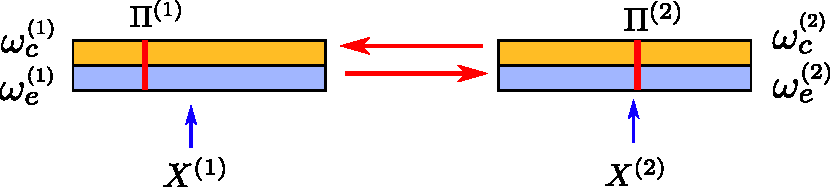
\includegraphics[width=0.7\textwidth]{archi_2som}
\caption{Architecture la plus simple possible de deux cartes. Le BMU $\bmu\m{1}$ de la carte $M\m{1}$ est utilisé en entrée de $M\m{2}$, et le BMU $\bmu\m{2}$ de $M\m{2}$ en entrée de $M\m{1}$. Chaque carte possède donc deux couches de poids. \label{fig:2som_archi}}
\end{figure}
\begin{figure}
\centering
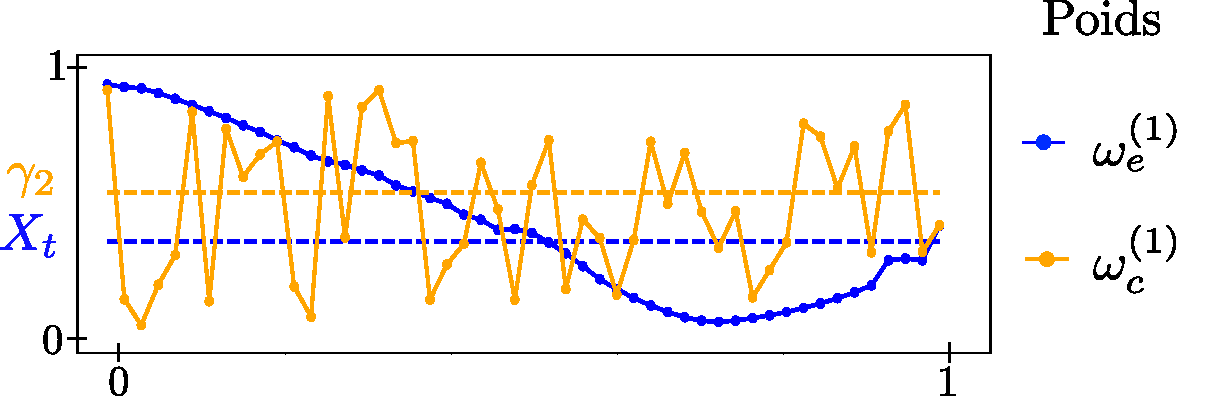
\includegraphics[width=0.75\textwidth]{weights_2som.pdf}
\caption{Représentation des poids de $M\m{1}$. L'entrée externe $\inpx_t$ présentée à l'itération $t$, tirée d'un espace d'entrée 1D $[0,1]$, est indiquée en bleu sur le graphique. L'entrée contextuelle  est le BMU de la carte $M\m{2}$. Sa valeur est indiquée en jaune; il s'agit d'une position 1D dans la carte $M\m{2}$, à valeur entre 0 et 1. La configuration des poids présentée dans cet exemple est atteinte durant le processus d'apprentissage de deux cartes $M\m{1}$ et $M\m{2}$, dont les entrées $\inpx\m{1}$ et $\inpx\m{2}$ sont les coordonnées de points tirés sur un cercle. \label{fig:2som_weights}}
\end{figure}
\paragraph{Relaxation}
Le calcul de $\bmu\m{1}$ dépend donc de $\bmu\m{2}$ et inversement. Contrairement à une carte simple, on ne peut pas calculer tous les BMUs de l'architecture un par un en prenant $\hat{p}$, l'argmax de $a_g$, comme BMU dans chaque carte.
On remplace l'étape de simple calcul d'argmax par un processus global à l'architecture de recherche de BMU. Cette recherche est réalisée par un processus dynamique que l'on appelera \emph{relaxation}, menant à un \emph{consensus} entre cartes : on cherche un point, s'il en existe, où le BMU de chaque carte est au plus proche du maximum de son activité globale $\hat{p}$.

Cette recherche est une boucle imbriquée dans un pas d'apprentissage $t$, indexée par $\tau$ et appelée relaxation. On définit une suite de BMUs intermédaires, $(\bmu\m{1}_\tau , \bmu\m{2}_\tau)$, $\tau$ variant de $0$ à un nombre d'itérations maximum $\tau_{max}$ fixé pour assurer une fin de la boucle. Le processus de relaxation est le suivant:
\begin{enumerate}
\item Les entrées externes sont présentées au début de la boucle, donc $a_e$ peut être calculée; $\bmu\m{1}_0$ et $\bmu\m{2}_0$ sont initialisées à la position où les activités externes sont maximales dans chaque carte. 
\item Tant que la suite de positions $(\bmu\m{1}_\tau,\bmu\m{2}_\tau)$ n'a pas convergé:
	\begin{enumerate}
	\item Dans chaque carte, calculer les activités contextuelles et globales, définissant ainsi $\hat{p}\m{1}_\tau = \argmax_{p\m{1}}(a_g\m{1}(p\m{1},\inpx\m{1}, \bmu\m{2})$, de même pour $\hat{p}\m{2}$.
	\item Déplacer $\bmu\m{1}$ vers $\hat{p}\m{1}$ et $\bmu\m{2}$ vers $\hat{p}\m{2}$ d'un pas $\Delta$: $\bmu\m{1}_{\tau+1} = \bmu\m{1}_{\tau} \pm \Delta$.
	Si une des valeurs est plus proche de $\hat{p}$ que $\Delta$, on déplacera $\bmu$ directement sur $\hat{p}$ pour éviter les oscillations autour du point. Cette étape est illustrée en figure~\ref{fig:relax}.
	\end{enumerate}
\item Le BMU de chaque carte est pris comme la valeur finale stable de ce processus dynamique. On note cette position finale $\bmu\m{i}_t$, désignant que cette valeur correspond à l'itération d'apprentissage $t$. Cette valeur est utilisée pour les mise a jour des poids. Si la relaxation n'atteint pas de point stable, on fixe tout de même un nombre d'itérations maximum après lequel on arrête la relaxation.
\end{enumerate}
\paragraph{Mise à jour}
Enfin, chaque couche de poids $\w\ext\m{i}$, $\w_c\m{i}$ est mise à jour indépendamment dans chaque carte relativement au BMU $\bmu\m{i}_t$ et les entrées externes $\inpx\m{i}_t$ et contextuelles $\bmu\m{j}_t$. Cette mise à jour correspond à la figure~\ref{fig:maj}. Les rayons d'apprentissage diffèrent entre couche externe et couche contextuelle.

\begin{figure}
\centering
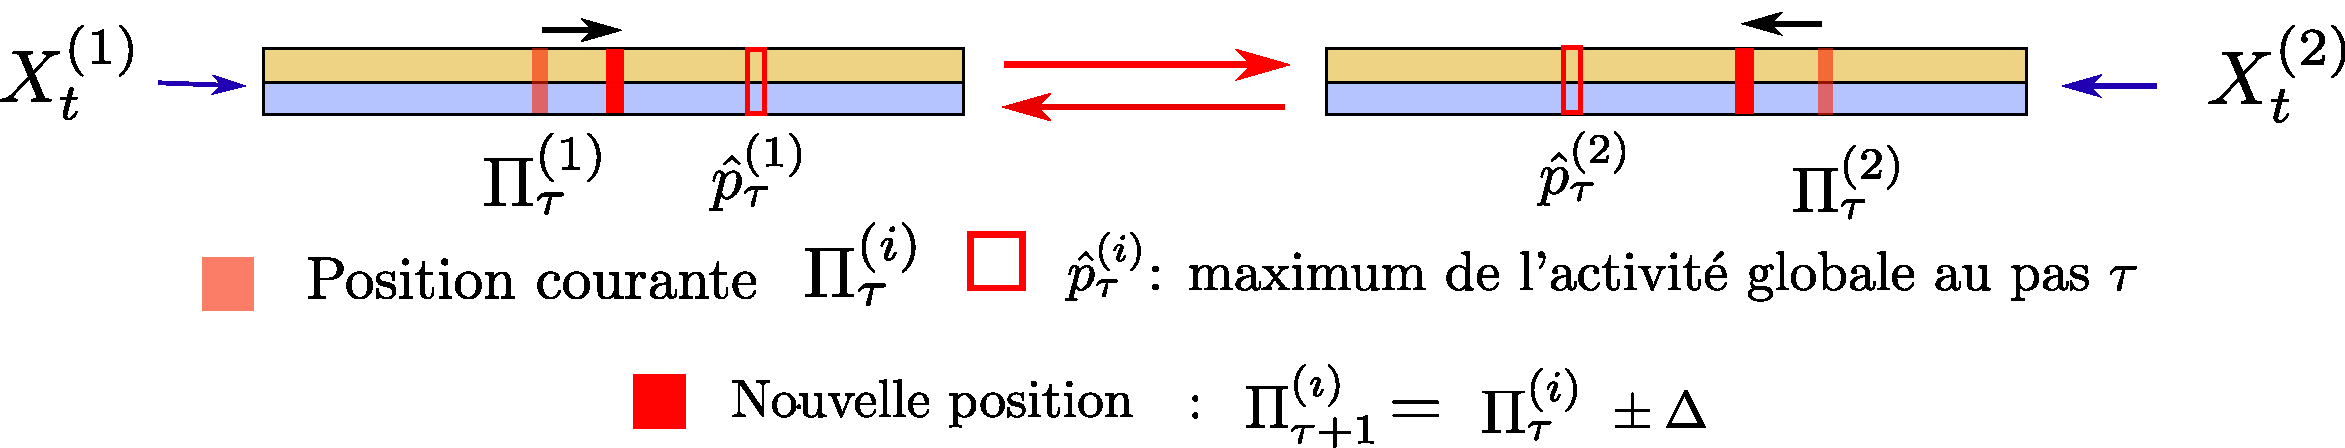
\includegraphics[width=\textwidth]{relaxation_2maps.pdf}
\caption{description d'une étape de la relaxation dans l'architecture, aboutissant à un consensus entre cartes. Au sein d'une même itération $t$, les position des BMU $\bmu$ sont légèrement déplacées jusqu'à ce que toutes les positions $\bmu$ des cartes de l'architecture soient stable. Ces positions maximisent collectivement les activités globales de chaque carte. \label{fig:relax}}
\end{figure}

\begin{figure}
%\begin{minipage}{0.6\textwidth}
\centering
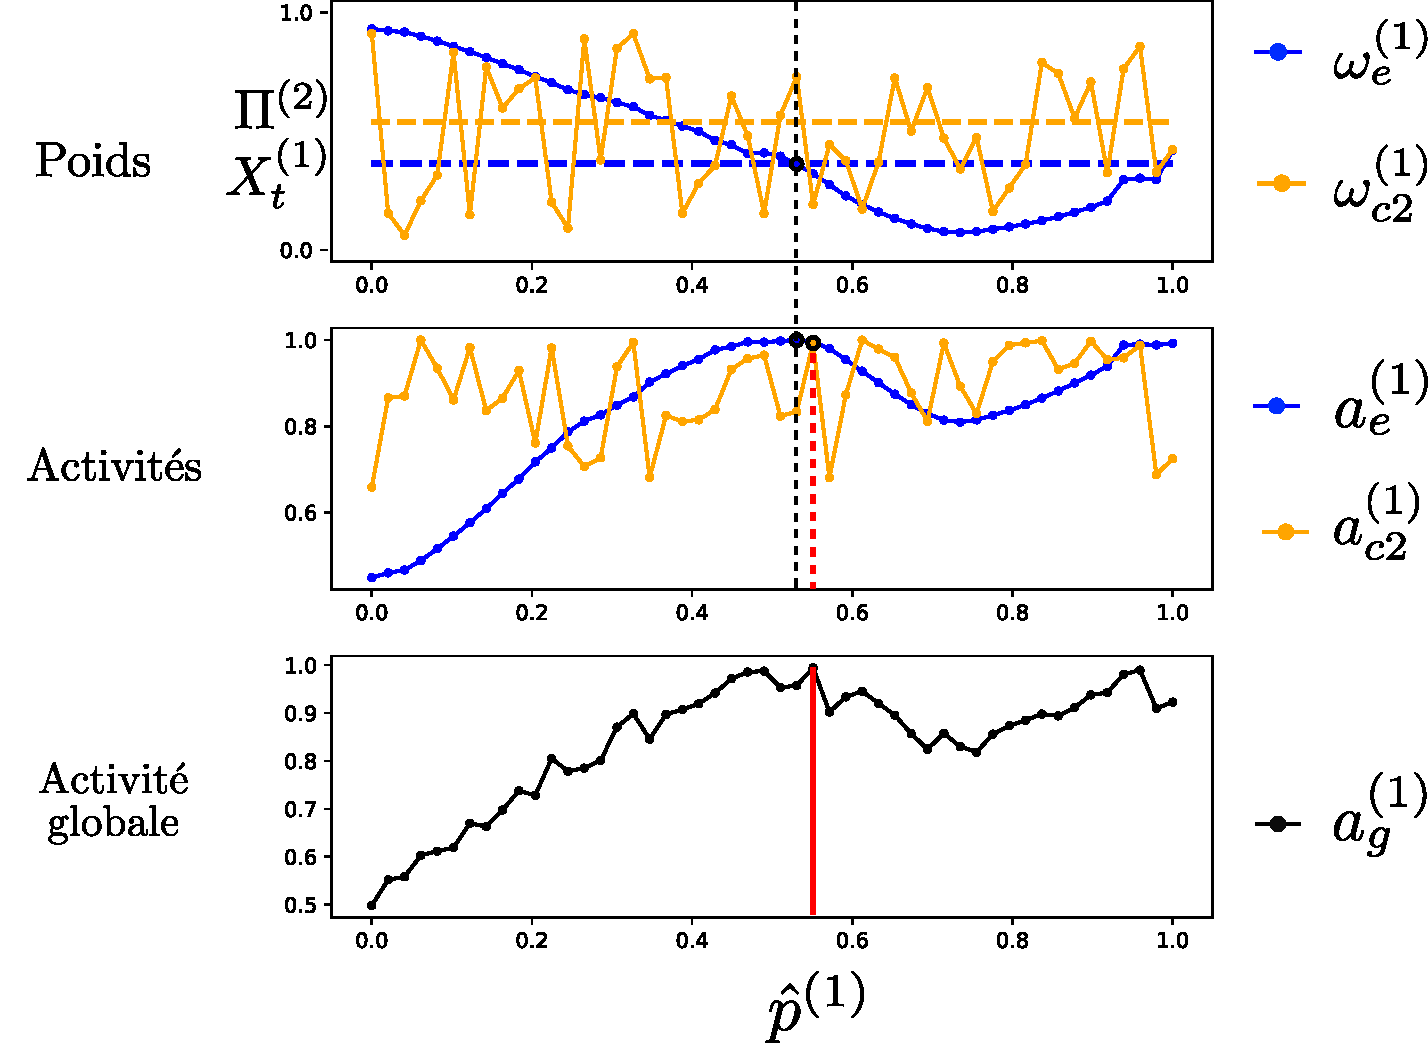
\includegraphics[width=0.8\textwidth]{activite_layers_2maps.pdf}
%\end{minipage}
%\begin{minipage}{0.35\textwidth}
\caption{Calcul d'activité dans une SOM au sein d'une architecture de deux cartes. La carte prend une entrée externe et une entrées contextuelle. L'indice $(1)$ permet de distinguer les objets relatif à cette carte. L'entrée externe est $X\m{1}_t$. La carte possède deux couches de poids, permettant de calculer deux activités. L'activité globale prend en compte tout les couches d'activités afin de trouver un BMU commun pour toutes les couches de poids. Ce calcul favorise l'activité externe et est modulé par l' activité contextuelle, ce qu'on observe sur la courbe du bas. Le maximum de l'activité globale est noté $\hat{p}$. A partir de l'activité globale, le BMU $\bmu\m{1}_t$ sera trouvé par le processus de relaxation décrit en partie~\ref{sec:relax}\label{fig:2som_activite}}
%\end{minipage}

\end{figure}

\begin{figure}
\centering
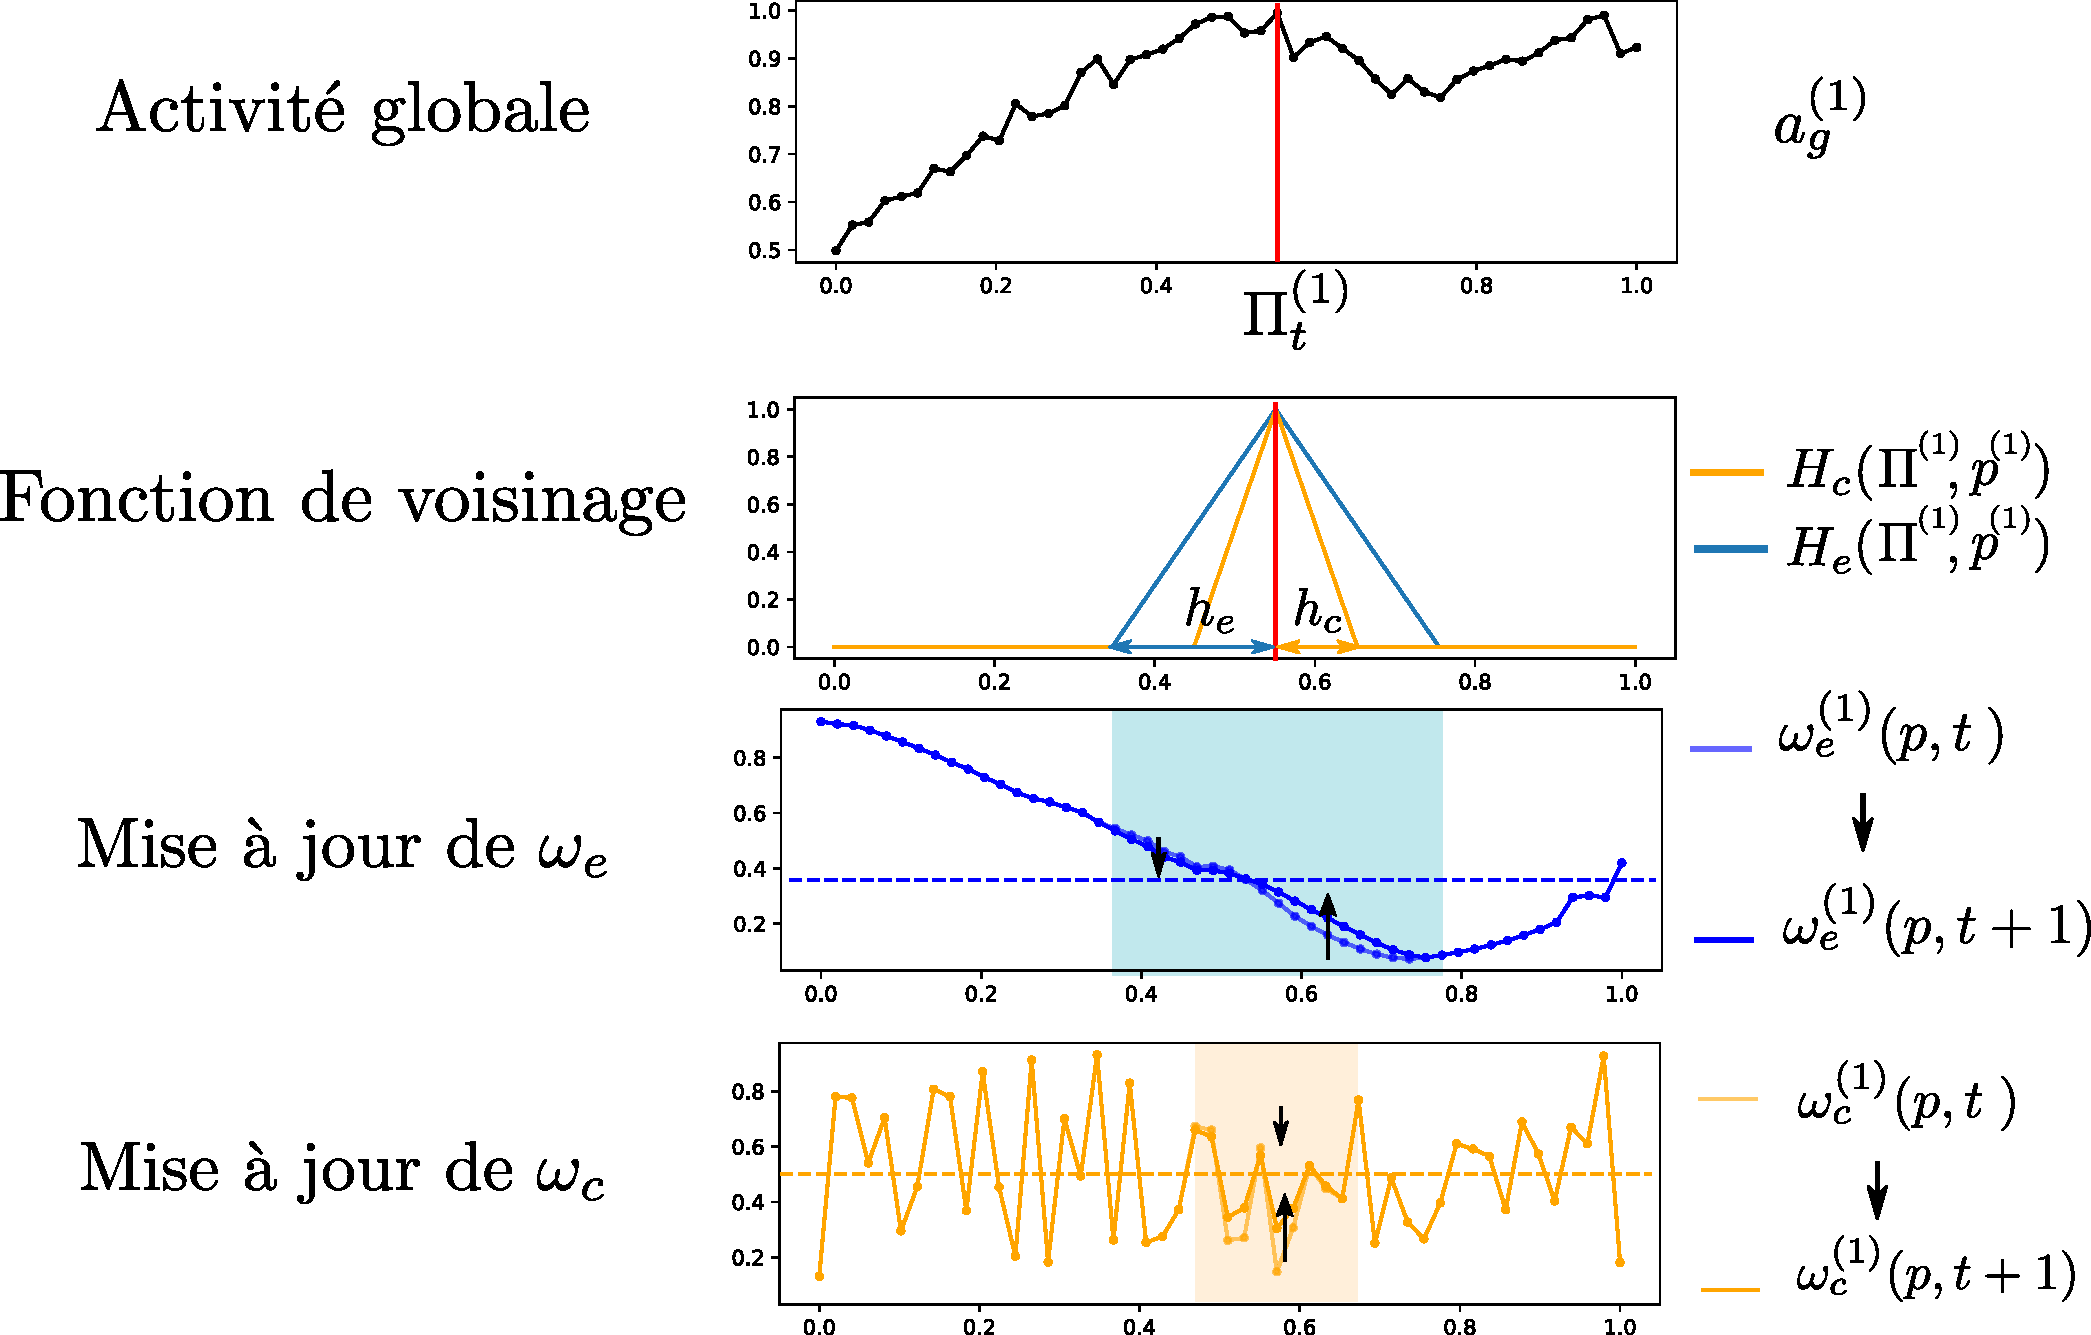
\includegraphics[width=0.9\textwidth]{maj_2som.pdf}
%\end{minipage}
%\begin{minipage}[c]{0.35\textwidth}
\caption{Mise à jour de chaque couche de poids indépendamment, relativement au BMU commun $\bmu\m{1}_t$, calculé par relaxation. Par définition de la relaxation, la position $\bmu\m{1}_t$ est proche de la position $\hat{p}\m{1}$ à la fin de la relaxation. Le rayon de voisinage $h_e$ est utilisé pour mettre à jour les poids externes, le rayon $h_c$ pour mettre à jour les poids contextuels. On choisit $h_e > h_c$. Cette différence permet une différence d'échelle d'apprentissage entre couches de poids. Elle est détaillée en section suivante.\label{fig:maj}}
%\end{minipage}
\end{figure}

\subsection{Résumé}
Les étapes d'un pas d'apprentissage $t$ d'une architecture de deux cartes sont les suivantes; elles sont schématisées en figure~\ref{fig:algo}.
\begin{enumerate}
\item Présentation des entrées $\inpx\m{1}_t$ et $\inpx\m{2}_t$ à chaque carte
\item Relaxation:
\begin{enumerate}
\item Calcul de l'activité externe $a_e(\inpx\m{i},p)$ dans chaque carte et initialisation des BMUs $(\bmu\m{1}_0,\bmu\m{2}_0)$ pour la relaxation.
\item Relaxation par petits déplacements de $\bmu\m{1}_\tau,\bmu\m{2}_\tau$ dans chaque carte, avec calcul de l'activité contextuelle et globale à chaque pas $\tau$, jusqu'à stabilisation selon $\tau$ du couple de valeurs $(\bmu\m{1}_\tau,\bmu\m{2}_\tau)$
\item Choix des positions de BMU $\bmu\m{1}_t,\bmu\m{2}_t$ comme la valeur de $(\bmu\m{1}_\tau,\bmu\m{2}_\tau)$ à l'issue de la relaxation
\end{enumerate}
\item Mise à jour des poids $\w\ext\m{i}$ et $\w\cont\m{i}$ dans chaque carte, selon la position du BMU $\bmu\m{i}$, les entrées externes $\inpx\m{i}_t$ et contextuelles $\bmu\m{j}_t$, la position du BMU calculée par relaxation dans l'autre carte.
\end{enumerate}
\begin{figure}
\centering
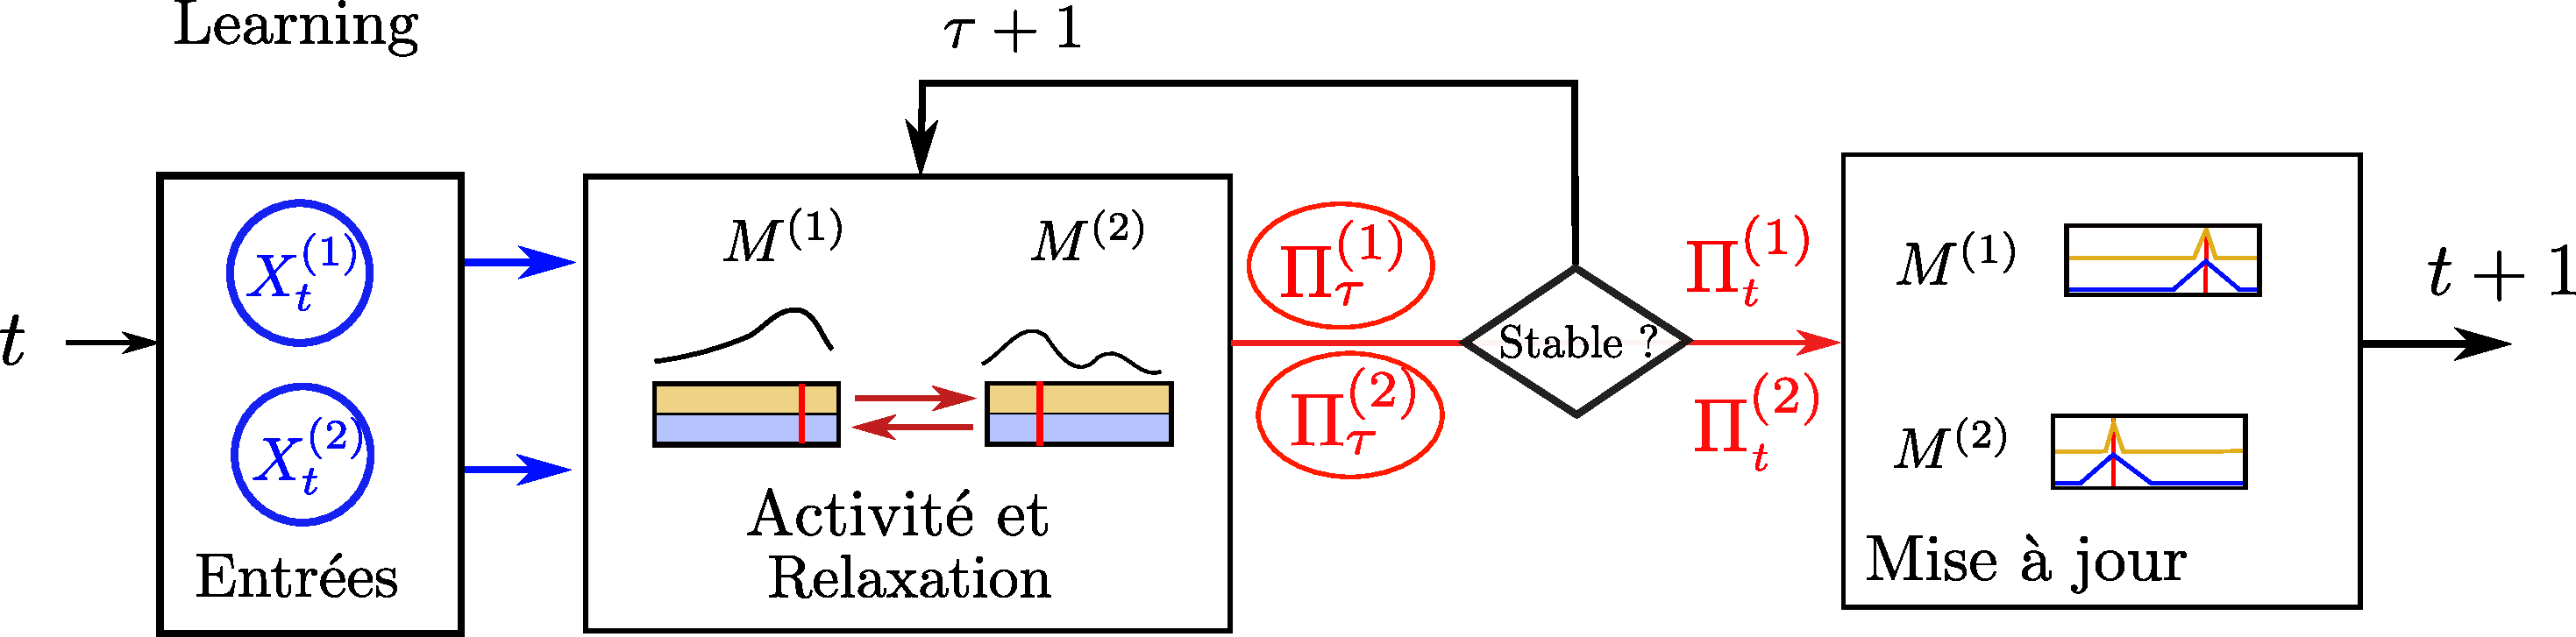
\includegraphics[width=\textwidth]{learning_tests_2maps}
\caption{Résumé des étapes de l'algorithme d'apprentissage d'une architecture.}
\label{fig:algo}
\end{figure}


\section{Formalisation: cas pour $n$ cartes}\label{sec:formalisme}

Nous présentons dans cette partie un formalisme pour l'algorithme général pour une architecture quelconque de $n$ cartes. Les notations sont valables pour des cartes de dimension quelconque; les entrées peuvent être de dimension quelconque.
La différence principale avec l'exemple à deux cartes est qu'une carte peut prendre plusieurs entrées contextuelles, qui sont les BMUs de toutes les cartes qui lui sont connectées dans l'architecture, au lieu d'une dans le cas de deux cartes. On retrouvera donc les notations de la partie précédente.
Cette partie concentre toutes les notations et l'algorithme utilisé dans cette thèse. L'algorithme est résumé en algorithme~\ref{algo:cxsom}.

\subsection{Entrées et calcul d'activité}

Nous présentons d'abord la structure et les notations utilisées dans une carte; toutes ces notations sont retrouvables en figure~\ref{fig:2som_activite}, pour l'exemple d'architecture de 2 cartes. Dans une architecture composée de $n$ cartes, les cartes sont indexées par $i \in \{1,\cdots,n\}$. On indicera chaque élément d'une carte $M\m{i}$ par l'exposant $(i)$.
Pour faciliter la lecture, nous omettrons par abus de langage l'exposant $(i)$ dans les équations, lorsqu'on se concentre sur une seule carte. $\inpx_t$ désigne donc $\inpx_t\m{i}$, $\w_e$ désigne $\w_e\m{i}$, etc.


A un pas d'apprentissage $t$, une carte $M\m{i}$ reçoit en entrée une entrée \emph{externe} notée $\inpx_t$ et $K$ entrées \emph{contextuelles}. Notons-les pour le moment $\Gamma = (\inpc_{i_1},\cdots,\inpc_{i_K})$; elles seront les positions de BMU $\bmu\m{i_k}$ des cartes d'indice $i_k$ qui lui sont connectées. La gestion des entrées contextuelles sera décrite avec le processus de relaxation en section suivante; notons pour le moment que les entrées contextuelles sont des positions 1D ou 2D dans des cartes. 

La carte possède donc $K+1$ couches de poids. On  note $\w_e(p)$ les poids externes et $\w_{ci_1}(p), \cdots, \w_{ci_K}(p)$ les poids correspondant aux entrées contextuelles, les \emph{poids contextuels}.
$\w_{ci_k}$ correspond à la couche de poids relative à l'entrée contextuelle $\inpc_{i_k} = \bmu\m{i_k}$. Les poids externes sont à valeur dans $\mathcal{D}\m{i}$, la modalité associée à la carte $i$. Les poids contextuels sont à valeur dans l'espace des positions d'une cartes, soit $[0,1]$ en 1D ou $[0,1]^2$ en 2D.

Les activités externes et contextuelles s'expriment de la façon suivante:
\begin{equation}
\label{eq:activite}
\begin{cases}
a_e(\inpx_t,p) = \exp\frac{-\lVert \w_e(p)-\inpx_t \rVert^2}{2\sigma^2} \\
a_{ci_k}(\inpc_{i_k},p) = \exp\frac{-\lVert \w_{ci_k}(p)-\inpc_{i_k} \rVert ^2}{2\sigma^2}, \\
i_1, \cdots, i_K\: \text{indices des cartes connectées à $i$ dans l'architecture}
\end{cases}
\end{equation}
Notons $a_c(\Gamma,p)$ la moyenne des activités contextuelles, avec $\Gamma = (\inpc_{i_1}, \cdots, \inpc_{i_K})$.
\begin{equation}\label{eq:ac}
a_c(\Gamma,p) = \frac{1}{K}\sum_{k=1}^K {a_{ci_k}(\inpc_{i_k},p)}
\end{equation}
L'activité globale $a_g$ est calculée en combinant l'activité externe et la moyenne des activités contextuelles:
\begin{equation}
\label{eq:global_act}
a_g(\inpx_t,\Gamma,p) = \sqrt{a_e(\inpx_t,p) \frac{a_e(\inpx_t,p) +  a_c(\Gamma,p)}{2}}
\end{equation} 
On note $\hat{p}$ la position du maximum de l'activité globale:
\begin{equation}
\label{argmax}
\hat{p} = \argmax_p a_g(\inpx_t, \Gamma,p)
\end{equation}

Notons qu'une carte peut ne pas avoir d'entrée externe: toutes ses entrées sont des positions des BMUs d'autre cartes. Dans ce cas, on prendra comme activité globale $a_c$, la moyenne des activités contextuelles (équation~\ref{eq:ac}).

\subsection{Calcul du BMU par relaxation}\label{sec:relax}

Dans chaque carte $i$, l'entrée contextuelle $\inpc\m{i}_{i_k}$ est le BMU $\bmu\m{i_k}$  de la carte $i_k$. Le BMU $\bmu\m{i}$ dépend donc de ceux des autres cartes, qui dépendent eux-mêmes de $\bmu\m{i}$. Au lieu de chercher un maximum d'activité indépendamment dans chaque carte, on doit donc résoudre un problème d'optimisation global à  l'architecture. On cherche les positions $\mathbf{\bmu} = (\bmu\m{1}, \cdots, \bmu\m{n})$, si elles existent, telles que:
\begin{equation}
\forall i, \; \bmu\m{i} = \argmax_{p\m{i}} a_g\m{i}(\inpx\m{i}_t, \bmu\m{i_1}, \cdots, \bmu\m{i_K},p\m{i})
\end{equation}
$\bmu\m{i_1}, \cdots, \bmu\m{i_K}$ est un sous ensemble de $\mathbf{\bmu}$. On peut donc écrire $\bmu\m{i} = \argmax_{p\m{i}} a_g\m{i}(\inpx\m{i}_t, \mathbf{\bmu}, p\m{i})$
Si cette position n'existe pas, on cherche le meilleur compromis, c'est à dire les positions $\bmu\m{i}$ telles que l'activité globale de chaque carte soit la plus élevée possible.
%TODO ???
Pour formuler le problème en terme d'optimisation, on cherche le vecteur $\mathbf{\bmu} = (\bmu\m{i})_{i=1 \cdots n}$ minimisant, pour tout $i$, $\lVert \bmu\m{i} - \argmax_{p\m{i}} a_g\m{i}(\inpx\m{i}_t, \mathbf{\bmu}, p\m{i}) \rVert$


Le processus de relaxation est une boucle imbriquée dans un pas d'apprentissage de l'architecture, indexée par $\tau$. Notons $\bmu\m{i}$ la position du BMU de la carte $i$, et $\mathbf{\bmu} = (\bmu\m{0}, \cdots , \bmu\m{n})$, avec $n$ le nombre de cartes de l'architecture.

On cherche, dans chaque carte $i$, la position $\bmu\m{i}$ telle que $\forall i, a_g\m{i}(\bmu\m{i},\inpx\m{i},\bmu\m{i_0},\cdots,\bmu\m{i_k})$ soit maximale.
Au début d'un pas d'apprentissage, chaque carte est nourrie avec une entrée externe $\inpx\m{i}_t$ qui restera constante au cours de la relaxation. Les activités externes $a_e\m{i}(\inpx\m{i}_t,p)$ de chaque carte peuvent être calculées.
La recherche du BMU suit le processus de relaxation suivant :
\begin{enumerate}
\item Dans chaque carte $i$, la position $\bmu\m{i}$ est initialisée à $\hat{p}\m{i}_0 = \argmax_{p\m{i}}(a_e\m{i}(\inpx\m{i}_t,p)$. Dans chaque carte $i$, on assigne $\inpc_{i_k}\m{i} = \bmu\m{i_k}_\tau$
\item Tant que toutes les positions $\bmu\m{i}$ ne sont pas stables, 
	\begin{enumerate}
	\item Dans chaque carte $i$, calculer les activités contextuelles et globales, définissant ainsi $\hat{p}\m{i}_\tau = \argmax_{p\m{i}}(a_g\m{i}(p\m{i},\inpx\m{i}, \bmu\m{i_0}_\tau,\cdots,\bmu\m{i_k}_\tau)$, avec $i_0, \cdots, i_k$ les indices des cartes connectées à $i$ dans l'architecture.
	\item Déplacer $\bmu\m{i}$ vers $\hat{p}\m{i}$ : $\bmu\m{i}_{\tau +1} \leftarrow \bmu\m{i}_\tau + \Delta \times \sign(\hat{p}\m{i} - \bmu\m{i})$ si $\lvert \bmu\m{i}- \hat{p}\m{i}\rvert \geq \Delta$, $\bmu\m{i} \leftarrow \hat{p}\m{i}$ sinon
	\end{enumerate}
\item Le BMU de chaque carte est pris comme la valeur finale stable de ce processus dynamique. Cette valeur est utilisée pour les mises à jour des poids.
\end{enumerate}

Il peut arriver que les positions ne trouvent pas de point de stabilité. Dans ce cas, on arrêtera la relaxation arbitrairement; ce phénomène étant ponctuel, il n'influence pas l'apprentissage. Les paramètres des cartes de l'architecture sont choisis pour éviter de telles situations.
Nous étudierons plus en détail ce processus de relaxation.

\subsection{Mise à jour des poids}
Les poids sont mis à jour par rapport à leurs entrées respectives suivant l'équation \ref{eq:update}. Le BMU d'une carte est ainsi commun à toutes les couches. 
Les rayons de voisinage $h_e$ et $h_c$ ont des valeurs différentes.
Ainsi, on peut vraiment voir la mise à jour des poids d'une carte comme indépendante à chaque couche, avec des paramètres propres, ayant simplement le BMU en commun.
\begin{align}
 \w\ext\m{i}(p,t+1) = \w\ext\m{i}(p,t) + H\ext(\bmu\m{i}, p)(\w\ext\m{i}(p) - \inpx_t\m{i}) \\
\forall k, \w_{ci_k}\m{i}(p,t+1) = \w_{ci_k}\m{i}(p) + H\cont(\bmu\m{i},p)(\w_{ci_k}\m{i}(p) - \bmu\m{i_k}_t)
\end{align}


\begin{algorithm}\label{algo:cxsom}
\caption{Déroulement d'une itération d'apprentissage $t$}
\SetAlgoLined
  \KwData{$\inpx\m{1}_t, ... , \inpx\m{K}_t$ tirés dans $\mathcal{D}\m{1} \times \cdots \times \mathcal{D}\m{n}$}
  $\tau \leftarrow 0$\\
  \lForEach{carte $i$}{$\bmu\m{i}_0 \leftarrow \argmax_{p\m{i}} a\ext(\inpx\m{i}_t,p\m{i})$}
  \While {$\mathbf{\bmu}_\tau \neq \mathbf{ \bmu}_{\tau-1}$ et $\tau < \tau_{max}$}{
  \ForEach{carte $i$}{
 	Avec $i_1, \cdots i_K$ indices des cartes connectées à $i$ dans l'architecture:
	Calcul de $a_{ci_1}\m{i}(\bmu\m{i_1},p\m{i}), \cdots, a_{ci_k}\m{i}(\bmu\m{i_K},p\m{i})$\\
  	Calcul de $a_g\m{i}(\inpx\m{i}, \bmu\m{i_0}_\tau, \cdots, \bmu\m{i_k}_\tau)$ (equation~\ref{eq:global_act})\\ 
  $\hat{p}\m{i}_\tau = \argmax_{p\m{i}} a_g\m{i}(\inpx\m{i}, \bmu\m{i_1}_\tau, \cdots, \bmu\m{i_K}_\tau)$ \\
  Déplacement de $\bmu\m{i}_\tau$ vers $\hat{p}\m{i}$ d'un pas $\Delta$:
  $\bmu\m{i}_{\tau+1} \leftarrow \bmu\m{i}_\tau + min(\Delta, \lvert \hat{p}\m{i} - \bmu\m{i}_\tau \rvert) \times \sign(\hat{p}\m{i} - \bmu\m{i}_\tau)$
  }
  $\tau \leftarrow \tau + 1$
  }
  $\bmu\m{1}_t, \cdots, \bmu\m{n}_t \leftarrow \hat{p}\m{1}_\tau, \cdots , \hat{p}\m{n}_\tau$\\
  \ForEach{Carte $i$}{
  $\w\ext\m{i}(p) \leftarrow \w\ext\m{i}(p) + H\ext(\bmu\m{i}_t, p)(\w\ext\m{i}(p) - \inpx_t\m{i})$\\
  \lForEach{$k$}{$\w_{ci_k}\m{i}(p) \leftarrow \w_{ci_k}\m{i}(p) + H\cont(\bmu\m{i}_t,p)(\w_{ci_k}\m{i}(p) - \bmu\m{i_k}_t)$}
  }
 \end{algorithm}
 



\draft{
\subsection{Etape de test}

Afin d'étudier le dépliement des cartes, on effectue des itérations de \emph{test} pendant l'apprentissage. Ces étapes consistent à effectuer les étapes de présentation d'entrée, calcul d'activité et recherche du BMU par relaxation, mais pas l'étape de mise à jour des poids. Les poids des cartes restent donc figés pendant un ensemble de tests. Les entrées des cartes sont $\inpx\m{i}_t$, issues d'un ensemble de test, du même espace que les entrées servant à l'apprentissage.
}

\draft{
\subsection{Prédiction d'entrée}
Par construction, une carte de l'architecture CxSOM peut ne pas avoir d'entrée externe. Les activités considérées pour la recherche du BMU seront alors les activités contextuelles. On peut ainsi utiliser CxSOM pour des tâches de prédiction. Les données présentée à l'architecture sont $\inpx\m{1}, \cdots, \inpx\m{n}$, $n$ modalités. Ces modalités portent de l'information les unes sur les autres. 
L'architecture de cartes peut être vue comme un système dynamique réagissant à des données d'entrées.
}
\section{Choix des paramètres}\label{sec:params}

Le modèle CxSOM introduit des paramètres supplémentaires par rapport à une carte classiques. Les plages de valeur utilisées pour tous les paramètres d'une architecture sont résumées en tableau~\ref{tab:params}
\subsection{Paramètrage d'une carte}
On retrouve les mêmes paramètres dans CxSOM que sur une carte classique: taille de la carte, topologie et dimensions. 
Contrairement à une carte simple, on a maintenant un jeu de paramètre d'apprentissage par couche de poids d'une carte : pour chaque couche de poids $\w_e$ et $\w_{ci_k}$, on peut faire varier le taux d'apprentissage $\alpha$ et le rayon de voisinage $h_e$ ou $h_{ci_k}$. Le taux d'apprentissage $\alpha$ est commun à toutes les couches dans un souci de simplicité.

On choisit de prendre une valeur $h_{ci_k} = h_c$ commune à toutes les couches de poids contextuels d'une carte. Ainsi, on apporte une symétrie dans les connexions: les carte réagissent de la même façon aux autres cartes. Le rayon externe, par contre, est choisi $h_e$ très supérieur au rayon contextuel. Nous prendrons au moins $h_e = 10 h_c$. Cette différentiation de paramètres apporte deux élasticités dans l'apprentissage, et induit deux vitesses de dépliement dans la carte sans avoir à modifier les paramètres au cours de l'apprentissage. Les poids externes se déplient alors très rapidement sur les données, quand les poids contextuels se déplacent très peu au début. Lorsque les poids externes sont organisés, l'apprentissage n'influence plus que les poids contextuels et ces derniers se déplient. Nous analyserons plus en détail l'organisation des cartes dans le chapitre suivant.
$\alpha$ et $h_e, h_c$ resteront constants au cours de l'apprentissage.
Ce jeu de paramètres est ajustable indépendamment dans chaque carte de l'architecture; dans nos travaux, on prendra en général les mêmes valeurs pour toutes les cartes d'une architecture.

\subsection{Paramètres de l'architecture}
Certains paramètres sont relatifs à l'architecture. Il s'agit d'abord de $\Delta$, le pas d'apprentissage. Nous avons pris la même valeur de pas pour toutes les cartes. Cette valeur sera en général d'ordre $0.1$, c'est à dire un déplacement de $10\%$ de la taille de la carte, dans les expériences présentées dans les chapitres suivants. Nous verrons que la valeur de ce paramètre a finalement peu d'influence sur la relaxation; il faut juste veiller à ne pas le prendre trop petit, pour ne pas augmenter les temps de relaxation. Le deuxième paramètre relatif à la relaxation est $\tau_{max}$, nombre maximum de pas de relaxation. Il sera fixé à 200 dans la plupart de nos expériences; nous verrons que la relaxation, si elle converge, se réalise en une dizaine de pas.
Les connexions entre cartes sont prédéfinies et fixes. On choisit donc au préalable la taille de l'architecture et les connexions entre cartes.

\begin{table}
\caption{Tableau récapitulatif des paramètres ayant une influence sur le comportement de l'algorithme CxSOM. Tous les paramètres relatif à une carte sont les mêmes pour chacune des cartes de l'architecture, mais il est possible de les différencier. L'analyse de l'influence des paramètres sera détaillée au chapitre~\ref{chap:analyse}.}\label{tab:params}
\vspace{3mm}
\begin{tabular}{|c|c|c|}
\hline
Paramètres & Description & Plage de valeur \\
\hline
$\alpha$ & Taux d'apprentissage & $0.1$ \\
$N$ & Taille de la carte & de $500$ à $1000$ en 1D, $50 \times 50$ en 2D \\
$\h_e$ & Rayon de voisinage externe & autour de $0.2$ \\
$h_c$ & Rayon de voisinage contextuel & D'ordre $\frac{h_e}{10}$ ou inférieur) \\
$\Delta$ & Pas de relaxation & $0.1$ \\
$\tau_{max}$ & Nombre de pas de relaxation maximum & 200 \\
\hline
\end{tabular}
\end{table}


\section{Conclusion}

le modèle CxSOM permet de construire une architectures de carte auto-organisatrices apprennant chacune sur des entrées de différent types, mais liées par un modèle: des entrées multimodales. L'apprentissage est couplé entre cartes par l'utilisation d'entrée contextuelles dans chaque carte, qui sont les positions des BMU qui lui sont connectées. Nous avons décrit dans ce chapitre l'algorithme permettant d'effectuer l'apprentissages de données dans une telle architecture ainsi que les notations associées.

L'algorithme d'apprentissage a été conçu de façon large: nous avons développé un modèle général permettant d'associer des cartes. Les objectifs des chapitres suivants sont d'abord de montrer le comportement de l'algorithme et comment la relaxation permet de déterminer un BMU dans chaque carte. Nous étudierons ensuite en détail comment les données fournies en entrées à une architecture sont représentées dans les couches de poids. Nous verrons enfin une application d'une architecture de cartes dans un contexte de prédiction d'entrée.

\draft{
\Annexes
\Annex{Glossaire des notations}
\begin{itemize}
\item $\inpx_t$ Entrée externe présentée à la carte à l'itération d'apprentissage $t$. $\inpx_t \in \mathcal{D}$
\item $\inpc$ Entrée contextuelle d'une carte. Les entrées contextuelles sont les positions des BMUs $\bmu\m{i_k}$ d'autres cartes de l'architecture; on notera $\inpc_{i_k}$ l'entrée contextuelle liée à la carte $i_k$.
\item $p$ indexation des n\oe{}uds carte, $p \in [0,1]$ ou $[0,1]^2$.
\item $\w\ext(p)$ Poids externes. $\w\ext \in \mathcal{D}$
\item $\w_{ck}(p)$ Couche de poids contextuels d'une carte liés à l'entrée $\inpc_{i_k}$. $\w_{ck}(p) \in [0,1]$ ou $[0,1]^2$.
\item $a_e(\inpx_t,p)$ Activité externe 
\item $a_{ck}(\inpc_{i_k},p)$ Activité contextuelle calculée sur la couche de poids $w_{ck}$
\item $a_c(\Gamma,p)$ Moyenne des couches activités contextuelles
\item $a_g(\inpx_t,\Gamma,p)$ Activité globale, combinaison des activités externes et contextuelles
\item $\bmu_\tau$ Positions intermédiaires des BMUs d'une carte pendant la relaxation
\item $\bmu_t$ Position finale du BMU d'une carte après relaxation
\end{itemize}
}

\chapter{Méthodes de représentation et d'analyse de l'architecture CxSOM}
\graphicspath{{03-Representation/}}

\minitoc
\section{Représentation des cartes de Kohonen}

\subsection{Représentations et indicateurs classique des cartes de Kohonen}

Les cartes de Kohonen sont particulièrement associées à une facilité de représentation et de visualisation. En effet, leur nombre réduit de prototypes et leur aspect topologique permet d'en tracer une représentation visuelle interprétable.
La manière la plus utilisée de représenter une carte de Kohonen est de tracer les poids de ses prototypes, disposés dans le graphe qu'est la carte. En fonction des dimensions des entrées, cette représentation prennent plusieurs formes. Deux exemples courants de représentation sont les suivants: 
\begin{itemize}
\item Le graphe qu'est la carte de Kohonen est représenté dans l'espace de ses positions (la grille d'indices $(i,j)$, ou une ligne indexée par $i$. Sur chaque noeud est tracé le poids correspondant. C'est le cas sur l'exemple de gauche en figure~\ref{fig:representation} dans lequel les poids des prototypes, qui sont des imagettes, sont affichés en chaque point de la grille. Si la dimension d'un poids est trop grande pour être représentée graphiquement, il est également courant d'étiquetter chaque prototype et d'afficher ces étiquettes sur les noeuds de la carte, en tant que représentation.
\item Lorsque les données traitées sont des points deux ou trois dimensions, les poids des prototypes peuvent être directement tracés dans l'espace $\mathbb{R}^2$ ou $\mathbb{R}^3$. Ces poids sont alors reliés en fonction des positions des noeuds dans la carte, montrant ainsi la déformation de la carte dans l'espace d'entrée, c'est le cas sur l'exemple de droite en figure~\ref{fig:representation}.
\end{itemize}

\begin{figure}
\begin{minipage}{0.5\textwidth}
\centering
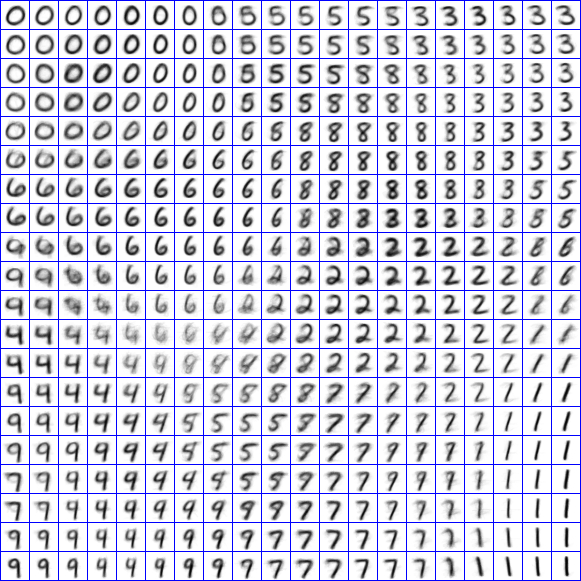
\includegraphics[width=0.5\textwidth]{digits.jpg}
\end{minipage}
\begin{minipage}{0.5\textwidth}
\centering
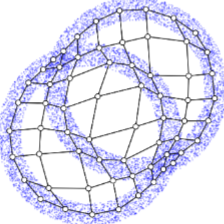
\includegraphics[width=0.5\textwidth]{points.png}
\end{minipage}
\label{fig:representation}
\caption{Représentations possible des poids d'une carte de Kohonen classiques, dans le cas d'entrées sous forme d'imagettes ou de points en deux dimensions.}
\end{figure}

\draft{Distortion d'une carte : une mesure de la différence moyenne des entrées par rapport à tous les centroïdes}

%
%On parle ici d'interprétation visuelle humaine. Pour l'oeil humain, cette facilité d'interprétation est limitée à un domaine d'utilisation: celui dans lequel les éléments qui nous intéressent sont les distances euclidiennes entre les données, ou plus généralement dans lequel la distance considérée pour la mise a jour des cartes possède un aspect graphique facilement interprétable. Essayez par exemple de vous représenter des distances dans un espace non-euclidien, ou des distances . Savoir quels points sont les plus proches nécessite alors un effort mental important et non une seule intuition; finalement la façon la plus simple de le savoir est de faire le calcul.
 
%La représentation d'une carte cherche à répondre à la question: "est-ce que la carte est bien dépliée sur toutes les données ? Est-ce qu'un prototype représente correctement une donnée ?". Y répondre en visualisant ses prototypes revient au processus intellectuel suivant: l'observateur imagine une donnée, par exemple une imagette d'un chiffre à main levée, et reproduit le processus de sélection du BMU qui a eu lieu lors de l'apprentissage de la carte pour trouver le poids qui lui correspond le mieux. Via ce processus mental, on est capable d'évaluer si une carte est dépliée sur les données. 
%Imaginons à présent que les distances considérées entre les éléments d'une carte ne soient plus euclidiennes: cette évaluation du dépliement de la carte repose maintenant sur soit une capacité d'abstraction phénoménale de l'observateur. Un exemple est donné en figure~\ref{fig:non_eucl}: l'observateur humain visualise un distance euclidienne($L^2$), éventuellement une distance de Manhattan. Mais si les distance sont calculées autrement, l'observateur préferera les nombres à la représentaiton graphique, ou une représentation dans un espace qui lui est familier. La représentation de la carte doit ainsi être adaptée au processus d'organisation.
%% Ajouter ref : mesures usuelles des cartes de Kohonen ? Pourquoi ne les utilise ton pas ?
%
% 
%Ainsi, pour représenter un algorithme d'apprentissage non-supervisé et en particulier une carte de Kohonen, on doit d'abord bien poser ce qu'on cherche à évaluer : l'entrée de l'algorithme est bien définie, sa sortie correspond à tous les éléments présents dans la carte. Un choix de représentation est donc à réaliser. Ensuite, cette représentation doit être adaptée aux règles de calcul de l'algorithme, ici de l'espace de la carte. 


\subsection{Que cherche t-on à représenter dans CxSOM ?}

Nous présenterons dans ce chapitre les choix de tracés et représentation des cartes auto-organisatrices utilisées dans une architecture CxSOM.
Les exemples de représentations présentés tout au long de ce chapitre s'appuient sur l'expérience illustrée en figure~\ref{fig:exp}: nous étudions une architecture composée de deux cartes en une dimension, chacune étant connectée à sa voisine. Les entrées des cartes sont $X$ et $Y$, les coordonnées d'un cercle. Ces deux modalités sont dépendantes: pour une valeur de $X$, deux valeurs sont possible pour $Y$, et symmétriquement.

\begin{figure}
\begin{minipage}{0.4\textwidth}
\centering
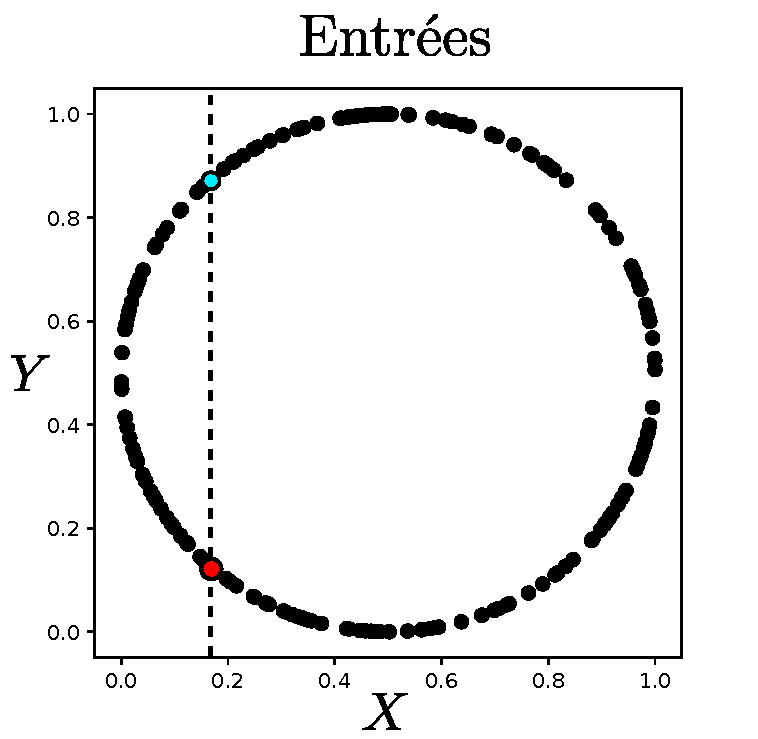
\includegraphics[width=0.8\textwidth]{2som_inp_noinformation}
\end{minipage}
\begin{minipage}{0.6\textwidth}
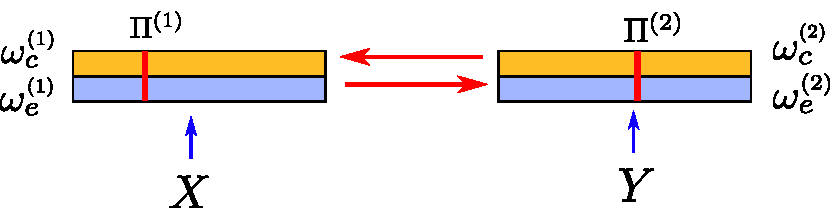
\includegraphics[width=\textwidth]{2som_archi}
\end{minipage}
\label{fig:exp}
\caption{Disposition des entrée, sous forme de cercle, à gauche, et architecture de deux cartes en une dimension étudiée et représentée dans ce chapitre.}
\end{figure}

La figure~\ref{fig:weights} présente le tracé des poids des deux cartes de l'exemple après apprentissage. Ce tracé permet de conclure que les cartes sont bien dépliées et ont transcrit une continuité dans les ensemble d'entrée. Cependant, il manque l'information nécessaire pour comprendre les mécanismes impliqués dans l'apprentissage de ces cartes. En effet, le choix du BMU dépend de plusieurs entrées et du processus de relaxation. La représentation des poids seuls ne permet pas de comprendre quels seront les BMUs de chaque carte pour une entrée donnée. 


La représentation visuelle d'une cartes d'une architecture est limitée par la dimension des entrées et la dimension des cartes. Dans l'exemple, les entrées et les cartes sont en une dimension, représenter leurs poids est donc réalisable; en plus grande dimension, il sera nécessaire d'utiliser une représentation telle que celle décrite en figure~\ref{fig:representation}. Le nombre de connexions contextuelles limitera alors également la lecture d'un tracé. Cette difficulté de représentation soulève la nécessité de définir des valeurs indicatrices du fonctionnement de la carte, calculables en grande dimension.

\begin{figure}
\centering
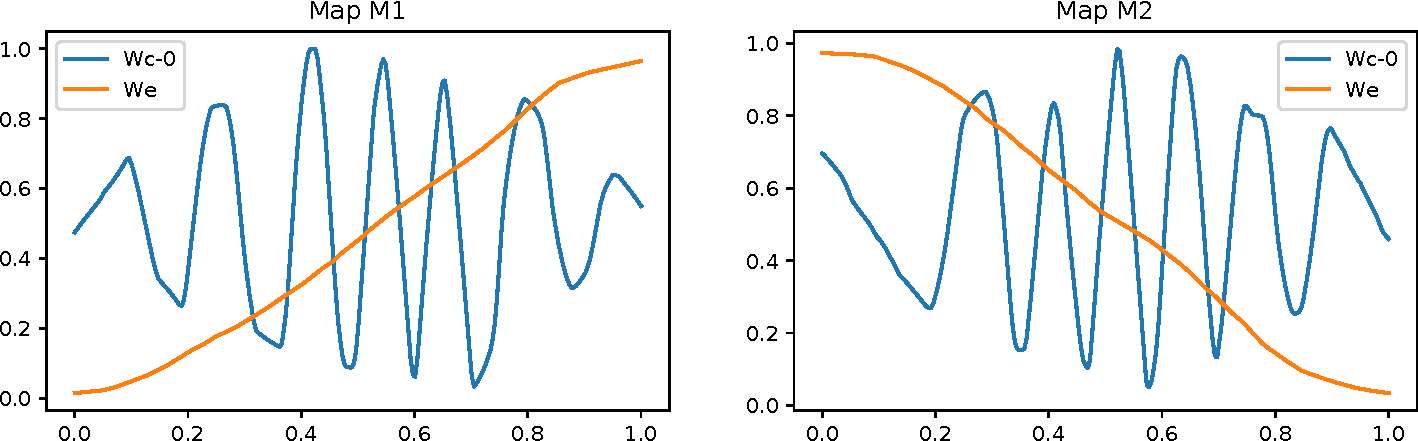
\includegraphics[width=0.9\textwidth]{weights_cercle1.pdf}
\label{fig:weights}
\caption{Représentation des valeurs des poids d'une carte au sein de CxSOM après apprentissage. La seule représentation de ces poids ne suffit pas à savoir comment la carte se comporte.}
\end{figure}

Ensuite, CxSOM s'intéresse à la communication entre cartes et la représentation des dépendances entre modalités. Représenter les cartes une à une laisse donc de coté leur connexion. Il est donc nécessaire de trouver un moyen de représenter l'architecture comme un tout. La représentation cherchera notamment à montrer comment l'architecture de cartes est capable d'apprendre les relations entre les entrées multimodales.

Ce chapitre questionne donc la façon de représenter une carte au sein d'une architecture. Nous présenterons en premier lieu un formalisme décrivant les cartes et leurs entrées multimodales associées. A partir de ce formalisme, nous proposerons plusieurs représentations et indicateurs permettant de comprendre et représenter ce que calcule une architecture CxSOM sur les données d'entrées. Nous utiliserons ces représentations et indicateurs dans les chapitres suivants. 

\section{Formalisme: variables aléatoires}

Nous introduisons dans cette section un formalisme traitant les éléments des cartes et les entrées en tant que variables aléatoires. Ce formalisme a l'avantage de à la fois clarifier les représentations, et de permettre le développement d'indicateurs statistiques sur les cartes.

\subsection{Représentation des entrées}

Les observations multimodales que l'on cherche à apprendre par l'architecture de cartes sont notées ${\inpx\m{i}, i = 0 \cdots N}$ où $N$ est le nombre de modalités considérées. A chaque pas de temps, un vecteur $\mathbf{\inpx} = (\inpx\m{0}, \cdots , \inpx\m{N})$ est présenté à l'architecture. Il s'gait d'une réalisation de la variable jointe $\mathbf{X}$.

On s'intéressera particulièrement à l'apprentissage de relations entre entrées. Les variables $\inpx\m{i}$ ne sont donc pas des variables indépendantes. On choisit  de représenter cette dépendance par une autre variable aléatoire $U$. Cette variable est multidimensionnelle et choisie de façon à ce que chaque variable $\inpx\m{i}$ soit une fonction quelconque de la variable aléatoire $U$, et uniquement de cette variable.

\begin{equation}
\forall i, \inpx\m{i} = f\m{i}(U)
\label{eq:U}
\end{equation}

Il s'agit d'une réduction de dimension qui traduit l'existence d'un modèle reliant les observations.
Dans le cas d'exemple, $\mathbf{X} = (X,Y)$, les coordonnées cartésiennes des points du cercle est alors une vecteur aléatoire, dont les composantes sont les variables aléatoires $X,Y$. En définissant une variable $U$ à valeurs réelles, chaque point du du cercle peut maintenant s'écrire, selon l'équation paramétrique du cercle:
\begin{equation}
 \begin{cases}
     X = r  \cos(2\pi U)\\
     Y = r \sin(2 \pi U)
    \end{cases}\,.
\end{equation}

$U$ représente ici l'angle du point sur le cercle. $U$ est une variable cachée qui réduit la dimension du modèle. Et contient toute l'information sur l'échantillon. 
$U$ et $f\m{i}$ ne sont pas uniques. Elle sont choisies en fonction de ce qu'on cherche à traduire dans le modèle. Ainsi, pour le même ensemble de points sous forme de cercle, on pourrait aussi définir une variable $U$ en deux dimensions, une dimension à valeur réelles paramétrisant un demi cercle, l'autre à valeurs dans ${0,1}$ indiquant de quel coté de l'axe des abscisses on se situe. Ces paramétrisations sont exprimées en figure \ref{fig:U}.
Par contre, la plus petite dimension possible de $U$ dépend du degré de liberté du modèle. Si toutes les observations se situent sur une courbe de dimension 1, alors il existe une variable $U$ en une dimension satisfaisant l'équation~\ref{eq:U}. Si les observations se situent sur une surface de dimension 2, alors, $U$ sera en deux dimensions, et ainsi de suite. 
Les exemples donnés sont scalaires, mais cette représentation générale à n'importe quel dimension et nombre d'entrées.

\begin{figure}
\begin{minipage}{0.5\textwidth}
\centering
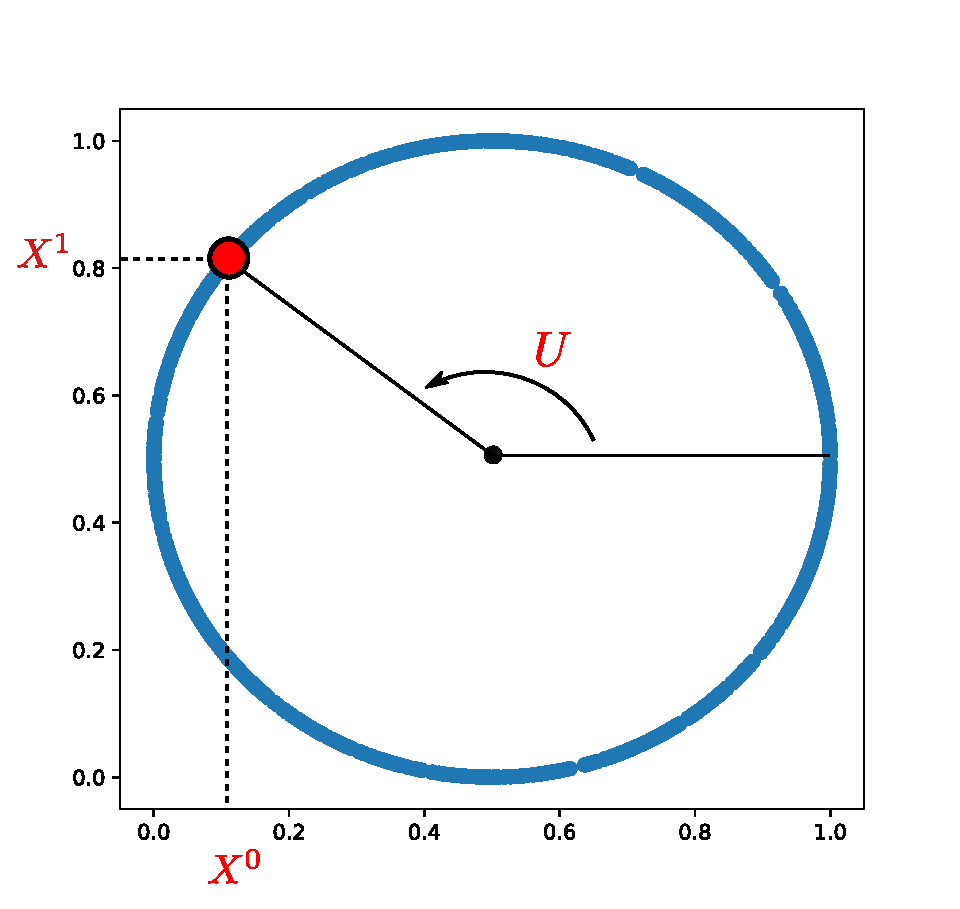
\includegraphics[width=0.6\textwidth]{cercle.pdf}
\end{minipage}
\begin{minipage}{0.5\textwidth}
\centering
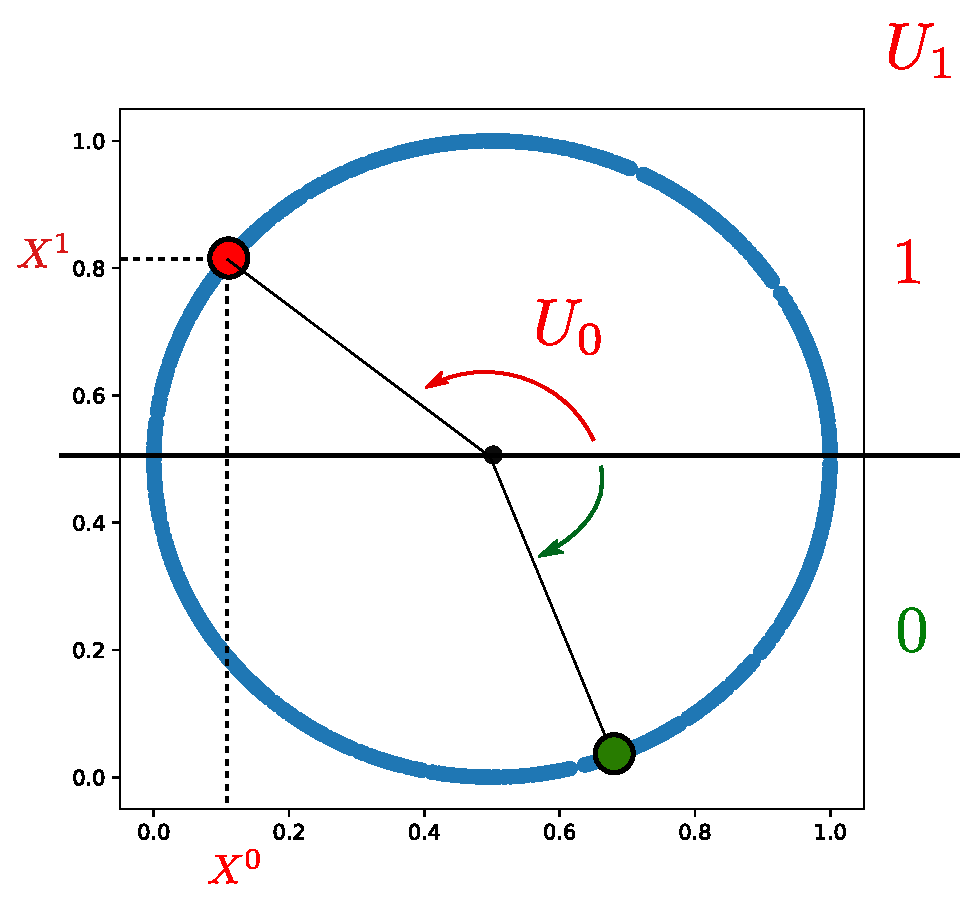
\includegraphics[width=0.6\textwidth]{cercle_2.pdf}
\end{minipage}
\label{fig:U}
\caption{Exemples de paramétrisations du cercle. La paramétrisation qui traduit le plus facilement le modèle est naturellement celle dans laquelle $U$ est à valeurs réelles. Le modèle auxquelles appartiennent les modalités $X^0$ et $X^1$ est donc représenté par la variable cachée $U$.}
\end{figure}

\subsection{Représentation des éléments des cartes}

Le jeu de données d'entrée se décompose en jeu d'apprentissage et jeu de tests. Lors de la phase de test, seul le processus de recherche de la best matching unit est réalisé et les poids des cartes ne sont pas mis à jour. Dans le cadre des variables aléatoires, chaque itération de test est alors un tirage indépendant. Les éléments des cartes peuvent donc être considérés comme des variables aléatoire et une itération de test comme une réalisation de celles-ci. La phase de test peut être réalisée après n'importe quelle itération de l'algorithme d'apprentissage. Le processus d'apprentissage et de tests est décrit en figure~\ref{fig:flowchart}.

Nous considérerons alors plusieurs éléments des cartes en tant que variables aléatoires:  
\begin{itemize}
\item Les positions des BMUs $\bmu\m{0}, \cdots, \bmu\m{N}$ dans chaque carte
\item Les poids externes des BMUs $\w_e\m{0}(\bmu\m{0}), \cdots, \w_e\m{N}(\bmu\m{N})$
\end{itemize}
Tout autre élément d'une carte peut être vu de cette manière, telles que les activités. 
Une phase de test est alors un ensemble de réalisations d'une variable aléatoire jointe : 
$$(\inpx\m{0}, \cdots, \inpx\m{N}, \bmu\m{0}, \cdots, \bmu\m{N}, \w_e\m{0}(\bmu\m{0}), \cdots, \w_e\m{N}(\bmu\m{N}))$$
Les composantes de cette variable jointe ne sont pas indépendantes. Les représentations et indicateurs présentés ensuite chercheront à détecter et comprendre au mieux leurs dépendances statistiques.

Le formalisme par variable aléatoires permet alors d'utiliser des outils et métriques issus de la théorie de l'information pour qualifier l'organisation des cartes au sein de l'architecture.

\begin{figure}
\centering
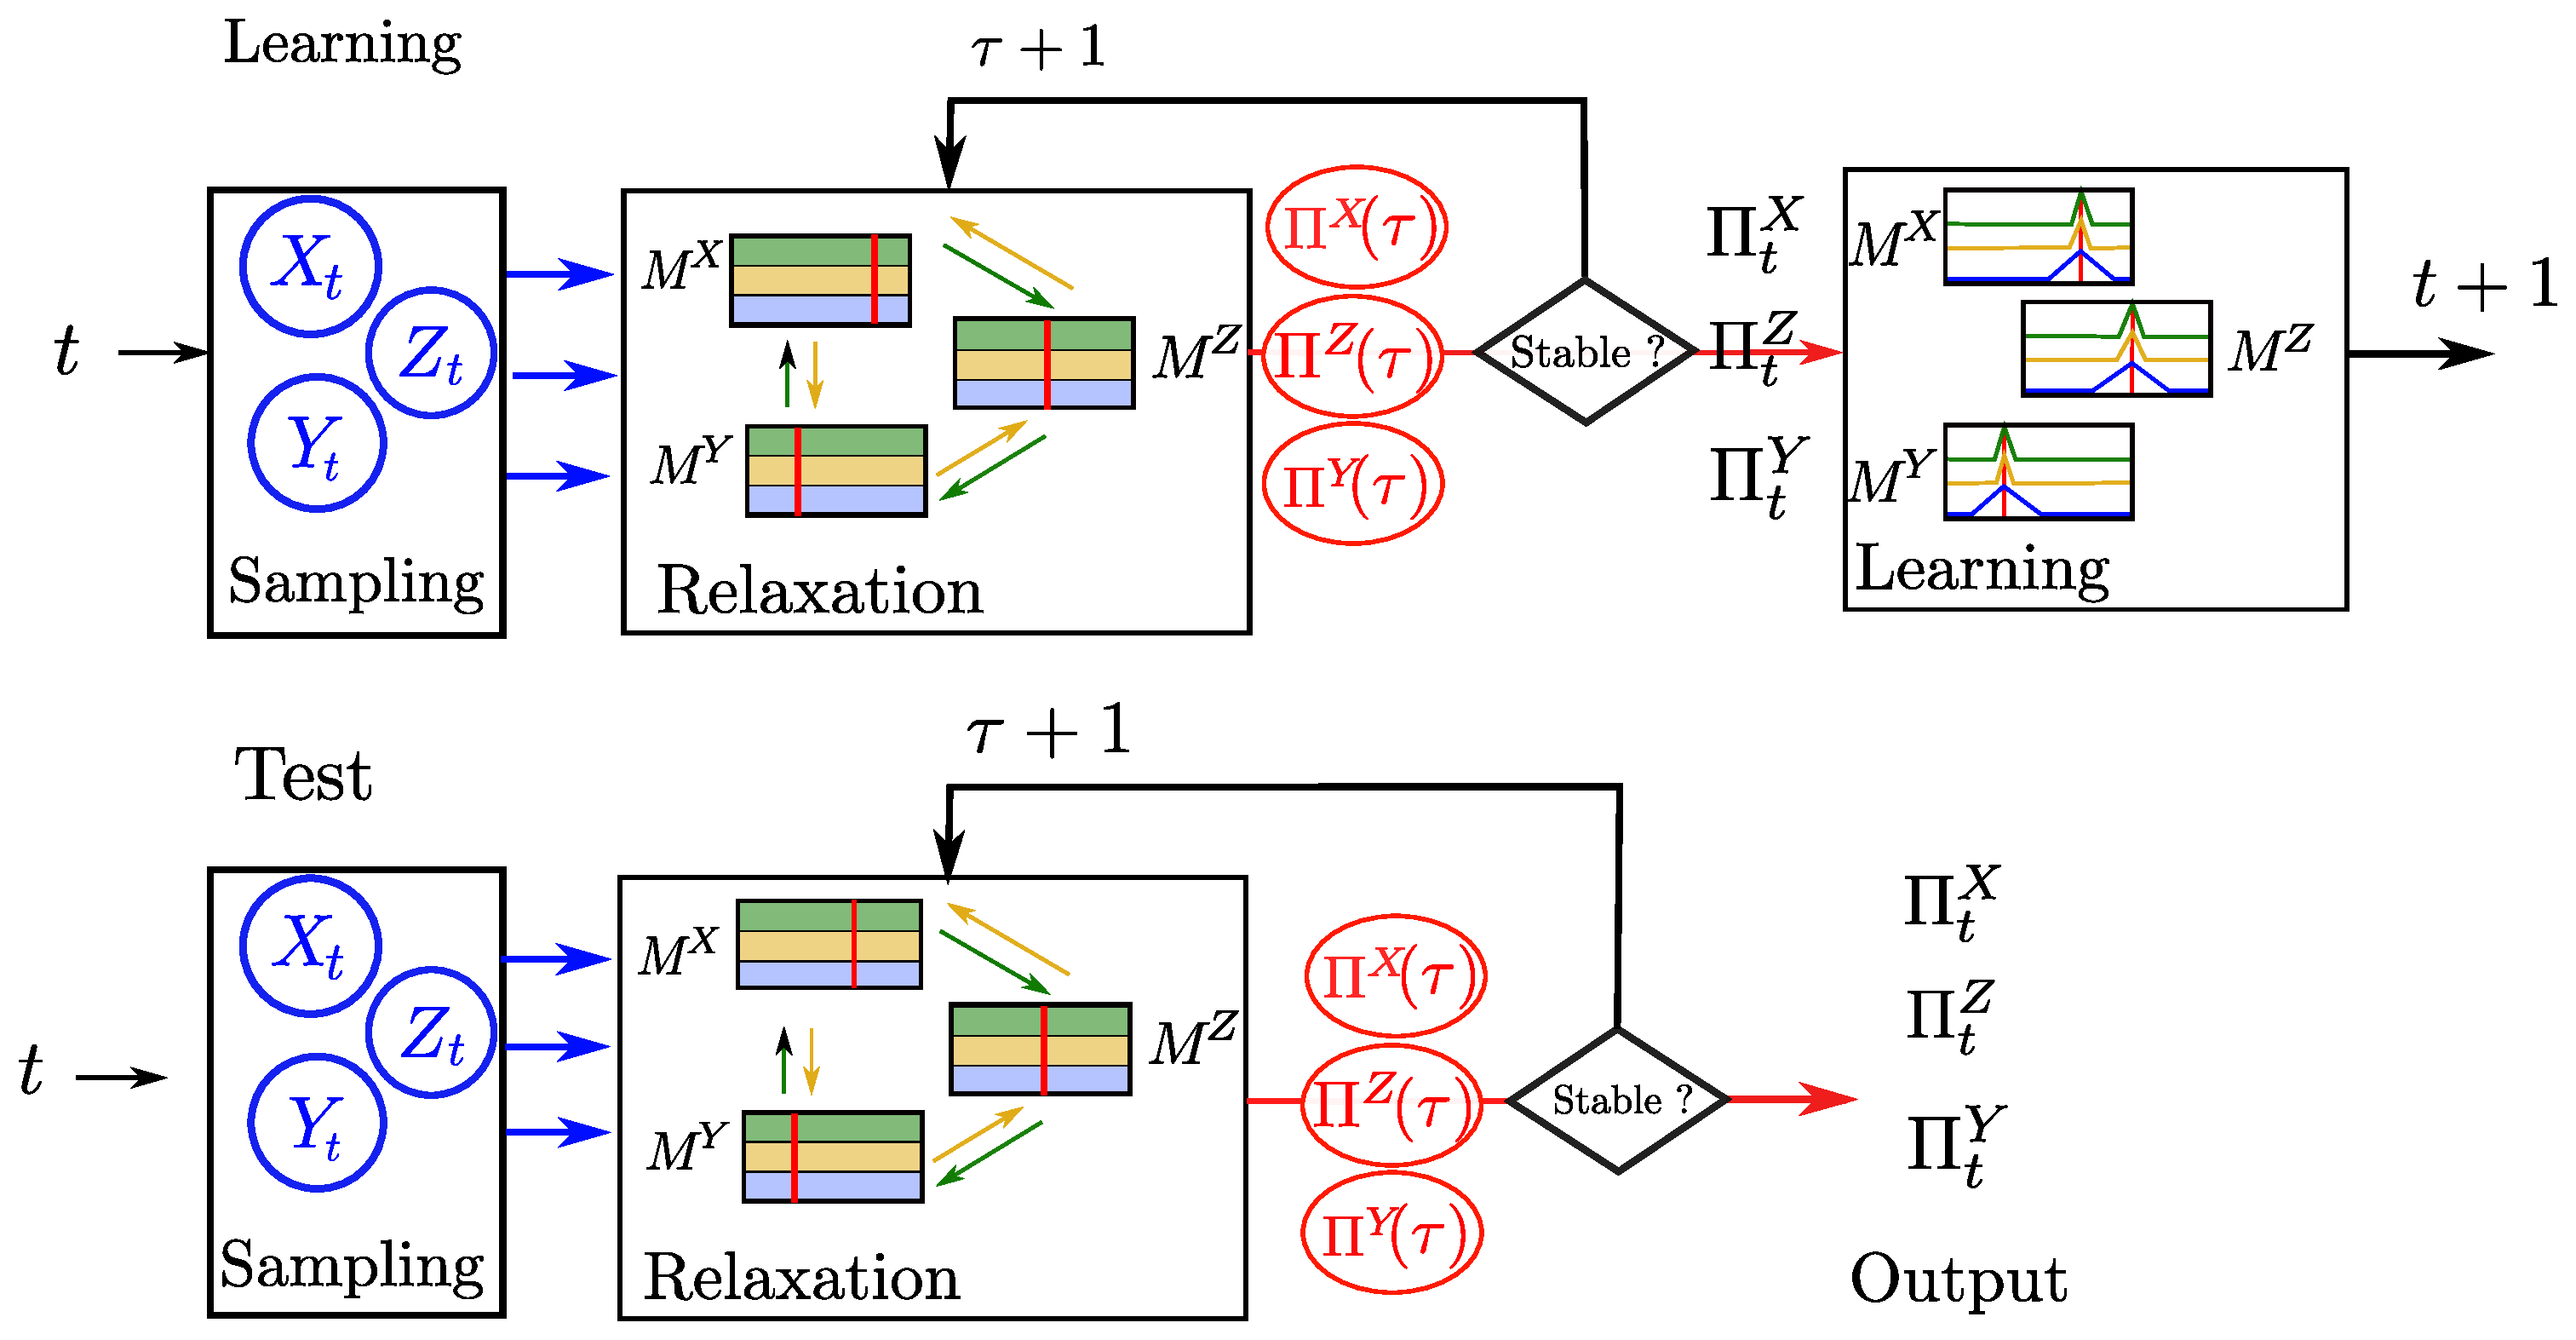
\includegraphics[width=0.7\textwidth]{learning_tests_nopred.pdf}
\caption{Schéma descriptif de l'apprentissage et des tests.}
\label{fig:flowchart}
\end{figure}


\section{Représentations graphiques}

On peut faire le choix de représenter le poids de la best matching unit par rapport à sa position. Cela donne une représentation similaire au tracé du poids de chaque prototype par rapport à sa position dans la carte.  Par contre, cette représentation fera la distinction entre les \emph{unités mortes de la cartes}, c'est à dire les unités qui ne sont jamais best matching unit et qui ne seront donc pas affichées, et les unités qui ont été BMU au moins une fois. Il s'agit d'une représentation qui prend en compte la façon de calculer le BMU.

La question de la répartition des valeurs d'une carte par rapport à la position de leur BMU va plus loin que les poids. On peut représenter, à partir d'un échantillon test, la dépendance de n'importe quelle variable par rapport à la position de la best matching unit correspondante. Nous détaillerons donc dans cette partie les tracés qui nous paraissent pertinents pour la compréhension de l'architecture CxSOM. 

\subsection{Représenter les entrées par rapport à une carte}

En première représentation, nous tracerons la valeur de l' entrée $\inpx\m{i}$ d'une carte par rapport à la position du BMU $\bmu\m{i}$. Cette représentation permet d'analyser la quantification des entrées par la carte. Ces tracés sont réalisables pour des cartes une et deux dimensions, et pour des entrées quelconques, que ce soient des réels ou des entrées de plus grandes dimension comme des images.
Pour mieux comprendre les relations entre entrées et plusieurs cartes, on tracera sur une même figure les entrées de ces cartes selon la position du BMU d'une des cartes.

Le tracé correspondant à l'expérience du cercle est présenté en figure~\ref{fig:inputs}. Représenter les entrées selon les positions des BMUs montre par exemple que lorsque les cartes sont connectées, les deux points rouge et bleu ayant la même valeur de $X$ ont un BMU différent dans la carte $X$, alors que leurs BMU seraient identiques si les cartes étaient indépendante. On peut donc, par cette représentation, associer des entrées à leur BMU. Cette représentation fait apparaître les zones mortes de chaque carte.

\begin{figure}
\begin{minipage}{0.27\textwidth}
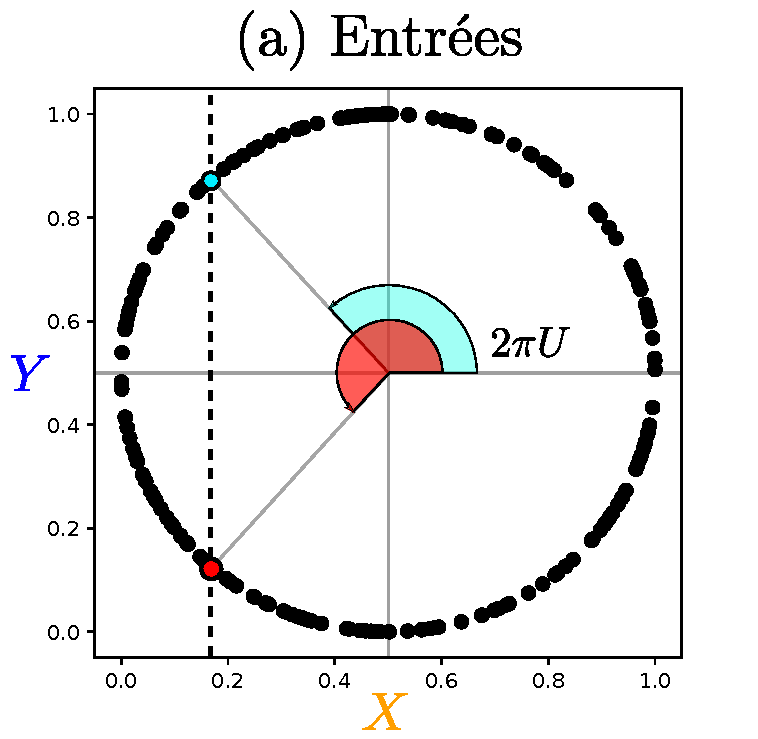
\includegraphics[width=\textwidth]{2som_inp.pdf}
\end{minipage}
\begin{minipage}{0.34\textwidth}
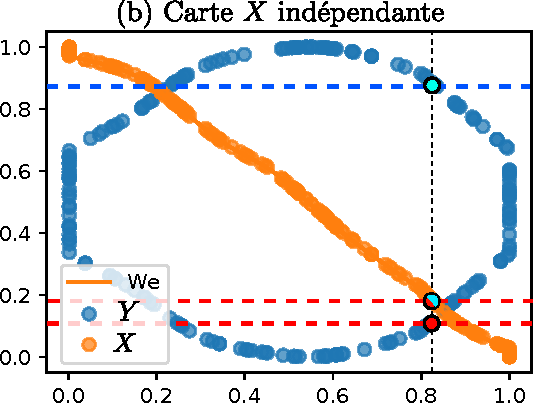
\includegraphics[width=\textwidth]{weights_2som_unco.pdf}
\end{minipage}
\begin{minipage}{0.38\textwidth}
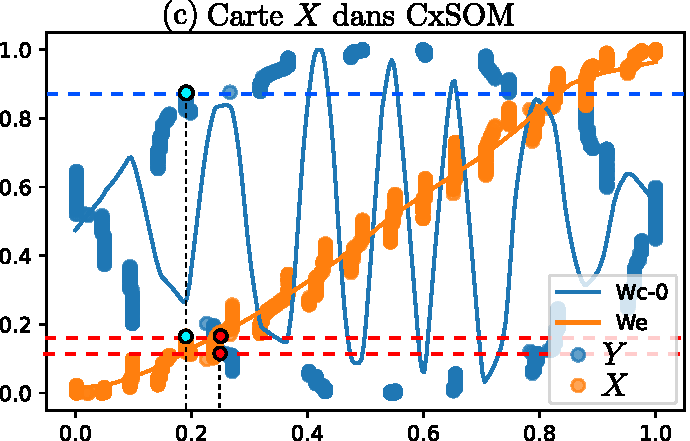
\includegraphics[width=\textwidth]{weights_2som.pdf}
\end{minipage}
\label{fig:inputs}
\caption{Représentation des entrées $X$,$Y$ d'une architecture de deux cartes relativement au BMU de la carte $X$ après apprentissage. Ces tracés mettent en valeur l'organisation des cartes, différentes dans le cas ou les cartes apprennent indépendemment leurs entrées~(b) ou connectées~(c). Les entrées correspondantes sont en figure~(a). Les points bleu et rouge reportés sur les tracés correspondent au même échantillon de test.}
\end{figure}

\subsection{Représentation de U par rapport au BMU}

Pour une, deux, trois entrées, les relations entre entrées se déduisent assez directement. Lorsqu'on augmente la dimension, il paraît pertinent de dégager des nouvelles valeurs qui représentent le modèle: il s'agit ici de la variable $U$. Cette variable cachée est en fait une représentation du modèle en dimension plus faible, par une transformation non linéaire. On peut alors tracer $U$ en fonction de la position $\bmu$ du BMU d'une carte pour représenter comment la position du BMU traduit la relation entre entrées. Le tracé en figure~\ref{fig:piu} montre $U$ comme une fonction de la position du BMU dans chaque carte, contrairement au cas ou les cartes ne sont pas connectées, tracé en figure~\ref{fig:piu_indep}. 

\begin{figure}
\begin{minipage}{0.45\textwidth}
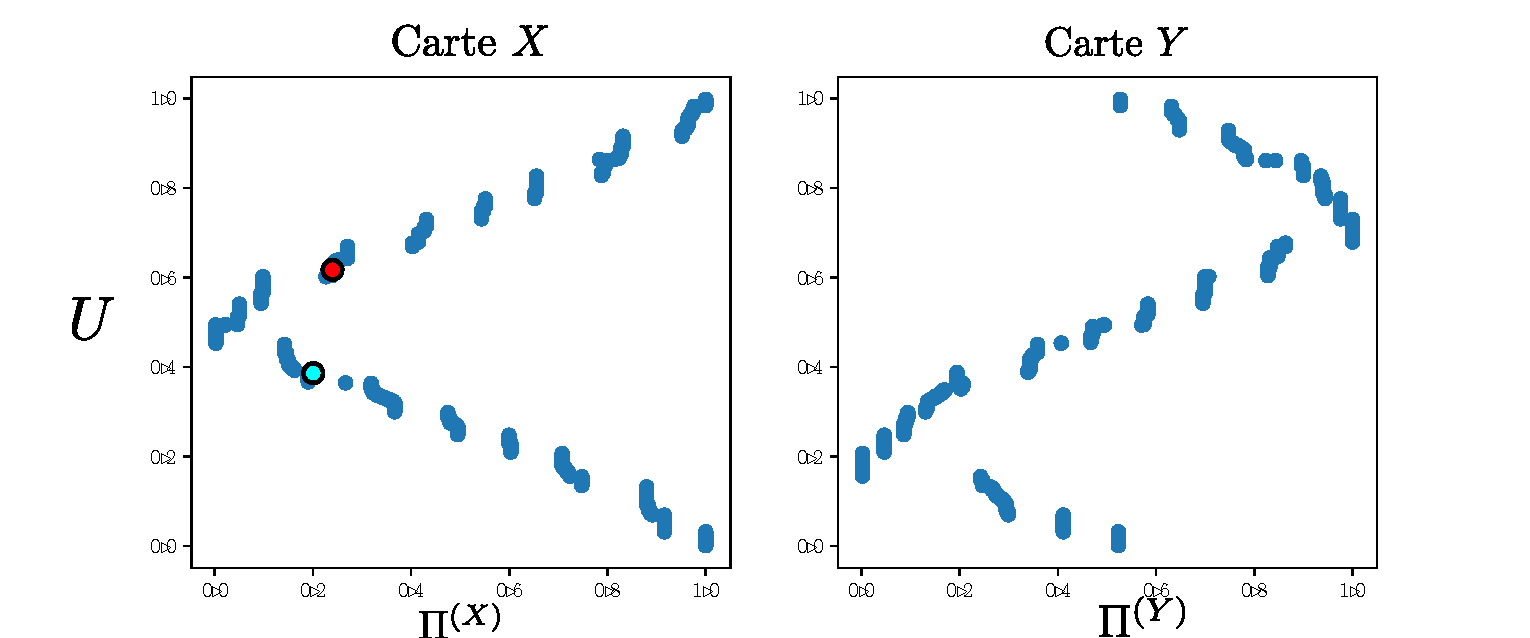
\includegraphics[width = \textwidth]{XU_YU.pdf}
\caption{Valeur de $U$ en fonction des valeurs du BMU $\bmu\m{i}$ dans chacune des cartes, pour des entrées prises sur le cercle. On voit que $U$ est une fonction de la position du BMU dans chaque carte, contrairement au cas ou les cartes apprendraient indépendamment sur les mêmes entrées, voir figure \ref{fig:piu_indep}.}
\label{fig:piu}
\end{minipage}
\hfill
\begin{minipage}{0.45\textwidth}
\centering
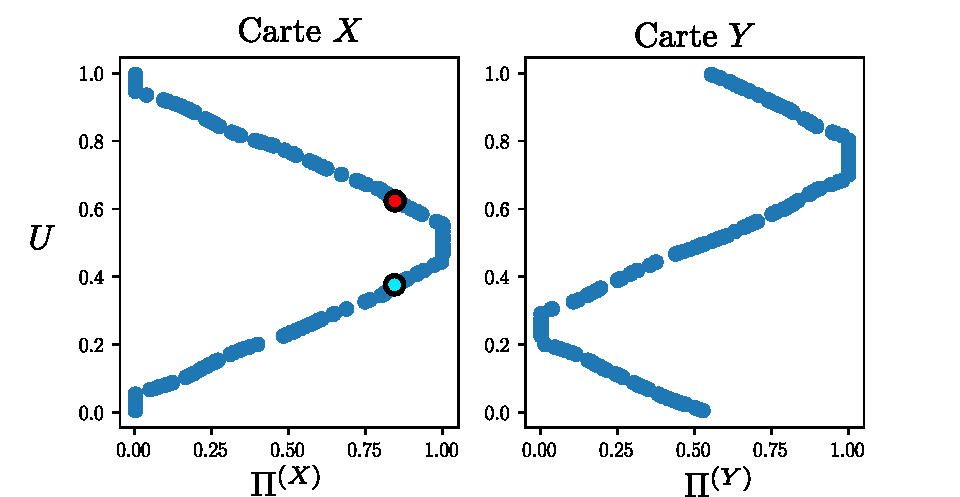
\includegraphics[width = \textwidth]{xu_yu_unco.pdf}
\caption{Pour l'échantillon de test, entrée sur un cercle, valeur de $U$ en fonction des valeurs du BMU $\bmu$ dans chacune des cartes, lorsque les cartes $M\m{X}$ et $M\m{Y}$ ne sont pas connectée. Chacune des cartes n'a aucune information de plus que celle portée par son entrée sur l'état global du système $U$, et $\bmu$ n'est donc pas une fonction de $U$ dans chaque carte. }
\label{fig:piu_indep}
\end{minipage}

\end{figure}


\subsection{Dépliement d'une carte en plusieurs dimensions}

Nous proposons une façon de représenter les poids d'une carte de Kohonen dans l'espace de toutes les entrées. Cette représentation est crée à partir des échantillons de test. Il s'agit de tracer les poids des BMUs dans l'espace de toutes les entrées: $(\w_e(\bmu\m{1}),\cdots,\w_e(\bmu\m{k}))$ dans l'espace en $k$ dimensions correspondant - $k$ correspondant ici à 2 ou 3 dimensions. Les échantillons sont ensuites reliés suivant l'ordre des positions dans \emph{une des cartes}. On obtient ainsi le \emph{dépliement} d'une carte de l'architecture dans l'espace multimodal à plusieurs dimensions. Un exemple de carte ainsi dépliée est présenté en figure~\ref{fig:distortion}.
\begin{figure}
\begin{minipage}{0.5\textwidth}
\centering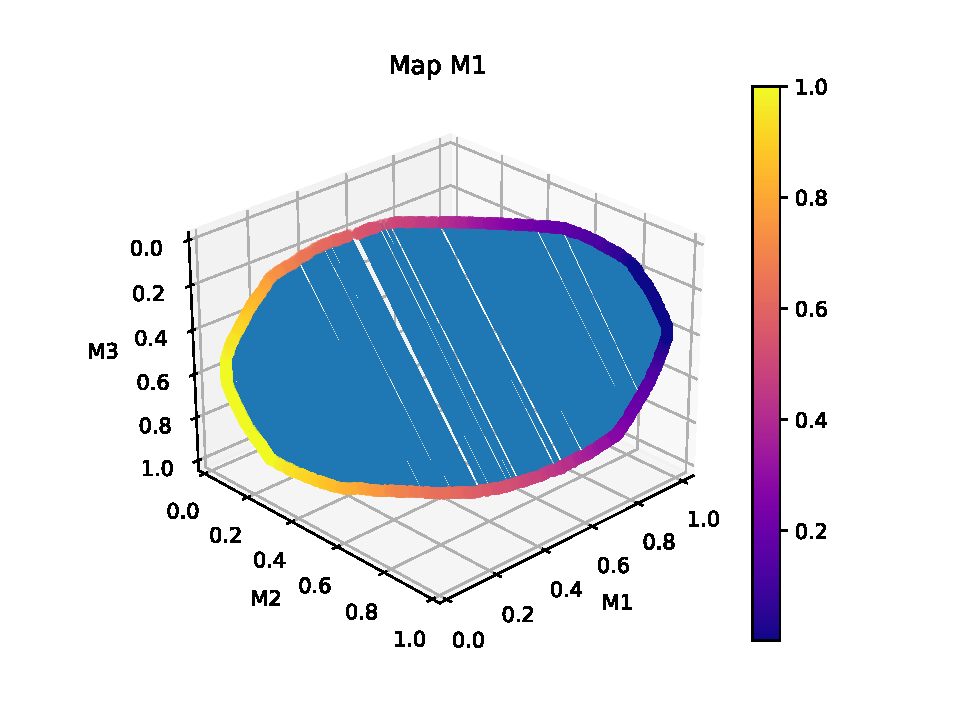
\includegraphics[width=0.8\textwidth]{unco3som}
\end{minipage}
\begin{minipage}{0.5\textwidth}
\centering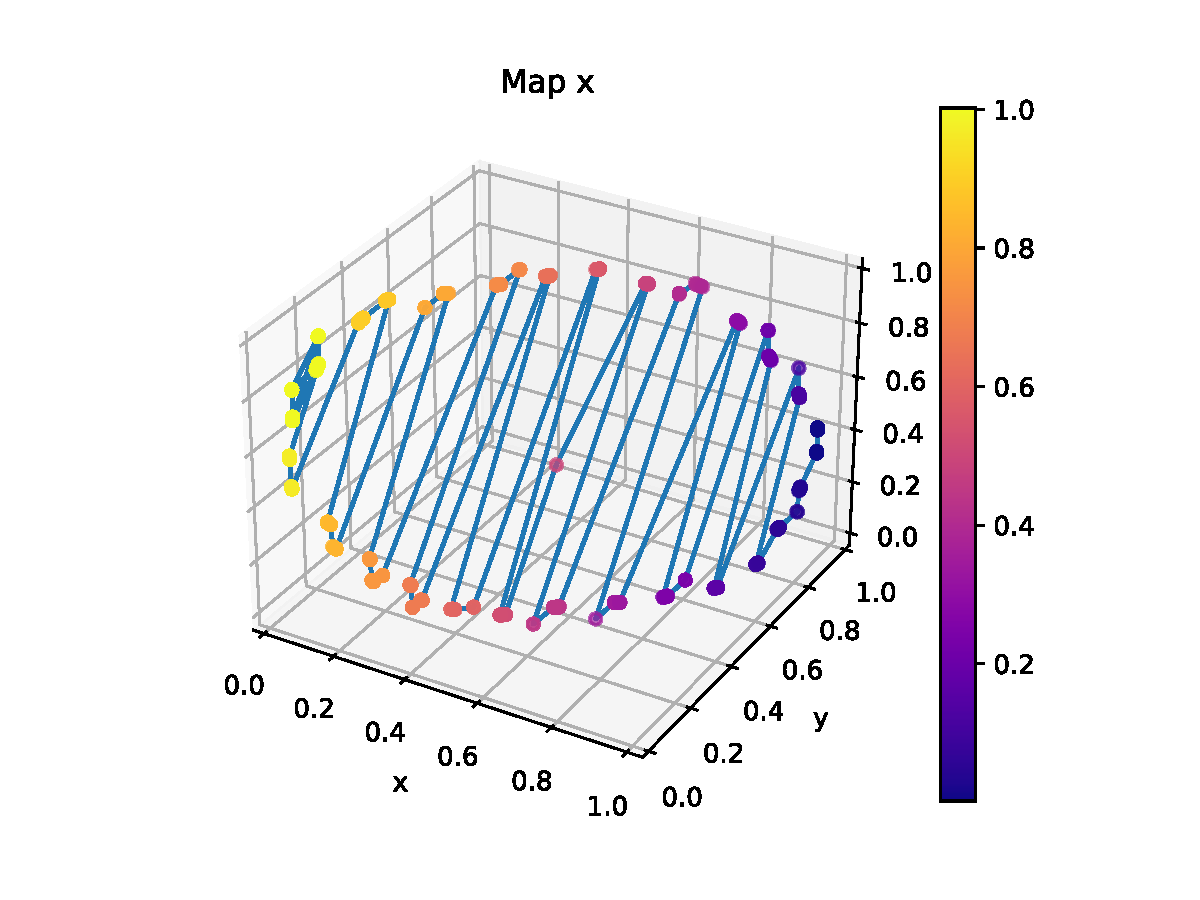
\includegraphics[width=0.8\textwidth]{disto_Mx}
\end{minipage}
\caption{Représentation des poids finaux de trois cartes prenant en entrée $X$,$Y$ et $Z$, reliés selon les positions de la carte $X$. A gauche, les cartes de l'architecture ont appris séparément sur les données. A droite, disposition lorsque les cartes ont été connectées au sein d'une architecture. Un échantillon de 1000 points a été utilisé pour les tracés.}
\label{fig:distortion}
\end{figure}

Ces figures sont équivalentes à tracer une carte dans l'espace de ses entrées: les poids des BMUs de l'échantillon sont les prototypes des cartes; seuls les poids des unités mortes ne sont pas représentés.
Cette représentation est limitée par la dimension des entrées, mais elle peut-être étendue: en plus grande dimension, il est possible de tracer le dépliement de la carte selon un sous-espace choisi de chacune des modalités, ou après réduction de dimension.
Par ailleurs, l'étude du comportement de cartes sur des données 3D s'inscrit dans la démarche de construction d'un modèle que nous suivons dans cette thèse. Leur visualisation est alors un élément clé dans la compréhension des comportements possibles de l'architecture. A partir de cette visualisation, on peut envisager de construire des indicateurs permettant l'analyse de l'architecture en dimension supérieure. 
Le second avantage de ces tracés est qu'il est possible de représenter graphiquement une carte qui ne prend pas d'entrée externe, ou de représenter une carte dans l'espace des poids d'autres cartes.

\section{Information mutuelle comme indicateur statistique}

L'étude de tout processus physique s'effectue par un ensemble signaux issus de capteurs. La théorie de l'information de Shannon \cite{Shannon1948AMT} apporte un modèle mathématique qui abstrait ces signaux et permet de les manipuler, les encoder, les décoder et quantifier l'apport ou perte d'information entre eux, en les utilisant en tant que distributions de probabilités.
Ce modèle mathématique puissant permet de s'abstraire de la nature des signaux pour s'intéresser à leurs relations. Comme son nom l'indique, la théorie de l'information s'appuie sur la notion fondamentale d'information portée par un symbole. Ensuite, cette information se décline en quantités qu'on calcule en fonction de ce qu'on veut mesurer: l'entropie d'une variable, comme l'information apportée par l'observation de la variable seule; l'entropie conditionnelle entre deux variables,l'information mutuelle entre deux variables ou un plus grand nombre. Ces mesures définissent une dépendance statistique générale, et ne dépendent pas du type de modèle ou de relation.

\draft{La théorie de l'information est non seulement applicable, mais en fait profondondément liée aux algorithmes l'apprentissage automatique~\cite{mackay2003information}. L'informatique prend sa source dans les travaux de recherche en la théorie de l'information au XXème siècle. L'apprentissage automatique en est un aspect.
Ces algorithmes cherchent en effet à apprendre un modèle, un signal liant des entrées à des sorties, ou des entrées entre elle. Ce modèle est un encodage du signal d'entrée. 
De son coté, la théorie de l'information apporte un langage fondamental pour quantifier la dépendance entre signaux, les encoder et les décoder. Les algorithmes d'apprentissage étant fondamentalement des encodeurs et des décodeurs, les quantités issues de la théorie de l'information ont donc une traduction directe dans les modèles d'apprentissage, et inversement.
D'ailleurs, de nombreux modèles d'apprentissage automatique se reposent directement sur des règles de calcul d'information pour encoder le signal d'entrée. On pense notamment aux approches bayésiennes de l'apprentissage qui estiment des distributions, et passent par des calculs d'information pour les estimer.}

Nous investiguerons dans cette partie comment quantifier l'apprentissage de l'architecture de cartes par des outils d'information. Bien que cette théorie soit un outil mathématique puissant, il s'agit d'un modèle s'appuyant sur les probabilités. L'estimation à partir de données est donc un élément clé et parfois limitant lorsqu'on cherche à utiliser des valeurs telles que l'entropie pour quantifier l'information au sein d'un système. Nous définirons donc dans cette partie des quantités à mesurer dans l'architecture de cartes, et chercherons à l'estimer.

\subsection{Information mutuelle et entropie}

Les notions d'\emph{entropie} et les valeurs qui en sont dérivées, telle que l'\emph{information mutuelle} entre des distributions, sont des notions fondamentales de la théorie de l'information de Shannon. Ces quantités donnent des informations concernant la distribution d'une variable aléatoire.
Les formules indiquées dans ce paragraphe concernent des variables aléatoire discrètes. 
L'entropie de Shannon d'une variable aléatoire $X$ à valeurs discrètes dans un ensemble $E_X$, de distribution $p(X)$, est notée $H(X)$ et définie par la formule : 
\begin{equation}
H(X) = - \sum_{x \in E_X}{p(x)\textrm{log}(p(x))}
\end{equation}

Elle se mesure en $bit/symbole$ lorsque le logarithme est en base 2, ce qui est généralement utilisé. 
L'entropie est une mesure de la quantité d'incertitude, ou de surprise, sur la valeur de la variable aléatoire $X$. Si la la distribution de probabilité de $X$ est concentrée autour d'un point, l'entropie est faible : lors d'une réalisation de $X$, l'observateur est \emph{plutôt certain} du résultat. En revanche, l'entropie est maximale lorsque lorsque $X$ suit une distribution de probabilité uniforme.
L'entropie s'interpète également comme la quantité moyenne d'information à fournir, en bits, pour coder la valeur que prend la variable $X$.
De la même manière, on peut définir l'entropie conjointe de deux variables, qui est l'entropie de leur distribution jointe, et l'entropie conditionnelle, qui est l'entropie de leurs distributions conditionnelles.

Outre les entropies jointes et conditionnelles, les relations statistques entre deux variables aléatoires $X,Y \in E_X,E_Y$ peuvent être mesurées par \emph{l'information mutuelle}. Elle se définit formellement par : 
\begin{equation}
 I(X,Y) = \sum_{x,y \in E_X,E_Y}{p(x,y)\textrm{log}(\frac{p(x,y)}{p(x)p(y)})}
\end{equation}
Cette valeur mesure la quantité d'information moyenne apportée par une réalisation de $X$ sur la réalisation de $Y$.

L'information mutuelle possède les propriété suivantes:
\begin{enumerate}
\item $I(X,Y) = 0 \Leftrightarrow \textrm{X et Y sont indépendantes}$. L'information mutuelle peut être vue une mesure de la distance entre la distribution jointe de $(X,Y)$, $p(X,Y)$ et la distribution dans laquelle les deux variables sont indépendantes, $p(X)p(Y)$.
\item Elle s'exprime à partir de l'entropie : $I(X,Y) = H(X) + H(Y) - H(X,Y) = H(X) - H(X|Y) = H(Y) - H(Y|X)$
\item Elle est symétrique : $I(X,Y) = I(Y,X)$
\item Pour toute fonction $f$, $I(X,Y) \geq I(X,f(Y)$. L'égalité est atteinte si et seulement si $f$ est \emph{bijective}.
\end{enumerate}


\subsection{Indicateur: coefficient d'incertitude.}

Lors de l'analyse de CxSOM, on s'interroge sur l'information que portent les positions des BMUs $\bmu$ d'une carte sur le modèle d'entrées. Les éléments de la carte ont été définis en terme de variables aléatoire; on peut donc utiliser l'information mutuelle comme une représentation de l'information portée par le BMU d'une carte sur le modèle. Le modèle est représenté par la variable $(X,Y,Z)$, mais aussi par $U$. $I(\bmu, U)$ est alors l'information moyenne que le BMU d'une carte porte sur $U$, donc sur le modèle, et $U$ sur le BMU. On souhaite cependant avoir un indicateur normalisé, qui permettrait, sur une échelle de 0 à 1, de quantifier à quel point un BMU porte de l'information sur $U$. On va donc normaliser l'information mutuelle $I(\bmu,U)$ par la valeur maximale qu'elle peut prendre dans notre carte.


Cette valeur maximale atteinte par $I(\bmu,U)$ est $H(U)$, atteinte lorsque $U$ est fonction de $\bmu$.
En effet, par construction, $\bmu$ est une fonction de $U$ dans une carte de Kohonen: l'algorithme est déterministe et une sortie est définie pour toute valeur de $U$. 
Par propriété de l'information mutuelle, pour toute fonction $f$ et variables $X,Y$, $I(X,f(Y)) \leq I(X,Y) $.
Donc, $I(U,\bmu) \leq I(U,U) = H(U)$
Cette valeur est atteinte si et seulement si $U$ et $\bmu$ sont en bijection, autrement dit, si et seulement si $U$ est aussi une fonction de $\bmu$.


Nous définissons donc un indicateur de la relation entre $U$ et un BMU comme:
\begin{equation}
UC(U|\bmu) = \frac{I(\bmu,U)}{H(U)}
\end{equation}
Ce coefficient n'est pas symétrique, et mesure donc l'information portée par le premier terme sur le second, relativement à la valeur maximale qu'elle peut prendre. Dans le cas des cartes CxSOM, $UC \in [0,1]$. Cette valeur rappelle le \emph{coefficient d'incertitude} entre $U$ et $\Pi$, ou $U$ de Theil \cite{Theil1961EconomicFA}.

%TODO : développer ce point : information portée par plus de variables !
%TODO : calculer et comparer les valeurs pour le cas du cercle.

 
Ce coefficient peut être élargi à plus de variables. On peut ainsi calculer $UC(U | (\bmu\m{1},\bmu\m{2},\bmu\m{3}))$ pour 3 cartes, en considérant la variable jointe $(\bmu\m{1},\bmu\m{2},\bmu\m{3})$. Plus largement, pour prouver qu'on a bien appris un modèle, on souhaite que $UC(U|\bmu\m{1},\cdots,\bmu\m{k})$ soit le plus proche possible de 1.

\comment{Qu'est ce que l'information portée par plusieurs variables représente dans le cas du cercle !}

\subsection{Estimation}
%TODO

\comment{ TODO :
Limitations : biais, variance (definition mathématique ?)
Traduction de ces limitations concrètement, notamment pour le calcul du rapport info/entropie : a quoi doit on faire attention ?
}

\comment{
On veut expliquer comment on s'y prend pour estimer le coefficient d'incertitude. On a plusieurs méthodes possible : estimation par binning et estimations par noyaux, par exemple Kraskov. L'estimation par noyaux est plus précise et limite la variance et le biais de l'estimateur, et sera plus fiable en plus grandes dimensions. ( préciser la source ???)
Si on trace l'évolution de l'info mutuelle pour 2 cartes connectées et non connectée, estimée en binning et Kraskov, on 
}

L'information mutuelle et l'entropie sont des grandeurs probabilistes. Elles sont définies à partir de la distribution des variables aléatoire. Lorsque qu'on ne connait pas les distributions, il est nécessaire d'estimer ces valeurs autrement. 
Une première façon d'estimer l'entropie et l'information mutuelle entre $X$ et $Y$ est d'estimer la distribution des variables $X$,$Y$ et leur distribution jointe $Z = (X,Y)$ en discrétisant l'espace par \emph{binning}, représenté en figure~\ref{fig:binning}. Les variables X et Y sont donc discrétisées en \emph{boîtes} de centres $x_k$ et $y_k$. La distribution de X est alors estimée par: 
$$P(X = x_i) = \frac{n_{xi}}{N} $$, où $n_{xi}$ est le nombre d'échantillons de X tombant dans la boîte de valeur $x_i$ et $N$ le nombre de points. Le même procédé est réalisé pour $Y$ et $Z = (X,Y)$.
L'information mutuelle par binning est calculée à partir de ces distributions discrètes.
\draft{Lorsque la dimension des variables est faible (typiquement 1D), l'estimateur est ?? (fiable ?? comment)}
Des termes de corrections peuvent être apportés. La précision de l'estimation peut être améliorée en choisissant des tailles de boîtes variables. Cependant, lorsque la dimension augmente, le nombre d'échantillon disponibles doit augmenter exponentiellement avec la dimension des variables pour éviter le phénomène de "boîtes vides": à cause de la dispersion des données, de nombreuses boîte $(x_j,y_i)$ ne contiendront pas de points alors qu'elles auraient du en contenir selon leur distribution; l'estimation de la probabilité en ce point sera donc nulle, et l'indicateur faussé. 

Un autre estimateur que le binning est l'estimation par noyaux de Kraskov \cite{2004kraskov}. Cet estimeur passe par une estimation diecte de l'entropie au lieu des densités de probabilités. Le découpage de l'espace se fait en recherchant, pour un couple $(X,Y)$ les k plus proches voisins. Une information mutuelle locale est calculée dans cette zone de l'espace, suivant une formule permettant d'approximer les différences de logarithme par la fonction digamma $\psi$ : 
$$i_j(X,Y) = \psi(k) - \psi(n_{x_j} + 1) - \psi(n_{y_j} +1) + \psi(N)$$
Cette information mutuelle locale est ensuite moyennée sur l'ensemble des points: 
$$\hat{I}(X,Y) = \psi(k) - \langle\psi(n_{x_j} + 1) + \psi(n_{y_j} +1)\rangle + \psi(N)$$
Cet estimateur est meilleur que le binning, car il ?? 
Il permet également d'éviter les boîtes vides du binning, car on n'explorera que l'espace des points. Il semble donc préférable d'utiliser cet estimateur en plus grande dimension.
L'estimation de $UC(X|Y)$ nécessite d'estimer $I(X,Y)$ et $H(Y)$ : leur estimation doit être réalisée dans les mêmes conditions.

L'information mutuelle et l'entropie étant des quantités fondamentales en théorie de l'information, il existe de nombreuses méthodes d'estimations de ces valeurs malgré la difficulté qu'elle pose. On peut notamment citer~\cite{Belghazi2018MutualIN}, qui utilise une approche neuronale pour estimer l'information mutuelle. Ainsi, l'utilisation du coefficient d'incertitude comme indicateur semble réutilisable pour des données de plus grande dimension ou pour plus de cartes, quitte à utiliser des méthode d'estimations plus élaborées. 

\begin{figure}
\begin{minipage}{0.45\textwidth}
\centering
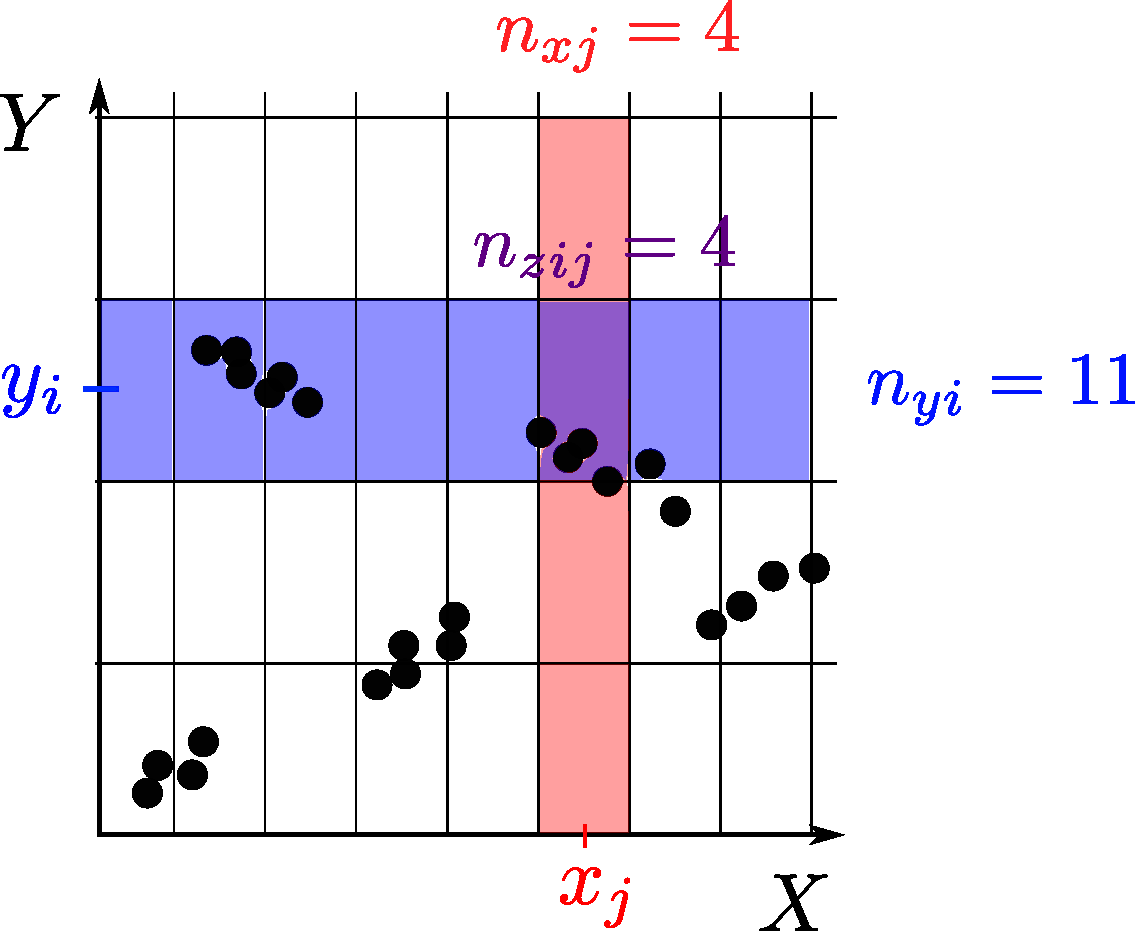
\includegraphics[width=0.9\textwidth]{boxes}
\caption{Procédé de binning pour estimer les distributions des variables $X$ et $Y$. Les distributions sont estimées à partir de $n_{xj}$, $n_{yi}$ et $n_z{ij}$, puis les valeurs de $H$ et $I$ calculées.}
\label{fig:binning} 
\end{minipage}
\hfill
\begin{minipage}{0.45\textwidth}
\centering
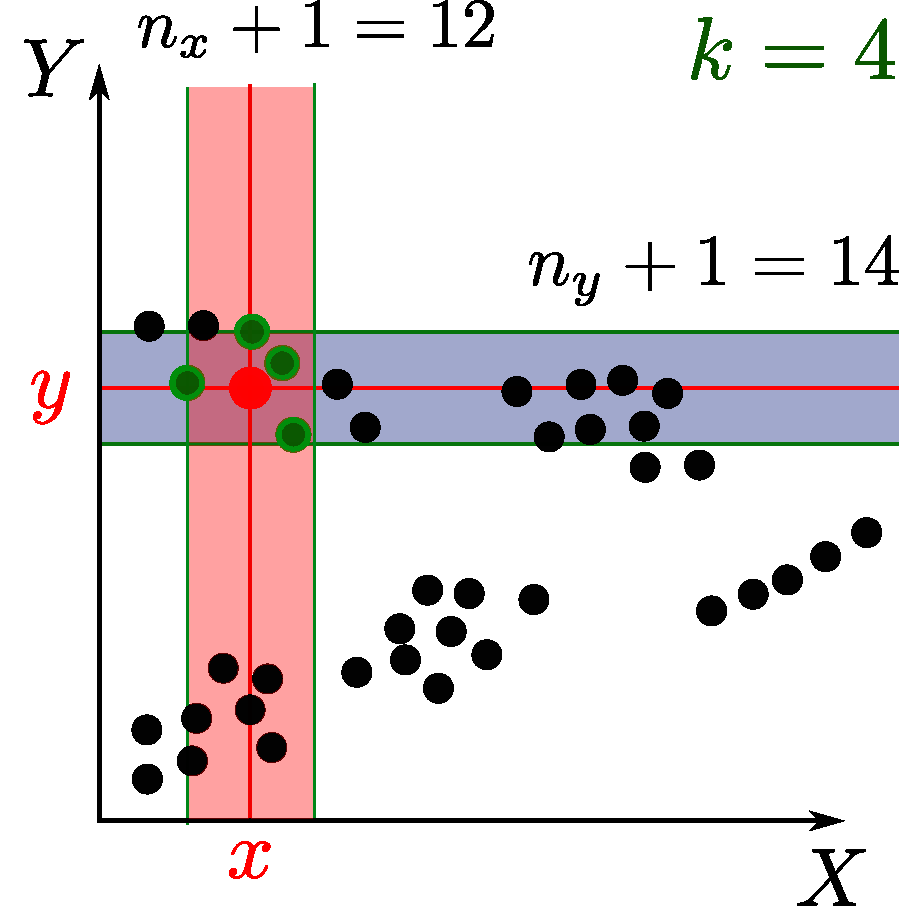
\includegraphics[width=0.7\textwidth]{kraskov}
\caption{Découpage en KNN de Kraskov pour estimer l'entropie et l'information mutuelle des variables $X$ et $Y$. Les plus proches voisins du point rouge sont trouvés, en vert, et le processus est répété sur tous les points. Les valeurs de $n_x$ et $n_y$ permettent d'estimer directement l'entropie.}
\label{fig:kraskov}
\end{minipage}
\end{figure}

%\begin{figure}
%\centering
%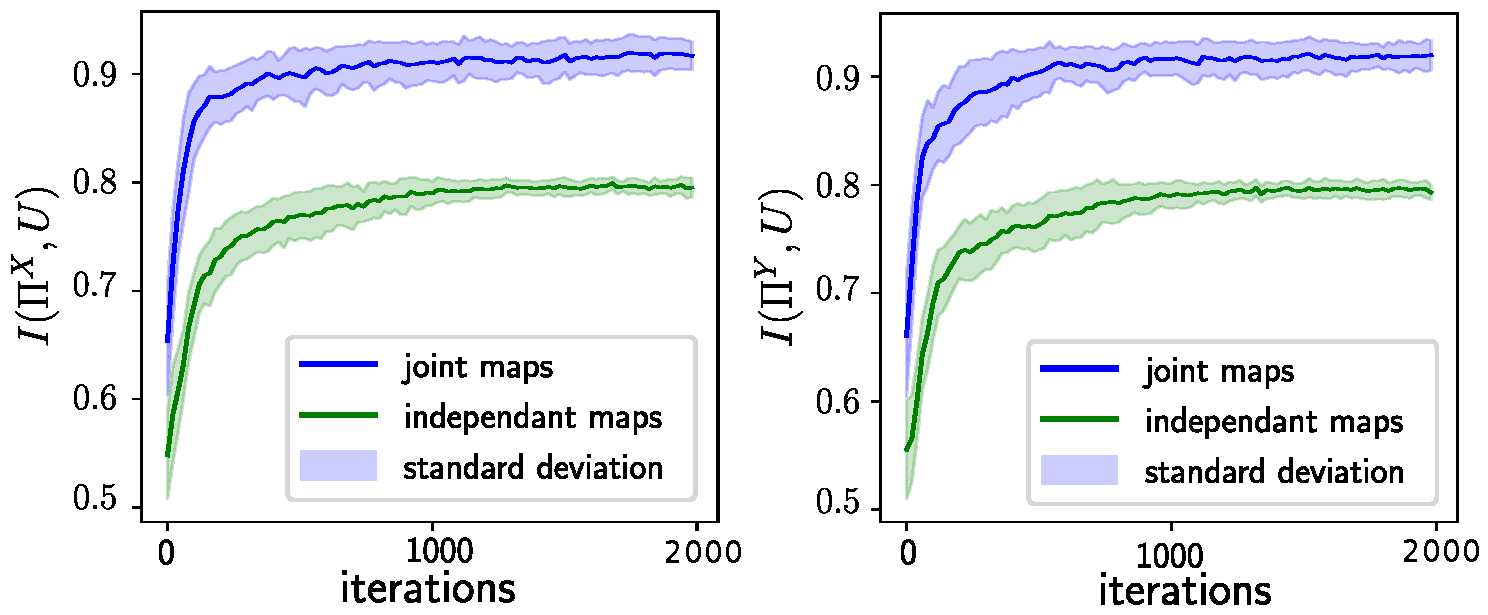
\includegraphics[width=\textwidth]{mutual_info_evol.pdf}
%\caption{Evolution de l'indicateur relatif à l'information mutuelle entre $\Pi$ et $U$ dans chaque carte au cours de l'apprentissage. Cet indicateur est comparé à celui calculé dans le cas ou les cartes apprennent séparément.}
%\label{fig:im} 
%\end{figure}
\draft{
\subsection{Ration de Corrélation}
Un autre indicateur
}

\subsection{Perspectives}

\subsubsection{Erreurs sur les données bruitées}

Le coefficient d'incertitude mesure une forte relation statistique entre les données. Cela mesure bien ce qu'on apprend entre cartes; cependant, il ne prend pas en compte l'aspect continu des variables. Ainsi, prenons une distribution $X$ quelconque et deux distributions $Y_1$ et $Y_2$, telles que représentées en figure~\ref{fig:exemple-limite}.$Y_1$ et $X$ ne sont pas en bijection, mais ont une forte dépendance statistique: lorsqu'on connait la valeur de $X$, seules deux valeurs sont possibles pour $Y_1$.
$Y_2$ et $X$ ne sont pas en bijection, mais en sont proches: leur relation est en fait une bijection, mais avec du bruit. Lorsqu'on analyse des données de CxSOM, les entrées sont généralement bruitées, tout comme les sorties. Par contre, on voudrait privilégier l'existence d'une dépendance forte entre entrées et sorties qui ne tiennent pas compte de ce bruit. Or, dans l'exemple cité, $UC(Y_1|X) = 0.6$ et $UC(Y_2|X) = 0.4$. L'indicateur n'est donc pas complètement approprié dans le cas de variables avec bruit.

\begin{figure}
\centering
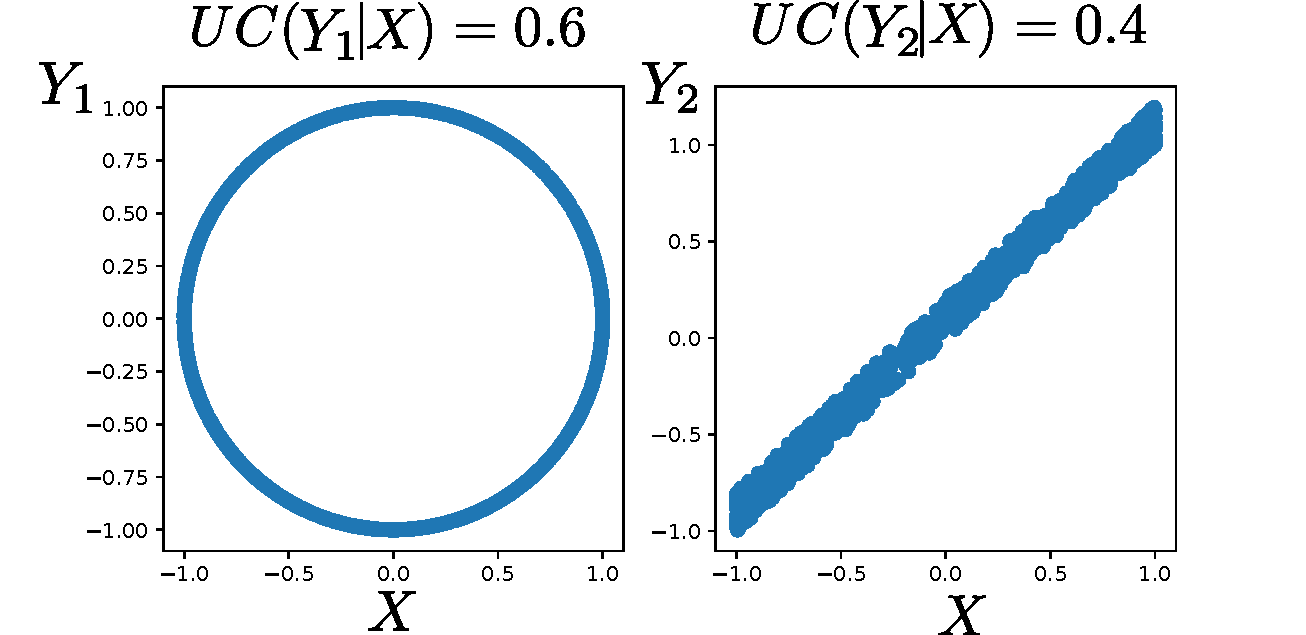
\includegraphics[width=0.7\textwidth]{exemple_limite.pdf}
\caption{Pour ces deux distributions $X$ et $Y$, le coefficient d'incertitude mesure une meilleure dépendance statistique dans le premier cas que le second. On voudrait au contraire privilégier le score de la seconde relation.}
\label{fig:exemple-limite}
\end{figure}

\subsubsection{Perspectives d'amélioration}

\comment{Correlation ration : mesure de dépendance fonctionnelle
Débruitage de l'IM : répétition de l'expérience et moyenne ?}

\subsubsection{Discussion}

Le ration de corrélation traduit mieux que le coefficient d'incertitude la dépendance fonctionnelle entre le modèle et le BMU. Cependant, à l'inverse de l'information mutuelle, une relation non fonctionnelle mais précise (telle que l'exemple du cercle de la figure~\ref{fig:exemple-limite}) entre les variables aura un score très faible. Ce n'est pas non plus voulu. 

Il semble que l'information mutuelle reste le moyen le plus prometteur et le plus général de mesurer la relation entre les éléments des cartes. Dans le cas une dimension, on observe qu'on veut tendre vers U fonction du BMU; on connait mal le comportement recherché en dimension plus grande (cartes 2D, entrées de grande dimension). L'information mutuelle laisse donc l'opportunité à plus d'états d'organisation des cartes de l'architecture d'avoir un bon score. La meilleure perspective serait donc de pouvoir calculer le coefficient d'incertitude sur des échantillons provenant de données non bruitées, ou de pouvoir séparer le bruit des données lors du calcul du coefficient.
Dans cette optique, l'estimateur par binning permet de réduire l'effet du bruit, en choisissant correctement les tailles de boîtes. L'utilisation du binning versus Kraskov reste donc à discuter.
Dans le cas ou le modèle d'entrée est connu, calculer les réponses des cartes sur des jeux de données non bruitées générées artificiellement, après apprentissage sur un jeu de données réelles et bruitée, est une solution. Si le modèle n'est pas connu, des méthodes statistique de réduction de bruit peuvent être imaginées. 

\draft{
\section{Prédiction d'entrée}

Au sein d'une architecture de cartes, il est possible de ne pas présenter à une ou plusieurs cartes de l'architecture leur entrée externe $\inpx\m{i}$. Dans ce cas, une best matching unit peut quand même être calculée par leurs entrées contextuelles. Le poids de cette best matching unit peut alors être vu comme une prédiction de l'entrée manquante. Cette capacité de prédiction peut être à la fois vue comme une application possible de l'architecture, mais aussi comme une façon de représenter \emph{ce que les autre cartes connaissent d'une autre}. Tracer les prédictions d'une carte est donc un indicateur de la façon dont une architecture a appris des relations. 


\comment{
2 parties dans estimation/perspectives : 
d'une part, questionnement sur l'estimation des données bruitées par exemple - pas besoin de proposer des solutions si elles ne sont pas testées ? 
Et parler de l'estimation en grande dimension : ce n'est pas forcément le pb ici. Donc pas la peine...
}
}
\chapter{Analyse de l'organisation de CxSOM}\label{chap:analyse}
\graphicspath{{04-Analyse/}}
\minitoc

\section{Identification des comportements de blocs élémentaires de cartes}

Cette thèse s'inscrit dans une démarche expériementale d'analyse d'un système complexe.
Nous avons proposé un modèle de connexions de cartes auto-organisatrices au sein d'une architecture complète.
Ce modèle s'appuie sur des modèles de connexions entre cartes existant dans la littérature, utilisés notamment dans le cadre des cartes récurrentes: la transmission de la position du BMU entre cartes.
La démarche expérimentale est constructive: nous proposons un modèle qui semble pertinent au regard des résultats existants dans la littératures, sur des problèmes similaires que sont les cartes récurrentes. En effet, la transmission de contexte entre carte est un problème partagé par les modèles utilisés en traitement de séquence et en mémoire associative. Nous cherchons ensuite à évaluer la pertinence du modèle et identifier des comportements.

Nous avons présenté ce modèle et les méthodes de représentations sur lesquelles nous nous appuierons. L'expérience présentée en exemple a permis d'identifier quelques comportements élémentaires émergeant des connexions entre carte. Notamment, nous avons observé que les poids contextuels s'organisent de façon à ce qu'une carte différencie son BMU en fonction de son entrée externe et de son entrée contextuelle. 
Dans ce chapitre, nous analyserons ces comportements plus en détail, et identifierons les comportements \emph{systémiques} émergeant d'une architecture simple à deux et trois cartes.

\subsection{Auto-organisation émergeant d'architectures de deux et trois cartes}

Une architecture de cartes est un système complexe. 
Dans une logique de construction d'architecture, nous voulons d'abord identifier des comportements collectifs de cartes qui pourraient être intéressants dans l'apprentissage de données multimodales.
Nous avons choisi d'identifier ces comportements collectifs sur des petites architectures de deux et trois cartes en une dimension. Ces architectures sont représentables graphiquement.

Nous utiliserons la cartographie des entrées en fonction des BMUs dans deux dispositions d'entrées.
Dans toutes les dispositions, les modalités sont les coordonnées d'un point.
Nous considérerons des entrées tirées sur un cercle en deux et trois dimensions.
Dans cette disposition, chaque abcsisse $x$ correspond à deux valeurs de $y$, et inversement.
Dans cette disposition, nous ajoutons un bruit: le cercle sera en fait un anneau. Nous souhaitons ainsi évaluer si les cartes sont résistantes au bruit d'entrée et apprennent une représentation de la structure débruitée.
Nous étudierons également une disposition d'entrée prise sur l'ensemble du carré unité. Cette disposition d'entrée permet d'étudier comment une carte se comporte dans le cas ou il n'existe pas de relation entre les entrées.

Chaque expérience se déroule sur

Analysons d'abord la forme des poids contextuels de $M\m{1}$, que nous avions tracés en figure~\ref{fig:weights} sans les commenter. Les poids externes, en orange, présentent une disposition similaire à ceux observés dans la carte classique (b). Les poids contextuels, en bleu, présentent une forme de vagues, avec 7 valeurs de maximum allant de 0.5 à 1, et 6 minimum allant de 0.5 à 0.1. Ces maximum et minimum sont répartis en zones de taille équivalente sur la carte. 

Lorsqu'on s'intéresse au tracés des échantillons, on remarque d'abord que les positions dans la carte $M\m{1}$ se répartissent en zones étant BMUs et zones mortes, dans lesquelles aucune entrée n'a gagné. C'est une première différence avec la carte indépendante, pour laquelle toutes les positions gagneront pour des entrées. Les zones dans lesquelles il y a des BMUs correspondent aux extremum des poids contextuels et leurs alentours. C'est un phénomène inhabituel pour une carte de Kohonen. Les entrées $\inpx\m{1}$, dans la carte classique (b), correspondent à la courbe de poids externe: la valeur du poids du gagnant est toujours très proche de la valeur de l'entrée. Dans la carte $M\m{1}$, les entrées externes $\inpx\m{1}$ orange sont proches de la courbe de poids externes, mais avec plus d'erreur de quantification.
Les deux points rouge et bleu ayant la même valeur de $x$ ont un BMU différent dans la carte $M\m{1}$, alors que ces deux échantillons ont le même BMU dans la carte apprenant indépendamment sur les valeurs de $x$. Ainsi, la carte connectée au sein de CxSOM différencie les échantillons en fonction de non seulement leur entrée externe, mais aussi de l'entrée de l'autre carte de l'architecture. La plage de valeurs des $\inpx\m{1}$ gagnant dans un des zones recoupe les plages de valeurs gagnant dans les zones situées à gauche et à droite. Par exemple, la zone dans laquelle l'échantillon rouge gagne, autour de $\bmu\m{1} = 0.25$. La partie des entrées située en dessous de la courbe de poids externe recoupe les valeurs d'entrées gagnant dans la zone précédente; la partie située au dessous de la courbe de poids externe recoupe des valeurs gagnant dans la partie suivante. Pour une entrée externe, le choix de la zone de BMU dans laquelle elle gagnera dépend alors de l'entrée contextuelle. 


Dans la carte $M\m{1}$, une unité se spécialise donc par rapport aux deux entrées et non pas une seule comme dans la carte indépendante: les entrées externes et l'entrée contextuelles. C'est bien ce à quoi on s'attendait en ayant deux couches de poids. Ce qui est intéressant est que cette différenciation est réalisée par la répartition des unités en un nombre fini de zones distinctes. Dans chaque zone, les unités sont BMUs pour un segment de valeurs d'entrée externe et contextuelles. Au sein d'une zone, la répartition des entrées externe selon le BMUs est ordonnée, comme ce serait le cas dans une carte auto-organisatrice classique. Le comportement de la carte au sein d'une zone reste donc similaire à celui d'une carte classique.

Deux zones adjacentes correspondent par ailleurs à des segments de valeur d'entrée en partie superposés, et des segments de valeurs d'entrées contextuelles différentes. Il s'agit d'une deuxième échelle d'organisation, qui garde également l'aspect ordonné d'une carte classique. Ces zones sont créées par auto-organisation; aucun paramètre de la carte n'a été modifié pendant l'apprentissage pour former ces zones, et le nombre d'unités allouées par auto-organisation dans chaque zone est à peu près égal. La carte agit un peu comme une base de données structurée avec des indices primaires et des indices secondaires pour chaque neurone, l'indice primaire étant la zone de la carte, et l'indice secondaire la position dans cette zone.



\begin{itemize}
	\item 
\end{itemize}


\begin{figure}
	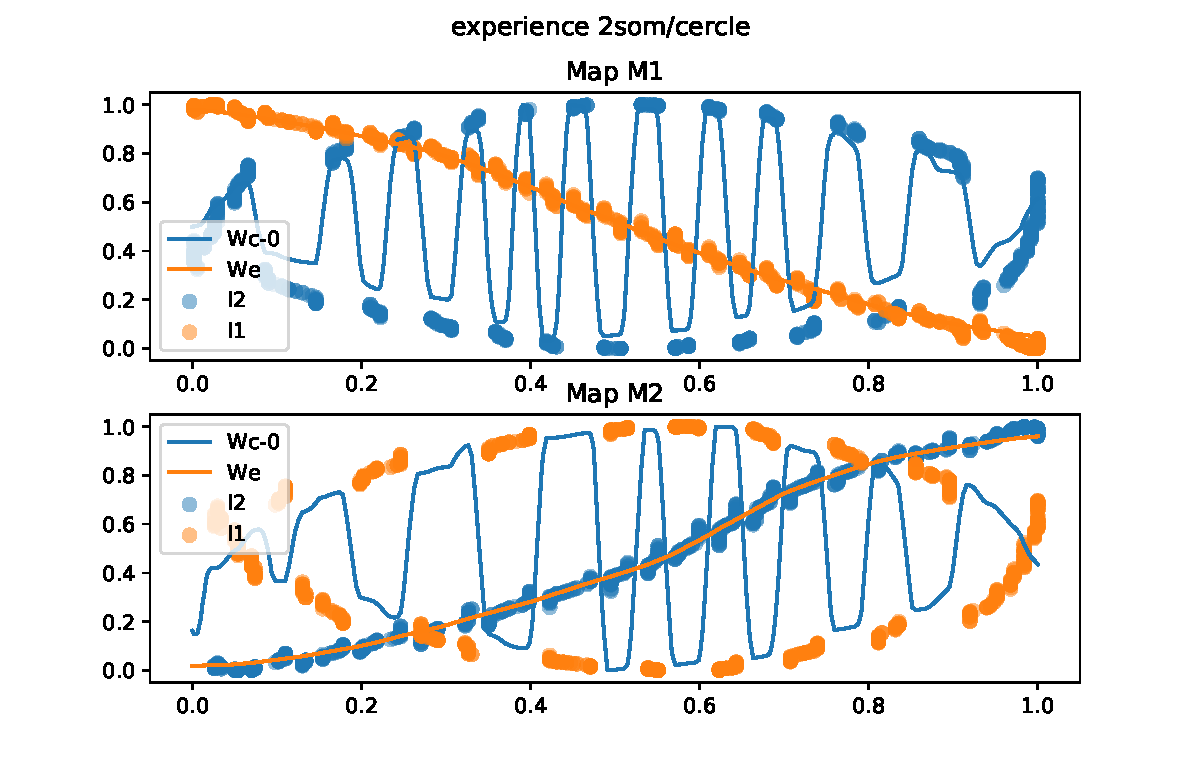
\includegraphics[width=0.7\textwidth]{2som_cercle_w.pdf}
\end{figure}

\begin{figure}
	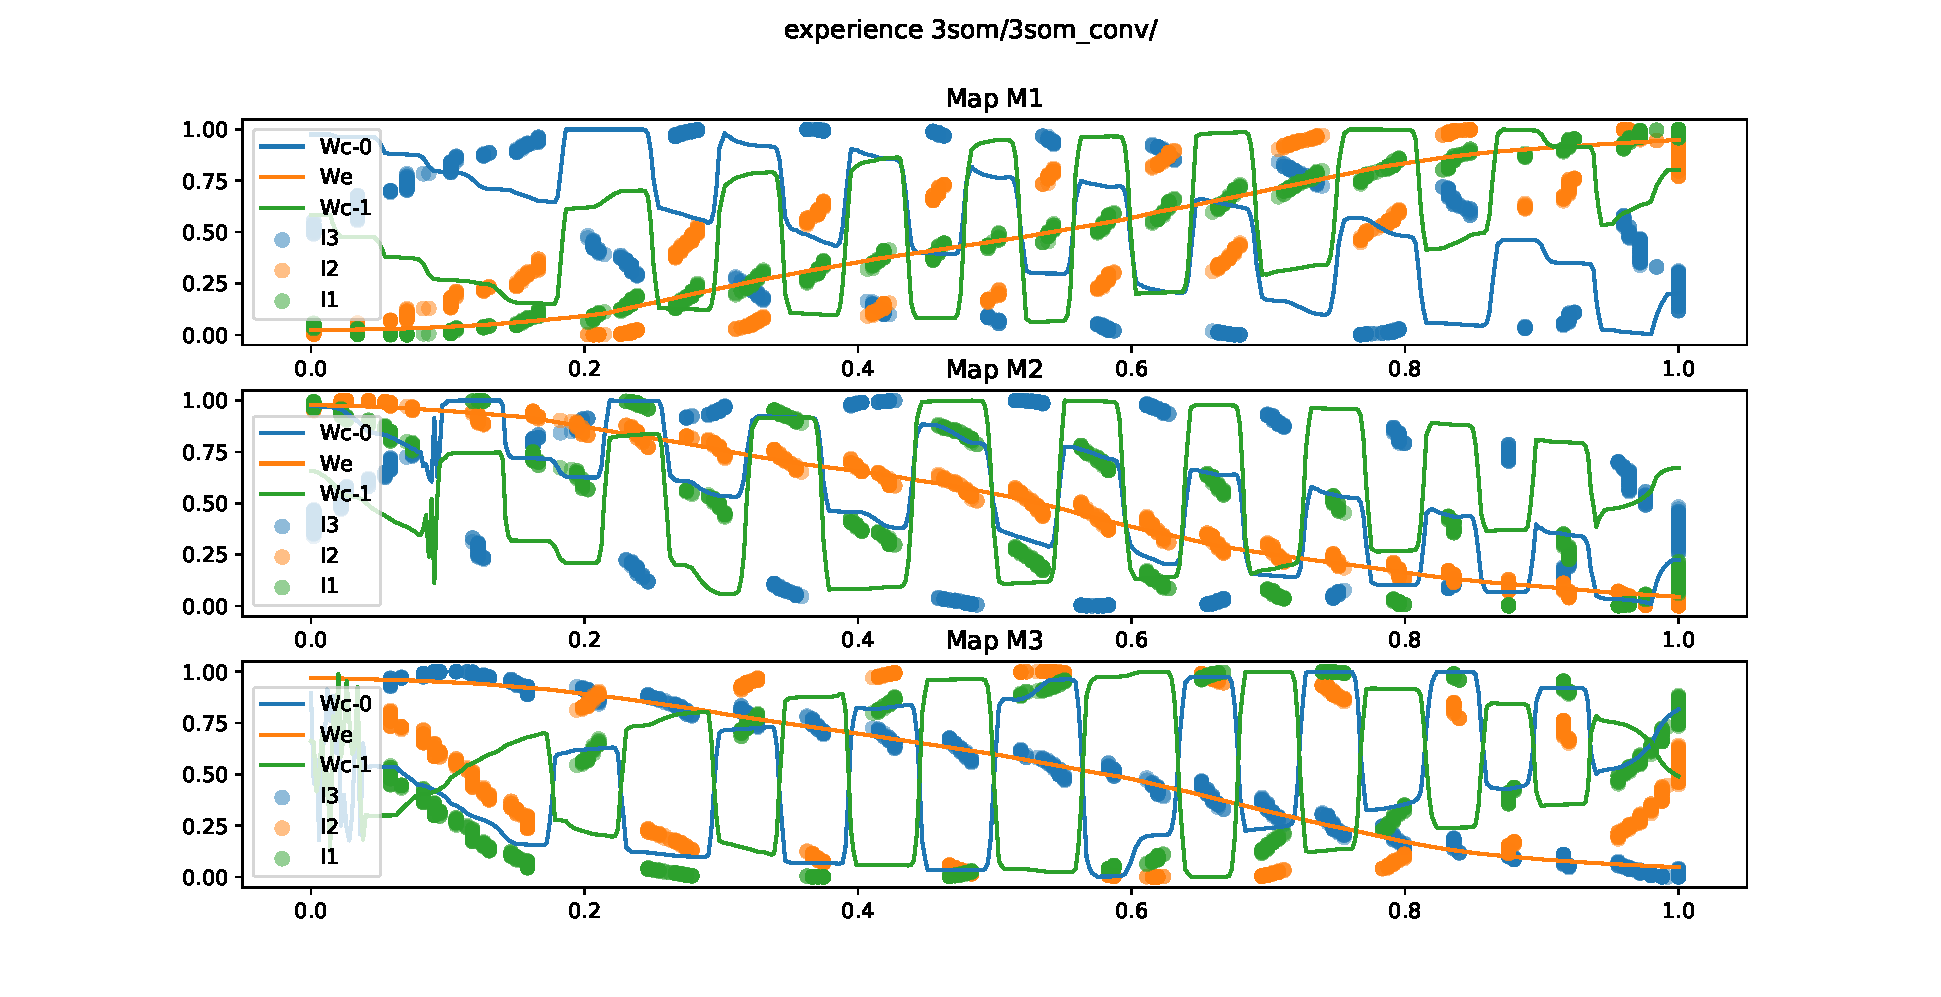
\includegraphics[width=0.7\textwidth]{3som_cercle_w.pdf}
\end{figure}

\begin{figure}
	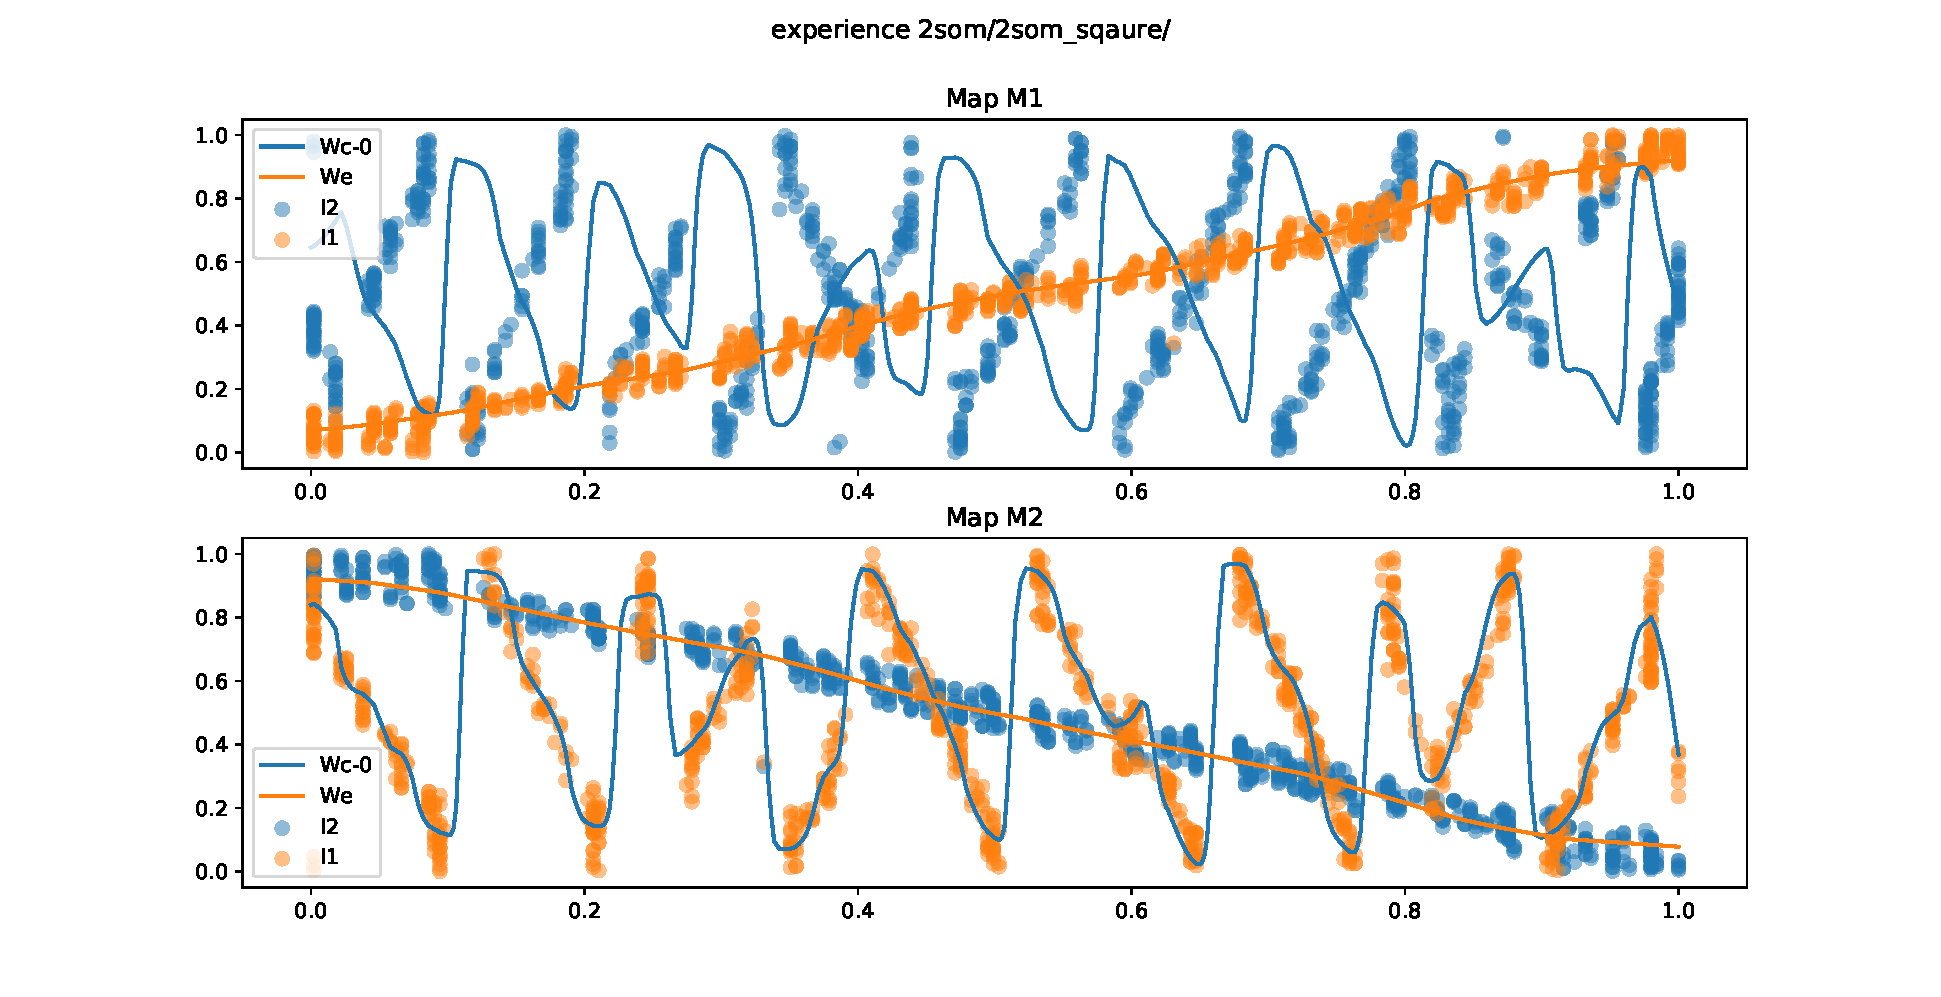
\includegraphics[width=0.7\textwidth]{2som_square_w.pdf}
\end{figure}





\subsection{Conclusion}

Ces architectures de quelques cartes sont des architectures \emph{élémentaires}: toute architecture comportant plus de cartes pourra être construite à partir de petits modules. Nous considérerons les comportements observés dans ce chapitre comme des comportements élémentaires des architectures de cartes.


\section{Analyse de la relaxation}

Le processus de relaxation utilisé dans l'algorithme CxSOM est une méthode originale pour construire des connexions bidirectionnelles entre cartes. Deux cartes connectées de cette façon jouent alors un rôle symétrique, contrairement à une connexion unidirectionnelle ou hiérarchique dans laquelle une carte joue le rôle d'entrée et une autre de sortie. Dans cette section, nous évaluons expérimentalement la méthode de relaxation en tant que moyen de trouver une best matching unit (BMU). 

La Best Matching Unit d'une carte de Kohonen correspond à la position où l'activité est maximale. Dans la situation d'une architecture de plusieurs cartes, ayant chacune un BMU, le vecteur de BMUs correspond à la positions ou chacune des activités est maximale. On est donc face à un problème d'optimisation multi-objectif dans lequel on cherche un seul point maximisant chacune des activités, mais dans lequel les activités dépendent les unes des autres. La relaxation est proposée comme heuristique pour trouver ce point, s'il existe. On cherchera donc à répondre aux questions suivantes:
\begin{itemize}
\item Est-ce que la méthode de relaxation converge ?
\item Est-ce que que cette méthode permet de définir un unique BMU ?
\item Quels sont les paramètres à prendre en compte dans l'algorithme de relaxation ?
\end{itemize}

\subsection{Etude de la convergence des BMUs lors de la relaxation}\label{sec:conv}

\subsubsection{Méthode}

La méthode de relaxation cherche un point de convergence des BMU $\bmu\m{i}$ de l'archchitecture. Nous avons réalisé 1000 itérations de test, à poids figés, à différents temps d'apprentissage, et comptons le nombre de pas nécessaires à la convergence de la relaxation. L'algorithme utilisé pour la relaxation s'arrête automatiquement si la relaxation dépasse $\tau_{max}= 1000$ itérations; on considérera que la relaxation n'a pas atteint un point de convergence si la relaxation atteint ces $\tau_{max}$ itérations.
Pour cette expérience, les entrées sont des points pris sur un cercle en deux dimensions. $\inpx\m{1}$ est l'abscisse d'un point, $\inpx\m{2}$ l'ordonnée.
Théoriquement, plusieurs situations se traduisent par une non-convergence de la relaxation:
\begin{itemize}
\item La relaxation évolue vers un point de convergence, mais trop lentement pour y arriver en moins de 1000 itérations
\item La relaxation évolue vers un cycle limite composé d'un nombre limité d'unités étant alternativement best matching units
\item La relaxation évolue sans répétition de motifs dans la carte : évolution chaotique.
\end{itemize}
Le premier cas est évité car la limite de 1000 itérations est assez grande par rapport à la taille de la carte, les cartes étant de taille 500. Le pas d'évolution de la relaxation est d'une dizaine d'unités. La convergence, si elle existe, est donc rapide. Les cas de non-convergence concernent alors la deuxième et la troisième situation.
Nous observerons plus précisément les trajectoires dans la section suivante; on s'intéresse ici seulement à la question de la convergence.
L'étude de la convergence sera réalisée dans des architectures de 2 et 3 cartes, pour des cartes une dimension et deux dimensions.

\subsubsection{Résultats}
La figure \ref{fig:conv_evolution} présente l'évolution du taux de convergence au cours de l'apprentissage d'une architecture de 2 cartes et 3 cartes. La figure \ref{fig:conv_evolution2D} trace  cette évolution dans le cas de cartes 2D. Pour tracer cette évolution, on effectue des étapes de tests à intervalles réguliers au cours de l'apprentissage, pendant lesquelles les poids ne sont pas mis à jour. Ces tests sont réalisés sur 1000 entrées externes $\inpx\m{1} = X, \inpx\m{2}=Y$ (et $\inpx\m{3}=Z$ pour trois cartes), prises aléatoirement dans l'espace d'entrée. On compte, pour chaque échantillon de test, le nombre de pas nécessaire à la relaxation. Si ce nombre est égal à $\tau_{max}$, on considère que la relaxation n'a pas convergé. On trace alors, en haut, le pourcentage d'échantillons de test pour lesquel la relaxation converge. En bas, on trace le nombre moyen de pas de relaxation nécessaires à la convergence.
Dans chaque cas, on répètera 10 fois l'apprentissage complet et les tests, sur le même espace d'entrée mais des éléments différents. Les tracés des figures \ref{fig:conv_evolution} et \ref{fig:conv_evolution2D} sont la moyenne et l'écart type des valeurs obtenues sur ces 10 répétitions.

Au début de l'apprentissage, lorsque les poids sont initialisés aléatoirement, la relaxation atteint rarement un point de convergence. Lorsque les cartes se déplient, la relaxation évolue vers un point de convergence dans plus de $90 \%$ des cas. Cette évolution est similaire pour des architecture de deux et trois cartes. Les expériences avec des cartes en deux dimensions présentent la même évolution. Le taux de convergence en fin d'apprentissage est plutot situé entre $80 \%$ et $90 \%$.
 
\begin{figure}
\centering
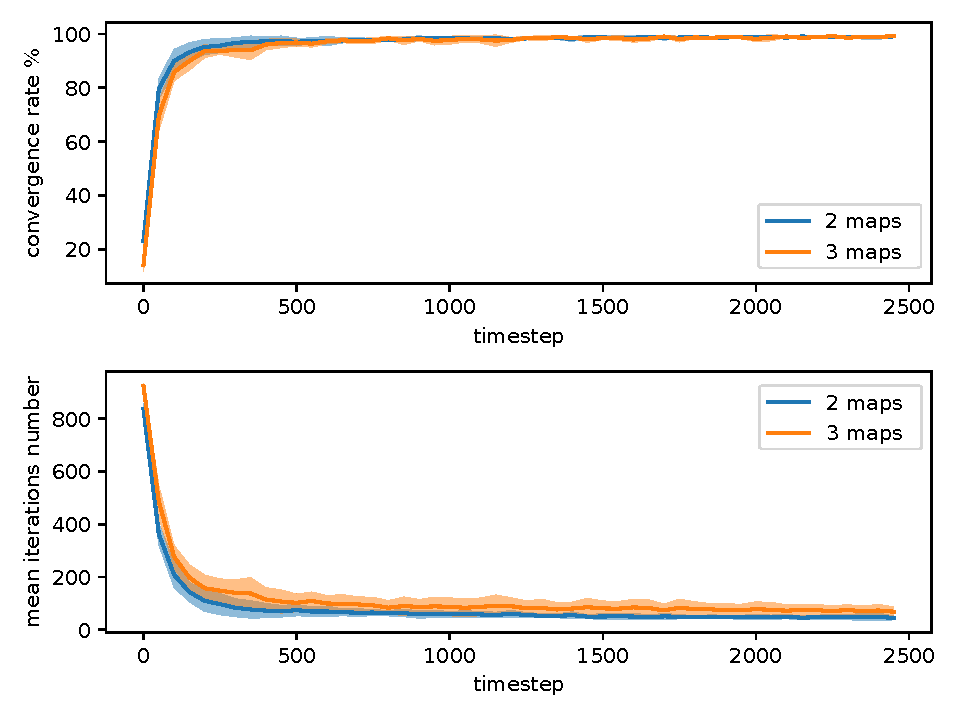
\includegraphics[width=0.7\textwidth]{1D_conv_evolution_total.pdf}
\caption{En haut: évolution de la moyenne et l'écart-type du taux de convergence lors de la relaxation au cours de l'apprentissage sur deux et trois cartes 1D. En bas: évolution du nombre moyen de pas nécessaires à la convergence de la relaxation.
Chaque point est calculé sur un échantillon de 1000 relaxations au temps t, évaluées sur des entrées différentes prises aléatoirement sur le cercle. La moyenne et l'écart-type sont réalisés sur 10 apprentissages séparés.}
\label{fig:conv_evolution}
\end{figure}


\begin{figure}
\centering
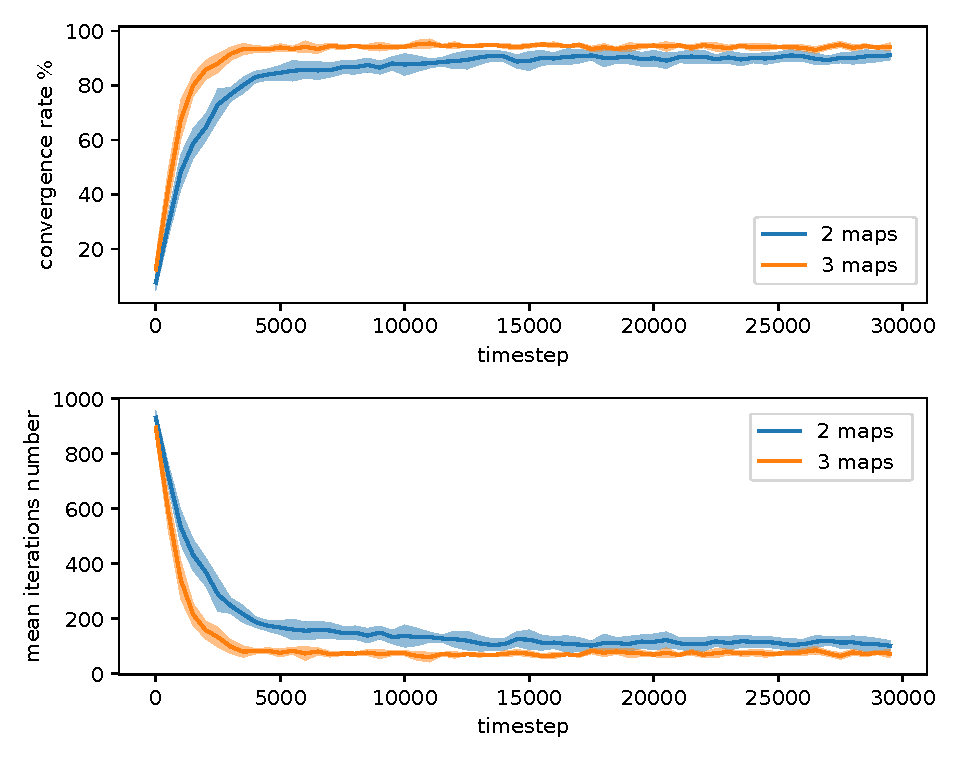
\includegraphics[width=0.7\textwidth]{2D_conv_evolution_total.pdf}
\caption{En haut: évolution de la moyenne et écart type taux de convergence lors de la relaxation au cours de l'apprentissage sur deux et trois cartes 2D. Chaque point est calculé sur un échantillon de 1000 relaxations au temps t, évaluées sur des entrées différentes prises aléatoirement sur le cercle. Les moyennes et écart types sont calculés sur 10 apprentissages séparés.}
\label{fig:conv_evolution2D}
\end{figure}

\subsection{Formalisation de l'algorithme de relaxation}

La relaxation cherche à maximiser de façon \emph{commune} de l'activité globale de chaque carte de l'architecture. Notons $(\mathbf{\bmu})_\tau = (\bmu\m{0}_\tau,\cdots,\bmu\m{N}_\tau)$ la suite définie par l'évolution des BMUs des $N$ cartes d'une architecture lors de la relaxation.
La suite $(\mathbf{\bmu})_\tau$ est une suite définie par récurrence par $\mathbf{\bmu}_{\tau+1} = \mathbf{f}(\mathbf{\bmu}_\tau)$
avec $\mathbf{f} = (f\m{0},\cdots,f\m{N}) : [0,1]^N \rightarrow [0,1]^N$ une application non linéaire transformant l'espace des positions des BMUs; $\mathbf{f}$ ne dépend pas de $\tau$. L'algorithme de relaxation est alors une recherche de point fixe de la fonction $\mathbf{f}$.
Détaillons l'évolution de cette suite. Pour clarifier les notations, définissons pour chaque carte~$i$ $p\star\m{i}_\tau$, comme la position maximisant l'activité globale de la carte $i$:
\begin{equation}
\begin{gathered}
p\star\m{i}_{\tau} = \argmax_{p\m{i}}(a_g\m{i}(p\m{i},\bmu\m{i_0}_\tau, \cdots \bmu\m{i_K}_\tau))\\
 i_0, \cdots i_K \: \text{indices des cartes nourrissant la carte $i$}.
\end{gathered}
\label{eq:pstar}
\end{equation}
$a_g\m{i}$ est une fonction des poids de la carte $\w\ext\m{i}, \w\cont\m{i}$ et de son entrée externe $\inpx\m{i}$. Lors du processus de relaxation, les poids et l'entrée restent fixes. Le calcul de $a_g$ ne dépend pas de $\tau$. Pour toute carte $i$, $p\star\m{i}_{\tau}$ est donc seulement une fonction de $(\bmu\m{i_0}_\tau, \cdots \bmu\m{i_K}_\tau)$.
L'équation d'évolution s'écrit alors: 
\begin{equation}
\bmu\m{i}_{\tau+1} = 
\begin{cases}
\bmu\m{i}_{\tau} + sgn(p\star\m{i}_{\tau} - \bmu\m{i}_{\tau}) \times \delta \; & \text{si $p\star\m{i}_{\tau} - \bmu\m{i}_{\tau} > \delta$ } \\
p\star\m{i}_{\tau} \; \text{sinon}	
\end{cases}
\label{eq:evolution}
\end{equation}

En posant $f\m{i}$ la partie droite de l'équation \ref{eq:evolution}, on peut donc écrire: 
\begin{equation}
\bmu\m{i}_{\tau +1} = f\m{i}(\bmu\m{0}_\tau,\cdots,\bmu\m{N}_\tau)
\label{eq:fonction}
\end{equation}
Soit, pour l'ensemble des composantes : 
\begin{equation}
\mathbf{\bmu}_{\tau+1} = \mathbf{f}(\mathbf{\bmu}_\tau)
\end{equation}

La relaxation se traduit ainsi par une recherche de point fixe de la suite $(\mathbf{\bmu})_{\tau}$, soit une position $\mathbf{\bmu}$ telle que:
\begin{equation}
\mathbf{\bmu} = \mathbf{f}(\mathbf{\bmu})
\label{eq:suite}
\end{equation}

Si $f$ admet un point fixe, alors ce point fixe est aussi un point fixe pour la suite $(\mathbf{\bmu})_\tau$. Cependant, rien ne garantit que ce point fixe existe, et qu'il sera atteint par la suite. Expérimentalement, il semble que si $\mathbf{f}$ admet un unique point fixe et que les poids $\w$ présentent une continuité, alors $(\mathbf{\bmu})_{\tau}$ converge vers ce point fixe. 

L'évolution de la suite $(\mathbf{\bmu})_{\tau}$ dépend de son initialisation.
L'état initial $(\bmu\m{0}_0, \cdots , \bmu\m{N}_0)$ est défini dans CxSOM par: 
\begin{equation}
\begin{cases}
\bmu\m{0}_0 = \argmax_{p\m{0}} a_e(p\m{0},\inpx\m{0})\\
\cdots \\
\bmu\m{N}_0 = \argmax_{p\m{N}} a_e(p\m{N},\inpx\m{N})\\
\end{cases}
\label{eq:init}
\end{equation}

On montrera qu'il n'existe pas toujours un unique point fixe, notamment lorsque les poids sont aléatoires au début de l'apprentissage, ce qui entraîne alors une non-convergence de la relaxation. Cependant, ces cas de non-convergence n'influencent pas l'apprentissage des cartes en choissant des bons paramètres d'apprentissage. On observera expérimentalement qu'à la fin de l'apprentissage, la disposition des poids permet l'existence d'un unique point fixe, indépendant de l'initialisation des valeurs de $\bmu\m {i}_{\tau}$.

Dans les sections suivantes, nous utiliserons des entrées formant un cercle en une dimension dans un espace en deux ou trois dimensions. Les entrées d'une carte correspondent à la coordonnée des points sur un des axes $X$,$Y$ et $Z$ en trois dimensions.
Les architectures étudiées sont des cartes 1D, et 2D lorsque cela est précisé. Les cartes sont connectées réciproquement, comme indiqué en figure \ref{fig:archis}.
Nous chercherons, sur ce jeu de données, à vérifier si la relaxation converge, et comment les paramètres et l'initialisation de la relaxation influencent les trajectoires et la convergence.
\begin{figure}
\centering
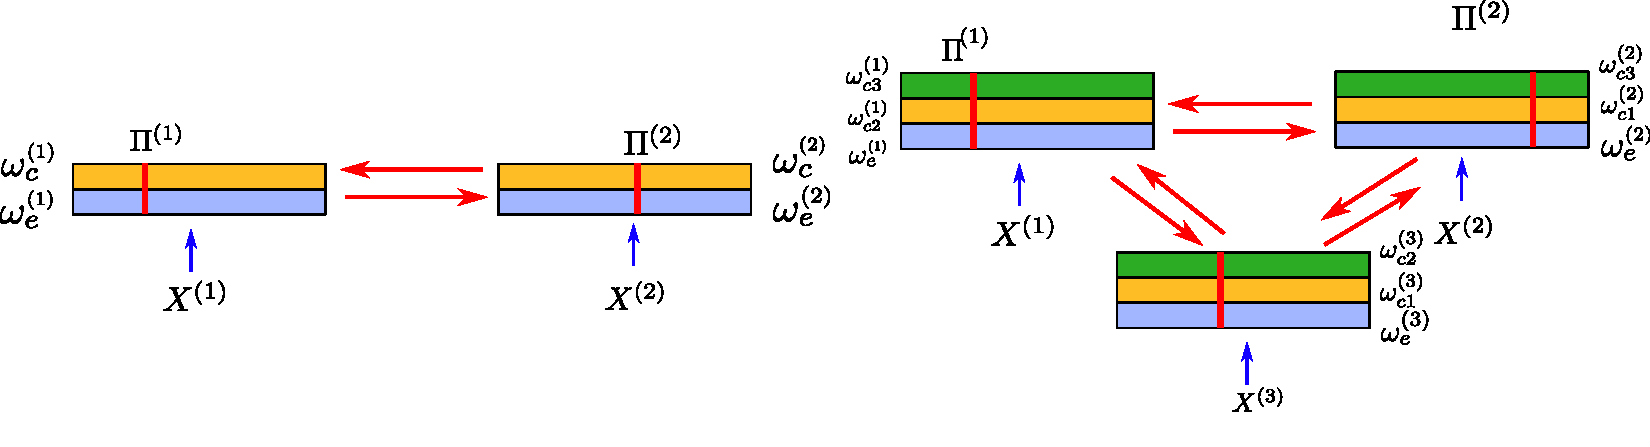
\includegraphics[width=\textwidth]{archis}
\caption{Architectures de deux et trois cartes utilisées dans cette section. Les cartes peuvent être en une ou deux dimensions. Dans le cas de cartes en deux dimensions, la position du BMU $\bmu$ est alors un vecteur 2D.}
\label{fig:archis}
\end{figure}

\subsection{Etude de l'influence de l'entrée contextuelle sur le BMU}\label{sec:cont}

Dans cette section, nous étudions plus précisément l'évolution de la suite $(\mathbf{\bmu})_{\tau}$ dans le cas de d'une architecture de deux cartes 1D connectées. Les cartes sont $M\m{1}$ et $M\m{2}$ prenant en entrée externe respectivement $\inpx\m{1} = X, \inpx\m{2} = Y$, coordonnées des points d'un cercle 2D.
Les entrées contextuelles des deux cartes sont à valeurs dans l'espace des positions d'une carte: $\inpc\m{1} = \bmu\m{2}$ et $\inpc\m{2} = \bmu\m{1}$.
On définit les valeurs $p\star\m{1}$ et $p\star\m{2}$ comme indiqué dans l'équation \ref{eq:pstar}
\begin{equation} 
\begin{cases}
	p\star\m{1}_{\tau} = \argmax_{p\m{1}}(a_g(p\m{1},\bmu\m{2}_{\tau})) \\
	p\star\m{2}_{\tau} = \argmax_{p\m{2}}(a_g(p\m{2},\bmu\m{1}_{\tau})) \\
\end{cases}
\end{equation}

On trace ensuite les valeurs de $p\star\m{1}$ en fonction de son entrée contextuelle $\bmu\m{2} \in [0,1]$, et $p\star\m{2}$ en fonction de $\bmu\m{1} \in [0,1]$ en figure \ref{fig:w006}.
Cette expérience est réalisée après l'apprentissage. On remarque que, $p\star\m{i}$ varie peu en fonction de l'entrée contextuelle de la carte; tout le processus de relaxation se déroulera donc dans une portion réduite de la carte. Cette propriété favorise la convergence de la relaxation.
En réalisant les mêmes tracés à des étapes différentes de l'apprentissage, on remarque que la dépendance de $p\star$ à l'entrée contextuelle dépend surtout de l'organisation des poids externes. En effet, l'activité externe est prépondérante dans le calcul de l'activité globale. Les poids externes s'organisent plus rapidement que les poids contextuels dus à la différence de rayons de voisinage. A partir du moment ou les poids externes d'une carte $i$ sont dépliés, les valeurs possible pour $\bmu\m{i}$ restent dans une portion limitée de la carte. Cela permet alors à la relaxation de trouver un point fixe dans cette portion.

\begin{figure}
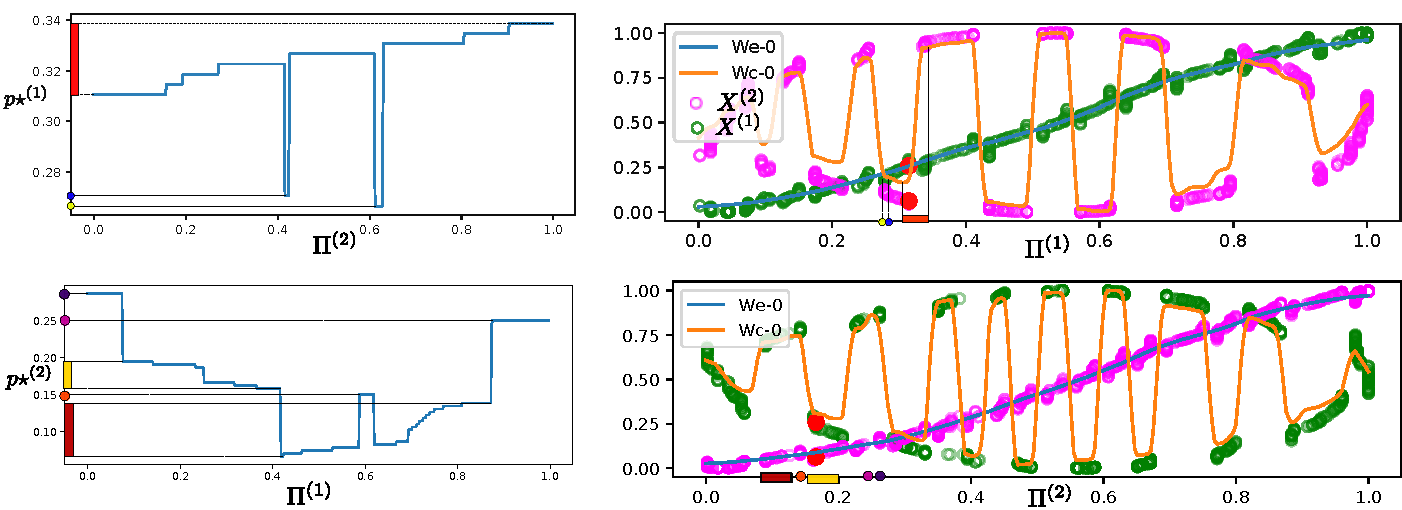
\includegraphics[width=\textwidth]{am_w_006}
\caption{(a): $p\star\m{1}$ et $p\star\m{2}$ en fonction de l'entrée contextuelle de leur carte $\bmu\m{2}$ et $\bmu\m{1}$.(b): les poids externes et contextuels des cartes $1$ et $2$ sont représentés selon leur position dans la carte. On représente également les entrées test $\inpx\m{1}$ et $\inpx\m{2}$ en fonction de leur BMU. Les entrées utilisées pour tracer les figures de gauche sont colorées en rouge sur les figure de droite: $\inpx\m{1}=0.26,\inpx\m{2}=0.06$. Les intervalles dans lequel les valeurs de $p\star$ varient sont reportés sur la figure (b).}
\label{fig:w006}
\end{figure}



\subsection{Etude de l'unicité du point fixe}\label{sec:pf}

Nous étudions dans cette partie l'évolution de processus de relaxation lancés sur les mêmes poids, pour une entrée externe fixée, mais avec $\mathbf{\bmu}_0$ intialisés à des valeurs aléatoires dans chaque carte.
En figure \ref{fig:diff_relax_t1_notraj} et \ref{fig:diff_relax_notraj}, nous représentons les valeurs $\lvert p\star\m{1} - p\m{1} \rvert$ et $\lvert p\star\m{2} - p\m{2}\rvert$ en fonction de $p\m{1},p\m{2} \in [0,1]$, au début et fin de l'apprenitssage. On rappelle que $p\star\m{1}$ dépend de $p\m{2}$, et inversement.
Le point fixe, s'il existe, est alors à une position $p\m{1},p\m{2}$ vérifiant:
\begin{equation*}
\begin{cases}
p\star\m{1} = p\m{1}\\
p\star\m{2} = p\m{2}\\
\end{cases}
\end{equation*}

On effectue 200 trajectoires de relaxation, initialisées à $\bmu\m{1}_0,\bmu\m{2}_0$ différents. Leurs valeurs finales sont représentées par un point noir en figures \ref{fig:diff_relax_t1_notraj} et \ref{fig:diff_relax_notraj}. 
Au début de l'apprentissage, la fonction de relaxation présente plusieurs points d'attraction, représentés par les points noirs en figure \ref{fig:diff_relax_t1_notraj}. Cette non-convergence semble s'expliquer par les valeurs des différences $\lvert p\star\m{1} - p\m{1} \rvert$ et $\lvert p\star\m{2} - p\m{2}\rvert$. Les zones en violet sur chaque figure représentent les positions où ces différences sont nulles, sur la carte 1 et 2. Un point fixe se trouve sur une position telle que les différences sont nulles dans les deux figures. Une telle position semble exister en figure \ref{fig:diff_relax_t1_notraj}, mais peu de trajectoires de relaxation y aboutissent. La figure \ref{fig:champ_0} représente le déplacement à effectuer de $(\bmu\m{1},\bmu\m{2})$ lors de la relaxation en fonction de la position courante. Les trajectoires des relaxations y sont également représentées. Le champ de déplacement ne semble pas permettre de trouver un point de convergence.
A la fin de l'apprentissage, ce qui est représenté en figure \ref{fig:diff_relax_notraj}, un point fixe semble exister. Ce point correspond à la position où les deux différences $\lvert p\star\m{1} - p\m{1} \rvert$ et $\lvert p\star\m{2} - p\m{2}\rvert$ sont nulles. Les 200 trajectoires mènent au même point, il semble donc être un point de convergence commun à toutes les initialisations pour la relaxation. La figure \ref{fig:champ_9999} présente le champ de déplacement des BMUs en fonction de la position courante. Les trajectoires suivent les zones où l'une ou l'autre des différences est nulle, pour mener à la position stable. 

\begin{figure}
\begin{minipage}{0.5\textwidth}
\centering
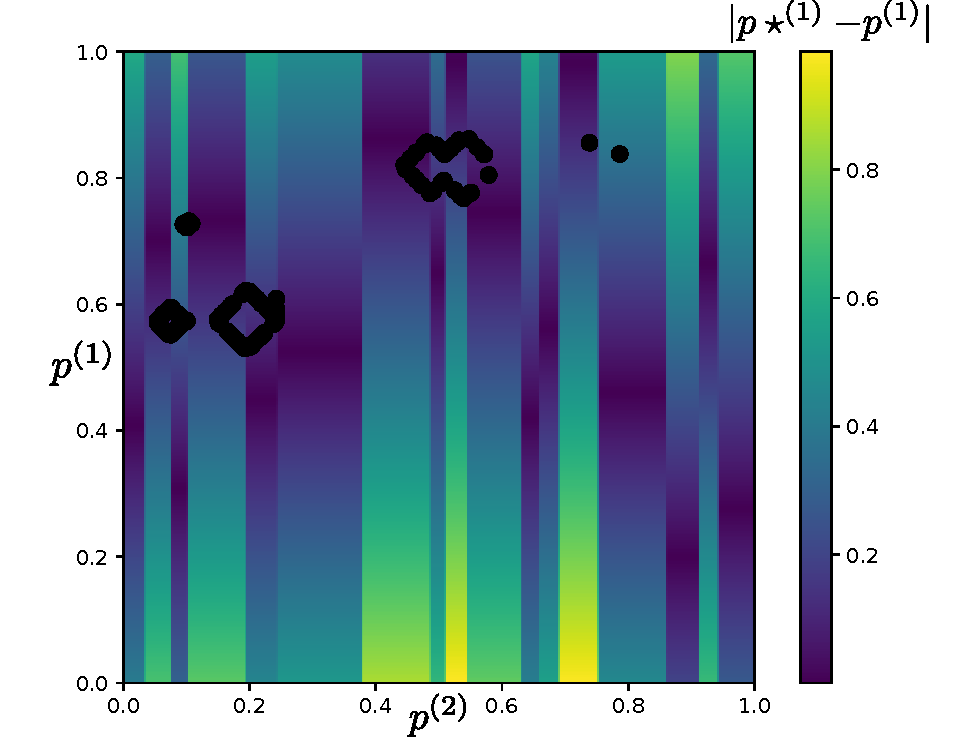
\includegraphics[width=\textwidth]{champ_X_006_t1_notraj.pdf}
\end{minipage}
\begin{minipage}{0.5\textwidth}
\centering
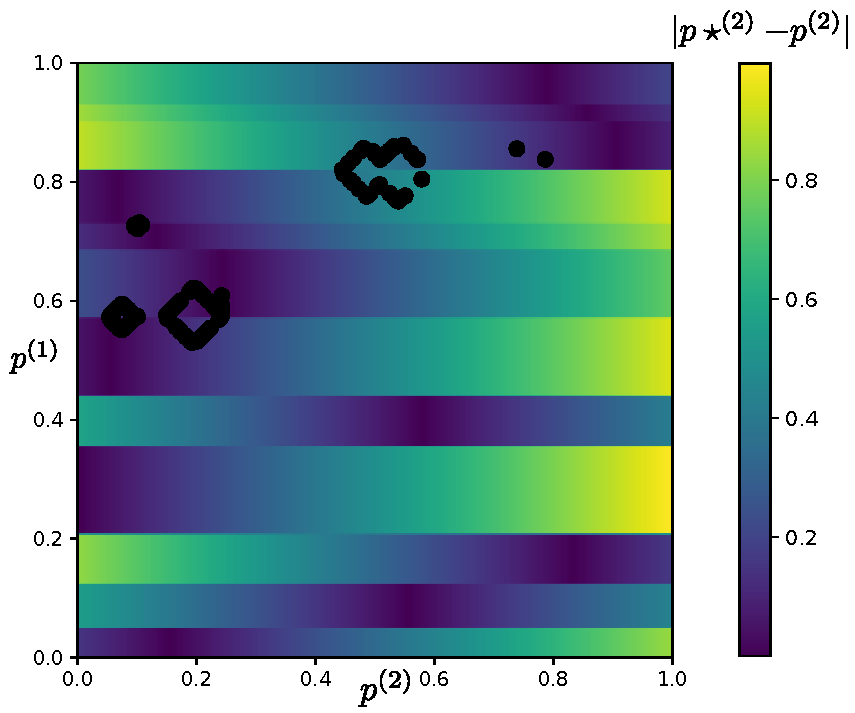
\includegraphics[width=\textwidth]{champ_Y_006_t1_notraj.pdf}
\end{minipage}
\caption{Valeur de ${p\star}\m{1} - p\m{1}$, resp. ${p\star}\m{2} - p\m{2}$ à $t=0$ ,lorsque les poids sont encore aléatoiremement disposés dans chaque carte.
 ${p\star}\m{1}$ ne dépend que de $p\m{2}$ : on peut donc tracer cette valeur selon deux dimensions pour chaque carte. Les zones où cette valeur est nulle sont en violet sur le graphique. Les points fixes, s'il existent, sont aux positions de différence nulle pour $M\m{1}$ et $M\m{2}$. Les points noirs représentent les points de convergence pour 200 trajectoires de relaxation, lancées pour différents $\bmu_0\m{1}, \bmu_0\m{2}$.}
 
\label{fig:diff_relax_t1_notraj}
\end{figure}

\begin{figure}
\begin{minipage}{0.5\textwidth}
\centering
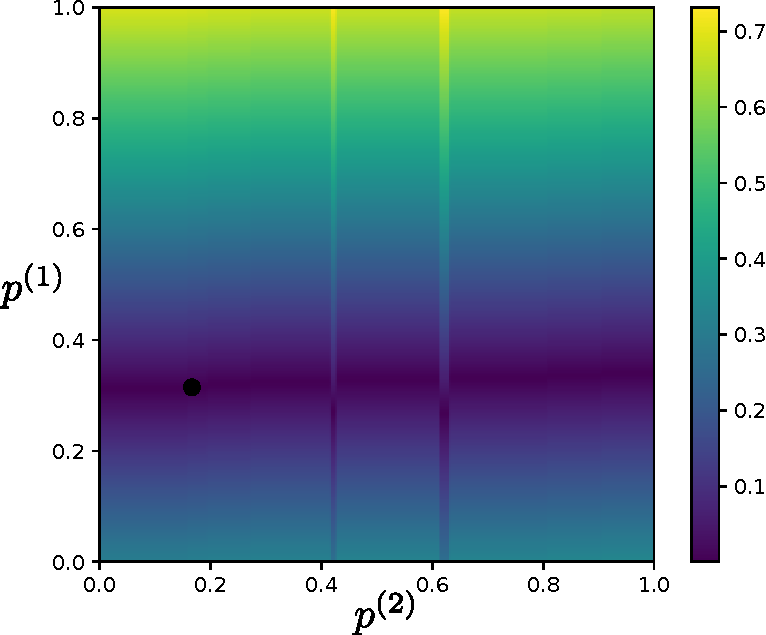
\includegraphics[width=\textwidth]{champ_X_006_notraj.pdf}
\end{minipage}
\begin{minipage}{0.5\textwidth}
\centering
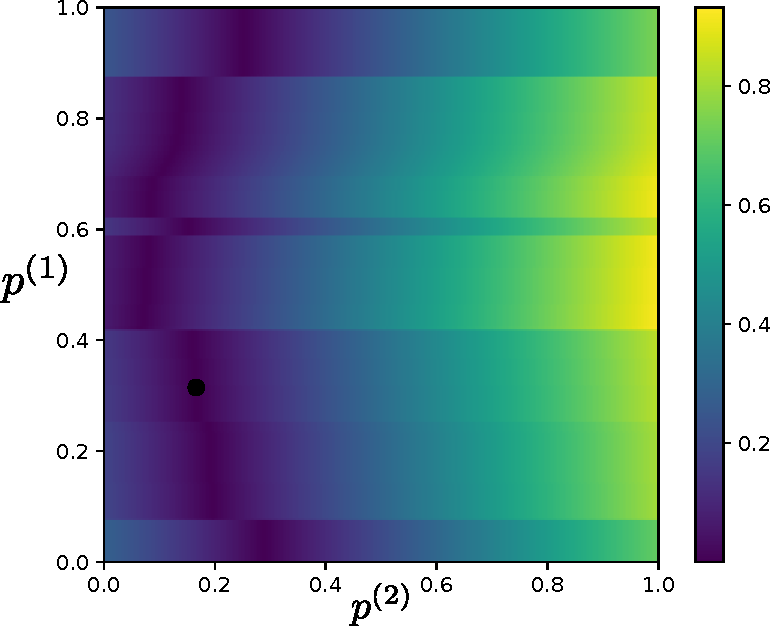
\includegraphics[width=\textwidth]{champ_Y_006_notraj.pdf}
\end{minipage}
\caption{Valeur de ${p\star}\m{1} - p\m{1}$, resp. ${p\star}\m{2} - p\m{2}$, lorsque les cartes sont organisées telles qu'en figure \ref{fig:w006}. ${p\star}\m{1}$ ne dépend que de $p\m{2}$ : on peut donc tracer cette valeur selon deux dimensions pour chaque carte. Les zones où cette valeur est nulle sont en violet sur le graphique. Les points fixes, s'il existent, sont aux positions de différence nulle pour $M\m{1}$ et $M\m{2}$. Les points noirs représentent les points d'arrivée de la relaxation pour 50 trajectoires de relaxation, lancées pour différents $\bmu_0\m{1}, \bmu_0\m{2}$. La relaxation semble présenter un point de convergence, qui se situe sur un point fixe de la fonction de relaxation.}
\label{fig:diff_relax_notraj}
\end{figure}

\begin{figure}
\centering
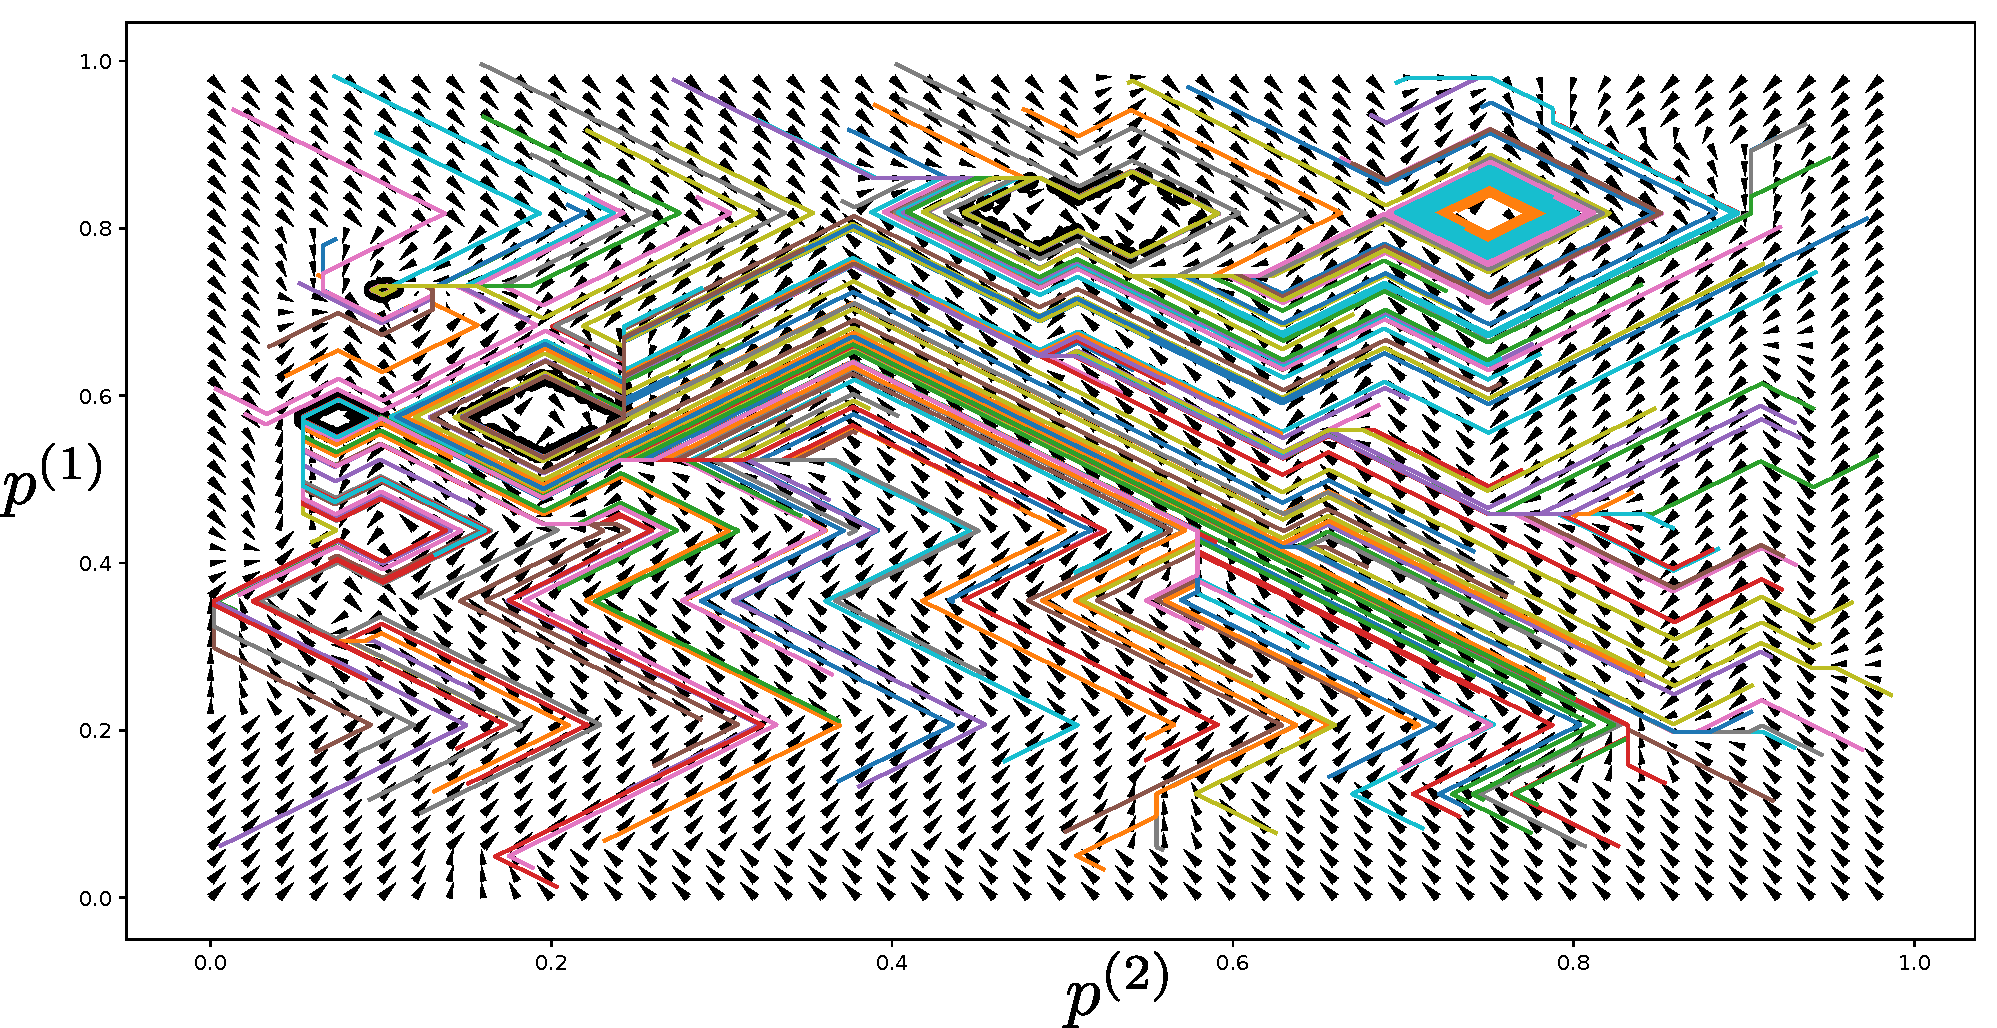
\includegraphics[width=\textwidth]{champ_006_t1.pdf}
\caption{Champ de déplacements de $\bmu\m{1},\bmu\m{2}$ lorsque les poids sont encore aléatoires, à $t=0$. Les trajectoires de 200 relaxations, initialisées différemment, sont représentées. En fonction de la position initiale des BMUs, la relaxation évolue vers un point fixe ou un cycle limite. }
\label{fig:champ_0}
\end{figure}


\begin{figure}
\centering
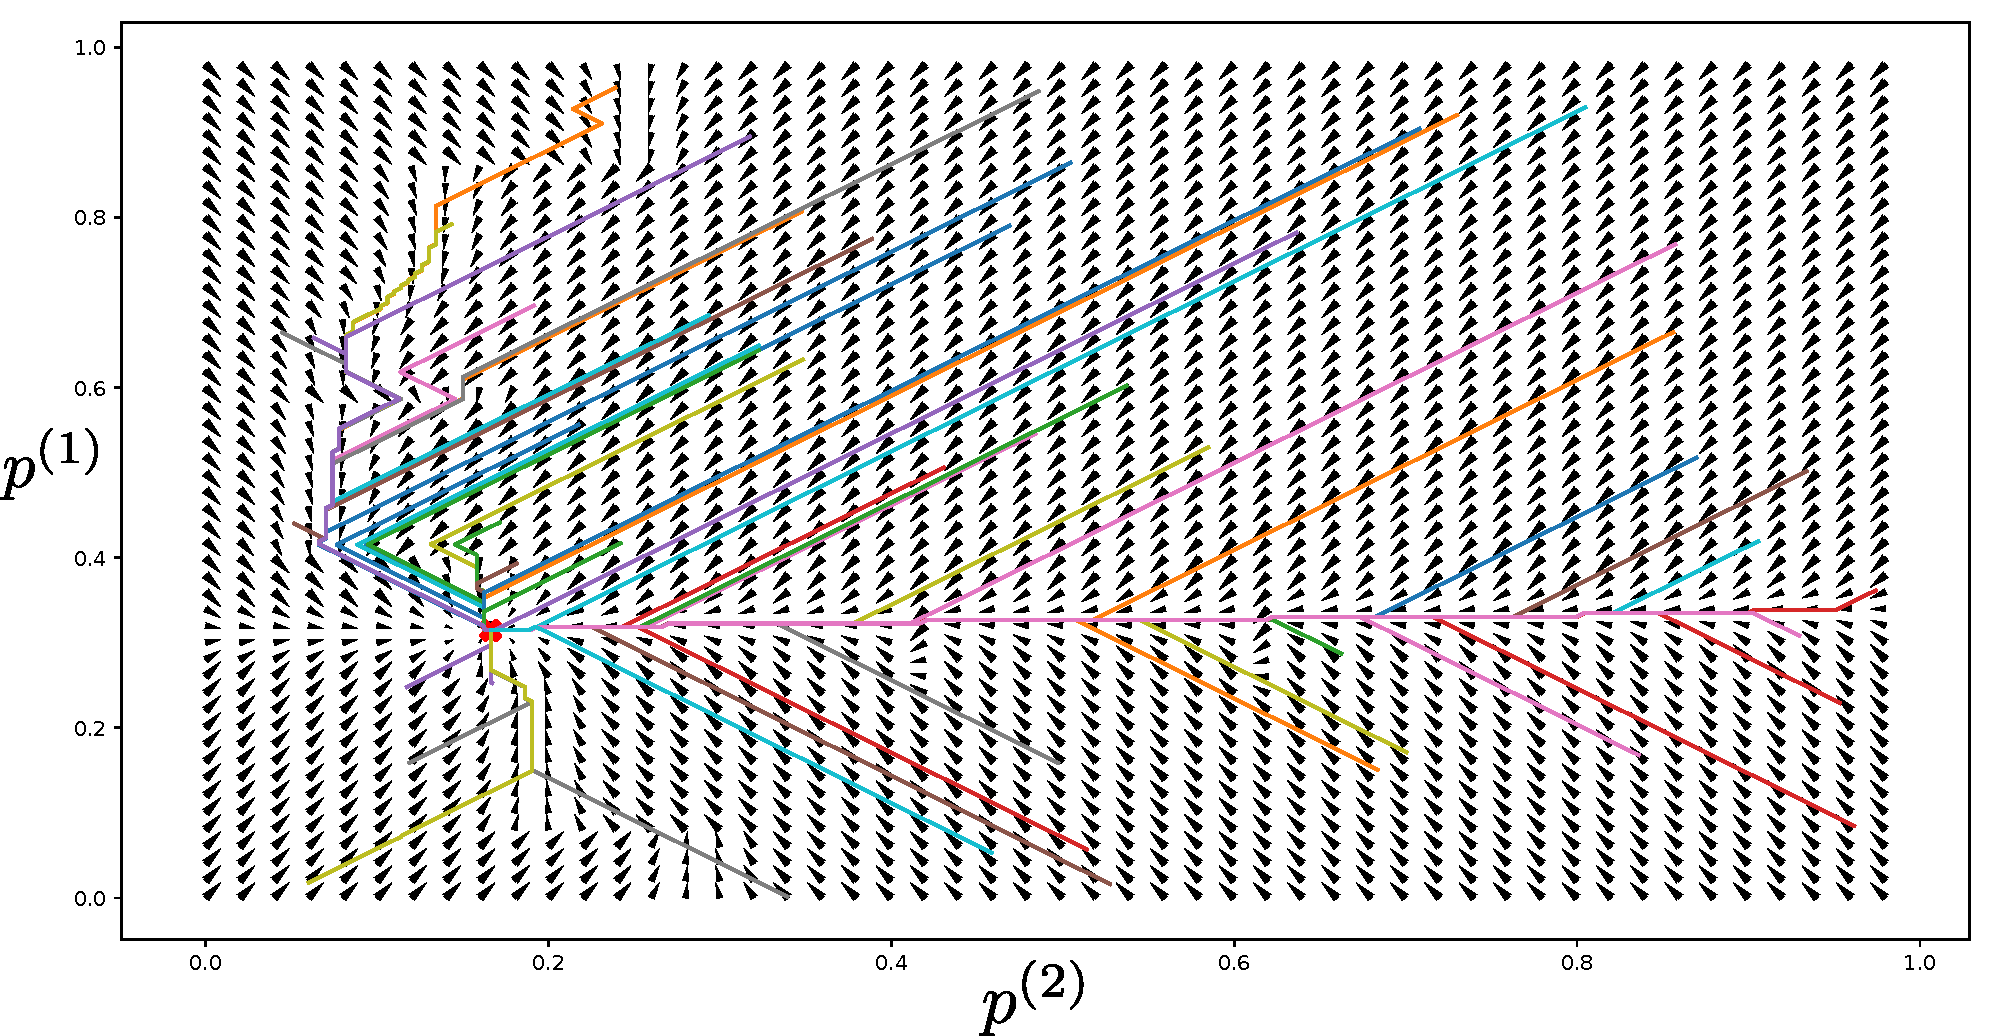
\includegraphics[width=\textwidth]{champ_006.pdf}
\caption{Champ de déplacements de $\bmu\m{1},\bmu\m{2}$ lorsque les poids sont organisés tels que représentés en figure \ref{fig:w006}, à $t=9999$.es trajectoires de 50  relaxations, initialisées différemment, sont représentées. Les relaxations évoluent vers un point fixe commun.}
\label{fig:champ_9999}
\end{figure}

\subsection{Influence du pas de convergence}

Dans les expériences précédentes, on a utilisé un pas de convergence $\delta=0.05$. Une autre solution est de ne pas utiliser de pas de relaxation, c'est à dire, à chaque itération, déplacer le BMU $\bmu\m{i}$ directement à la position ou l'activité globale est maximale, au lieu de le déplacer de $\delta$ vers cette position.
L'évolution de la relaxation devient alors:
\begin{equation}
\forall i, \bmu\m{i}_{\tau+1} = p\star\m{i}_{\tau}
\end{equation}
En figure \ref{fig:diff_nopas}, on trace différentes trajectoires de relaxation, pour une même entrée. Ces relaxation sont effectués après l'apprentissage des données par l'architecture. Le processus de relaxation effectué pendant l'apprentissage n'utilise pas de déplacement $\delta$ non plus. 
On représente sur cette même figure les différences ${p\star}\m{1} - p\m{1}$ et ${p\star}\m{2} - p\m{2}$. La relaxation semble encore converger vers un point fixe.


\begin{figure}
\begin{minipage}{0.5\textwidth}
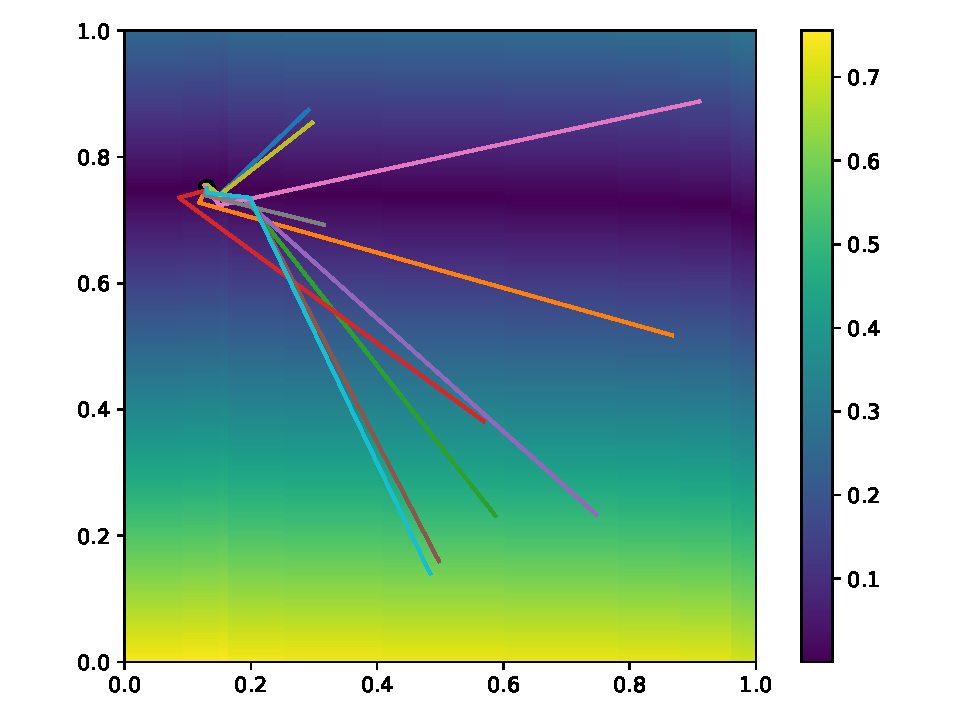
\includegraphics[width=\textwidth]{champ_X_009}
\end{minipage}
\begin{minipage}{0.5\textwidth}
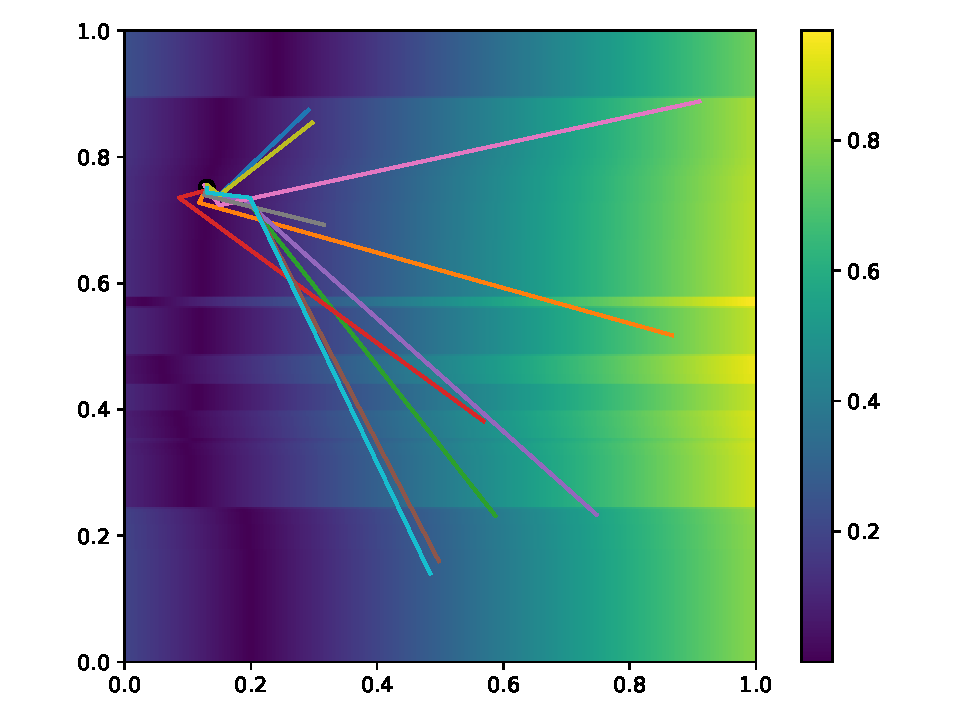
\includegraphics[width=\textwidth]{champ_Y_009}
\end{minipage}
\caption{Trajectoires des relaxations $(\bmu\m{1}_{\tau},\bmu\m{2}_\tau)$ dans le champ des différences ${p\star}\m{1} - p\m{1}$ et ${p\star}\m{2} - p\m{2}$, lorsque la relaxation est effectuée sans utiliser de petits déplacements. Les tracés sont effectués après apprentissage. La relaxation semble encore converger vers un point fixe.}
\label{fig:diff_nopas}
\end{figure}

\subsection{Discussion}
Les parties \ref{sec:conv} et \ref{sec:cont} montrent que, lorsque les poids sont quelconques, la convergence de l'algorithme de relaxation n'est pas assurée; au contraire, la relaxation évolue dans la plupart des cas vers une situation non convergente. Dans le cas particulier étudié dans la section, il semble exister des point fixes, mais dus au caractère aléatoire des poids. La relaxation ne permet pas de trouver ces points. Pourtant, l'apprentissage des cartes utilisant la relaxation comme recherche de BMU mène une organisation des poids, même sans que la relaxation ne converge au début. Cette organisation permet de plus une meilleure convergence de la relaxation (convergence dans plus de $90 \%$ des cas).

Ce comportement peut être expliqué. On observe que la relaxation converge bien à partir du moment où les poids externes sont organisés et présentent une continuité. Au début de l'apprentissage, même si la relaxation mène à des positions quelconques de BMUs, ces BMUs auront quand même des poids externes proches de la valeur de l'entrée. Le calcul de l'activité dépend en effet d'abord de l'activité externe de la carte:
$$ a_g = \sqrt{a_e ( \beta a_e + (1-\beta a_c))}, \;\; \beta=0.5$$ 
De plus, la relaxation est initialisée à une position correspondant au maximum de l'activité externe.
L'organisation de la carte s'effectuera donc de façon similaire à une carte classique. Dans une carte de Kohonen, pour des poids aléatoires, de multiples positions de BMU sont possibles lors du calcul de la distance des poids à l'entrée. La disposition des poids et le choix du BMU n'influencent pas la propriété globale d'organisation d'une carte. Cette même observation peut s'effectuer ici. 
Le rayon de voisinage externe étant bien plus grand que le rayon de voisinage contextuel, l'organisation des poids externes de la carte influence peu l'organisation des poids contextuels.
Lorsque les poids externes présentent une continuité, la relaxation converge. Les poids contextuels peuvent alors s'organiser selon le BMU, qui a maintenant un sens: il s'agit d'un point fixe de la fonction de relaxation. Le BMU correspond alors au point qui maximise en même temps les activités globale de chaque carte.

Expérimentalement, on observe que, lorsque les cartes sont organisés, le point fixe est atteint par n'importe quelle trajectoire de relaxation. Le BMU a donc un sens au niveau de la carte. 

Enfin, la relaxation dépend du pas de déplacement utilisé $\delta$. On pourrait supposer que prendre un petit $\delta$ permet une meilleure convergence; en fait, la valeur de $\delta$ influence peu la capacité de convergence et l'organisation des cartes. La relaxation pourrait être effectuée sans utiliser de pas de relaxation. Par ailleurs, la relaxation est initialisée proche de la position théorique du BMU, quand elle existe. La relaxation est donc finalement assez courte.

\subsection{Conclusion}
La relaxation est donc une recherche d'un maximum global à l'architecture, ce maximum étant un point fixe de la fonction de mise à jour des positions.
Une fois que les poids externes d'une carte présentent une continuité, la relaxation et le BMU issu de ce processus ont un sens topologique: on observe expérimentalement que la fonction de mise à jour présente un point fixe $\mathbf{\bmu} = \mathbf{f}(\mathbf{\bmu})$, et que la relaxation converge vers ce point fixe. Ce point fixe est alors le point qui maximise \emph{collectivement} les activités globales de chaque carte de l'architecture.
Bien que la relaxation ne converge pas au début de l'apprentissage, la convergence est observée dès que les poids externes présentent une certaine continuité. Cette continuité étant assurée après quelques itérations d'apprentissage par l'algorithme de mise à jours des poids de Kohonen, on peut donc dire que la relaxation converge au sein de CxSOM. Cette convergence est observée pour des cartes en une et deux dimensions.
La relaxation est alors un moyen de trouver un ensemble de BMU au sein d'une architecture maximisant une propriété \emph{globale} à cette architecture: toutes les cartes voient leur activité globale maximisée. Les BMUs ont donc un sens topologique. Cette recherche de maximum est réalisée localement, au niveau de chaque carte, et non de façon globale. La relaxation agit alors comme une manière de connecter des cartes de façon non-hiérarchique, avec un calcul décentralisé.



\chapter{Application: prédiction d'entrée manquante}
\graphicspath{{05-Application/}}
\minitoc

Dans ce chapitre final, nous proposons une série d'expériences autour de tâches de prédiction de modalité par des structures de cartes CxSOM.
Nous nous placons dans un cadre d'application de mémoire associative.

L'une des motivations de la construction d'une architecture de cartes de Kohonen est de constuire des systèmes de cartes autonomes, notamment en robotique; c'est à dire, un système de carte capable d'effectuer de la prise de décision à partir des calculs effectués dans chaque carte, à savoir le calcul de BMU.
Dans un contexte de mémoire associative, cette prise de décision se rapporte à la prédiction d'une modalité à partir des autres modalités. Ces modalités étant dépendantes les unes des autres, nous attendons de cette prédiciton d'être en accord avec les autres entrées présentées à l'architecture.

Nous avons étudié comment des architectures CxSOM apprennent une représentation interne des relations entre modalités.
La capacité d'une architecture à prédire une modalité traduit l'existence de cette représentation interne.
Dans une architecture CxSOM, une carte ne recevant pas d'entrée externe possède une activité générée par ses entrées contextuelles.
Après apprentissage sur toutes les modalités, toutes les cartes ont des poids externes et contextuels dépliés.
Grâce aux entrées contextuelles, la présentation d'une entrée externe à seulement l'une des cartes permet à chaque carte de l'architecture d'avoir une activité et donc un BMU. Le poids externe de ce BMU peut alors être interprété comme une prédiction de la modalité correspondante.
Nous utiliserons cette propriété dans ce chapitre pour prédire la modalité relative à une carte. La qualité de cette prédiction témoignera de l'apprentissage d'une représentation interne cohérente par l'architecture de cartes. 
Ce chapitre propose une première application de CxSOM dans un cadre de prédiction d'entrée manquante. Nous étudierons comment cette prédiction est mise en oeuvre par l'architecture de cartes. Nous étudierons cette prédiction dans le cadre d'entrées géométriques, puis l'appliquerons à de la prise de décision pour la commande d'un drône.

\section{Prédiction d'entrées géométriques}

Avant d'effectuer des tâches de prédiction dans un cadre réel, nous réalisons des expériences sur les modèles d'entrées géométriques étudiés tout au long de la thèse
Nous étudierons ainsi la prédiction d'une modalité dans le cadre du cercle en 3D et de la sphère 3D. 
Nous prenons dans cette section des architectures de trois cartes connectées de façon rétroactive. 
Le but de 

\subsection{Algorithme de prédiction}

L'étape de prédiction est effectuée après apprentissage sur toutes les modalités.
Lors de la phase d'apprentissage, chaque carte de l'architecture possède une entrée externe. Après l'apprentissage, les poids sont figés.
Pour prédire une modalité $i$, les entrées externes de la carte ayant appris cette modalité ne lui sont plus présentées. Les autres cartes prennent quant à elles une entrée externe.
La carte ayant été "fermée" fait alors office de module de prédiction. Son activité est guidée par ses entrées contextuelles: l'activité globale est alors prise comme la moyenne des activités contextuelles. Le processus de relaxation est réalisé pour chaque entrée présentée à l'architetcture.
La carte correspondant à la modalité à prédire possède une couche de poids externes préalablement organisée lors de la phase d'apprentissage. Le poids externe du BMU, $\w\ext\m{i}(\bmu\m{i})$ est alors utilisé comme prédiction de la modalité manquante. 
Notons que la prédiction d'entrée par l'architecture CxSOM se passe d'utiliser un algorithme supplémentaire. Elle résulte de la dynamique du système de cartes. De cette façon, nous nous rapprochons de l'idée d'un système de carte autonome.

\begin{figure}
\centering
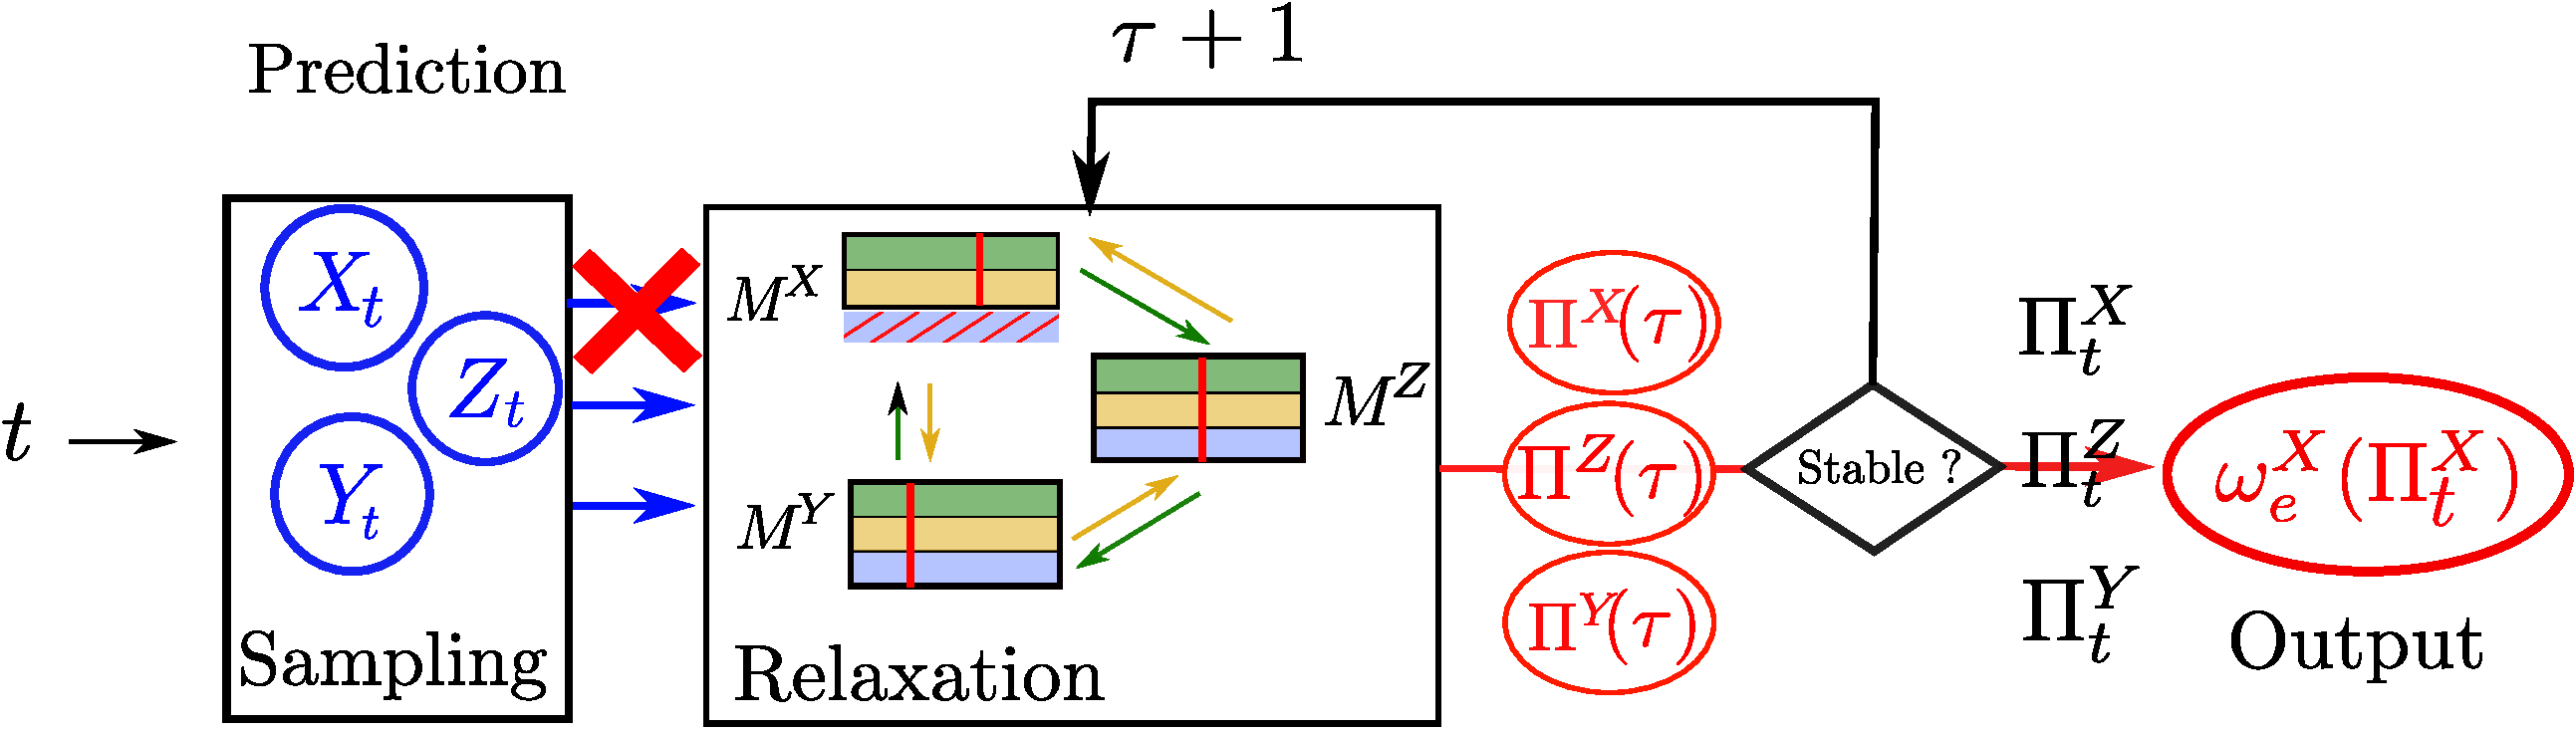
\includegraphics[width=\textwidth]{prediction_setup}
\caption{Description de l'algorithme de prédiction. Il s'agit du même algorithme que pour les tests, sans apprentissage, mais une modalité n'est pas présentée à l'architecture. Le poids externe du BMU de la carte correspondant à la modalité manquante est utilisé comme la prédiction de cette modalité.}
\label{fig:schema}
\end{figure}


\subsection{Résultats}
La figure \ref{fig:pred} représente la valeur de la prédicton $\w\ext\m{1}(\bmu\m{1})$ en fonction de la valeur théorique de cette entrée. 
\begin{figure}
\centering
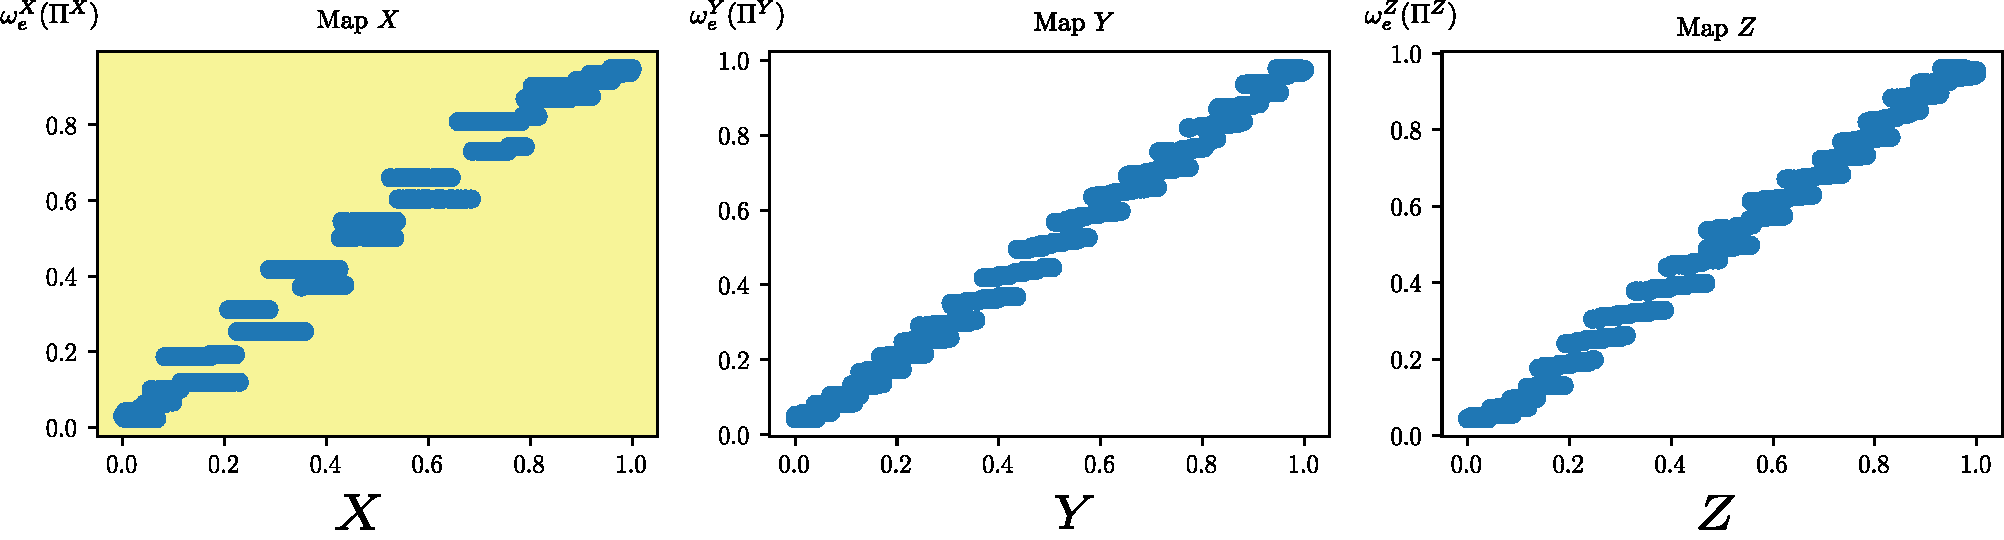
\includegraphics[width=\textwidth]{prediction_x2}
\caption{Prediction de x}
\label{fig:pred}
\end{figure}


\subsection{Discussion}
Les résultats sur des entrées géométriques montrent une bonne capacité de prédiction d'entrée.
La précision est limitée, mais on peut voir cette capacité de prédiction plus comme une preuve de mémoire associative que d'application pratique.
Ce qu'on cherche par la mémoire associative, c'est d'abord d'évoquer une modalité à partir d'autres. Ici, grâce à la connexion entre carte, on génère une zone de valeur limitée pour la modalité $X$: une région est activée, qui est reliée aux valeurs de $X$.
On va plutot parler d'évocation plutot que de prédiction. 

\section{Application à la commande de drône en vol}

Nous sortons du cadre des entrées simulées pour nous placer dans un cas de contrôle réel. Nous disposons d'un drône quadricoptère, commandé à distance. Ce drône possède une caméra frontale ainsi qu'un ensemble de capteurs internes. Chacun de ces capteurs peut être considéré comme une modalité d'un espace multimodal. A ces modalités s'ajoute la modalité correspondant à la commande envoyée au drône.
Le principe est d'apprendre, à l'aide d'une architecture de cartes, les relations existants entre les modalités des capteurs et de la commande afin d'ensuite prédire la commande à envoyer à partir des capteurs.
Afin que les relations entre la commande et les capteurs soient significatives, nous nous placons dans un cas d'application particulier: le drône vole dans un couloir étroit, en ligne droite. Le but du drône est alors de voler en avant dans le couloir, sans toucher les murs.
Le but de cette expérience est de démontrer la tâche de prédiction en situation réelle. Nous évaluerons ainsi la robustesse de l'algorithme à des données bruitées, et la capacité de CxSOM à réagir en temps réel malgré la relaxation.

\subsection{Méthode expérimentale}

Le drône utilisé pour l'expérience est un quadricoptère. Il possède une caméra frontale.
Le drône est contrôlé à distance par un ordinateur; la commande est réalisée en envoyant l'accélération angulaire du drône autour de ses trois axes de rotation.
Nous avons accès aux données des capteurs internes, notamment la vitesse linéaire courante selon chaque axe de déplacement.

le drône se déplace dans un couloir étroit.
Dans le cadre de l'expérience, nous extrayons deux éléments visuels spécifiques au couloir à partir de la caméra du drône: l'abscisse du point de fuite du couloir $x$. Nous calculons également la différence entre les angles du couloir, notée $\varphi$. Ces valeurs sont illustrées en figure~\ref{fig:drone}.
Le drône se déplace dans un couloir, à hauteur constante et vitesse constante.
La commande générant le déplacement en avant du drône (tangage) est maintenue constante. Les commandes permettant le déplacement en largeur sont alors $\omega$ et $\rho$. Dans le cadre de cette expérience, nous contrôlerons uniquement $\rho$.
Enfin, la vitesse linéaire en largeur du drône peut être récupérée à chaque instant; nous la notons $v$.
Nous avons ainsi quatres modalités lors du déplacement du drône: $x$, $\varphi$, $\rho$ et $v$.
Nous construisons une architecture CxSOM sur ces quatres modalités, composée de quatre cartes connectées chacune aux trois autres.
Une phase d'apprentissage est réalisée sur des déplacements du drône contrôlés humainement. Notons que lors de cette phase, nous avons utilisé un système de contrôle PID pour assister la commande humaine. Cette phase d'apprentissage est réalisée hors ligne pour que les données soient réparties aléatoirement.
Après apprentissage, nous effectuons une phase de prédiction. Lors de cette étape, la commande $\rho$ n'est plus présentée à la carte correspondante. Nous envoyons alors le poids externe du BMU de cette carte comme commande du drône. Cette étape est réalisée en ligne, sur des trajectoires réelles du drône.

La figure \ref{fig:drone_inp} présente la répartition des entrées présentées au drône. Nous avons tracé les dépendances entre chaque modalité. Nous remarquons sur la figure qu'une dépendance forte se dégage entre les entrées ?? et ??, ainsi que ?? et ??. Si les cartes apprennent correctement le modèle liant les entrées, la prédiction peut être réalisée.
Ces dépendances sont très bruitées. Cette expérience en conditions réelles nous permettra d'observer la résistance au bruit de la prédiction.

%TODO mettre disposition des entrées.

\subsection{Résultats}
La carte associée à $\rho$ possède donc une couche de poids externe et trois couches de poids contextuels. Ces poids sont représentés en figure \ref{fig:drone_w}. L'organisation des poids contextuels rappelle celle observé dans des conditions géométriques: les poids contextuels définissent des zones. Contrairement à l'expérience réalisée sur un cercle, la taille de ces zones dépend de la couche de poids contextuel définie. 

\begin{figure}
\begin{minipage}{0.5\textwidth}
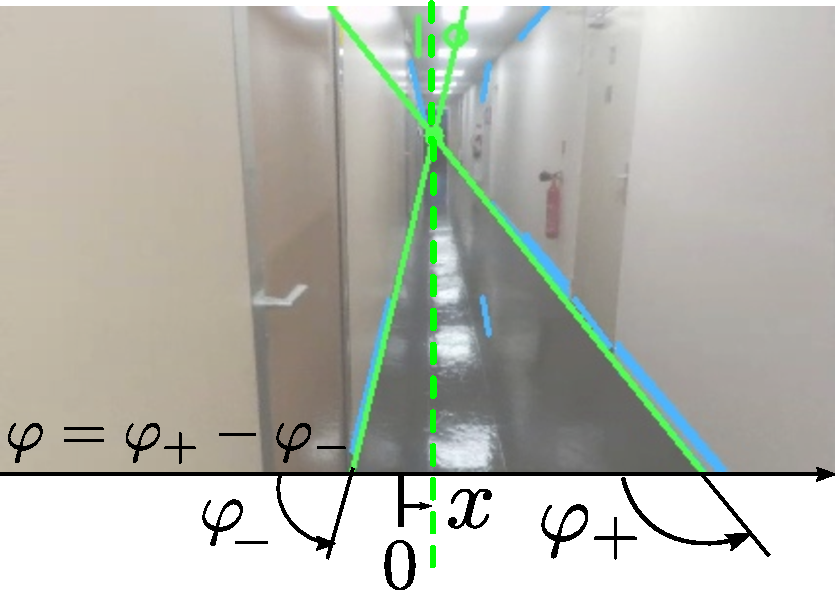
\includegraphics[width=\textwidth]{visudrone}
\end{minipage}
\begin{minipage}{0.5\textwidth}
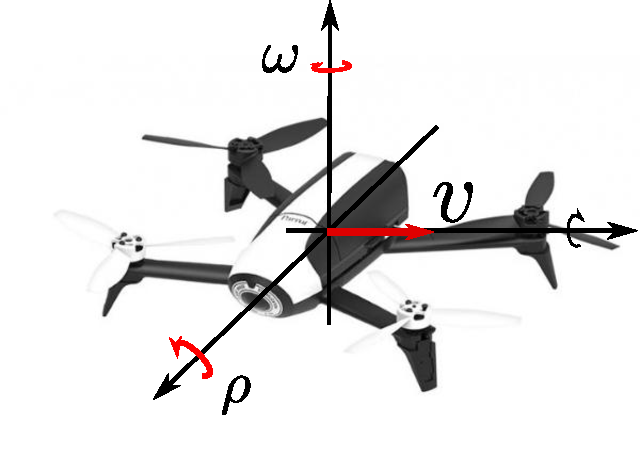
\includegraphics[width=\textwidth]{dronesteup}
\end{minipage}
\caption{Disposition des capteurs utilisés pour l'experience}
\label{fig:drone}
\end{figure}

\begin{figure}
\includegraphics[width=\textwidth]{dronemap}
\caption{Disposition des poids de la carte $\rho$ après apprentissage et exemple de calcul d'activité}
\label{fig:drone_w}
\end{figure}

\subsection{Discussion}
Ici on ne cherchait pas à comparer avec des valeurs théorique, mais on observe que le drone ne tape pas les murs
Illustration de la capacité de prédiction et mémoire associative
Resistance au bruit

Calcul des dépendance entre les entrées et la commande:
PCA sur les entrées, calcul de MI après apprentissage
\section{Conclusion}






\chapter*{Conclusion}

\section*{Résumé des contributions et discussion}

La thèse que nous avons présentée se penche sur la problématique de développement d'un mécanisme d'apprentissage au sein d'une architecture de cartes non-hiérarchiques.
Nous avons choisi de construire un modèle d'architectures prenant la position du BMU comme contexte transmis entre les cartes et avons construit un modèle s'appuyant sur une recherche de consensus entre cartes. 
Ce choix de modèle repose sur les travaux conduits précédemment dans l'équipe, des architectures de SOM cellulaires calculant leurs activations grâce à des DNF couplés. 
Le couplage de ces DNF induisait un mécanisme de relaxation au sein de cartes pour trouver un BMU satisfaisant toutes les cartes. L'architecture de SOM proposée remplace les DNF par un calcul d'argmax mais conserve l'aspect relaxation pour lier les cartes entre elle en architecture. La position du BMU apparaît par ailleurs comme un contexte transmis dans de nombreux modèles d'architecture de cartes hiérarchiques et récurrentes. Enfin, la position du BMU est une valeur exploitant totalement l'aspect organisé de la carte de Kohonen et est une valeur légère à transmettre entre les cartes, car il s'agit d'un réel ou d'une valeur 2D.

Nos travaux sont ainsi partis d'un modèle, construit à partir de la littérature et des études précédentes~; les travaux présentés dans cette thèse cherchent à étudier le comportement du modèle en vue d'applications ou de développement futurs.
Nous nous sommes concentrés sur une tâche particulière nous semblant intéressante à réaliser à base d'architectures multi-cartes~: l'apprentissage de représentations multimodales.

Les travaux présentés dans ce manuscrit détaillent le comportement de l'architecture sur des structures comportant un faible nombre de cartes.
Les contributions de ces travaux sont les suivantes~: 
Nous avons détaillé le modèle et analysé comment la relaxation permet de trouver un BMU dans chaque carte. Nous avons souligné l'importance de garder l'activation externe des cartes prépondérante face à l'activité contextuelle, qui vient seulement moduler l'activité externe

Nous avons ensuite défini un cadre d'application multimodal de l'architecture de cartes, l'apprentissage multimodal. Nous proposons de nous intéresser à des entrées ayant une dépendance et représentons cette dépendance comme une paramétrisation de dimension inférieure du modèle.
Le chapitre \ref{chap:repr} présente la méthode d'analyse du comportement des cartes sur des applications multimodales jouets et des représentations. Nous avons vu que contrairement à l'analyse classique des cartes de Kohonen qui s'appuie sur l'organisation des poids des cartes, nous avons préféré nous intéresser au comportement de l'architecture de cartes lors de phases de tests. Cette méthode modélise les entrées et les éléments des cartes comme des variables aléatoires dont nous avons ensuite cherché à tracer les dépendances.
Nous avons ensuite détaillé le comportement d'architectures de deux et trois cartes sur des données jouet pour en extraire les comportements d'apprentissage principaux et l'influence de certains paramètres d'apprentissage.
Les comportements observé lors de cet étude sont les suivants~: 
\begin{itemize}
    \item Pour faire émerger un apprentissage du modèle d'entrée et non seulement de l'entrée externe, nous voulons prendre un grand rayon de voisinage externe $r_e$ face au rayon contextuel $r_c$. Cette différence d'échelle entre paramètres induit une organisation subordonnée des poids contextuels face aux poids externes lors de l'apprentissage, conduisant les cartes à s'organiser selon deux échelles d'indices. Une carte s'organise ainsi globalement selon la valeur de ses entrées externe mais sépare également la position des BMUs selon la valeur générale du modèle d'entrée.
    \item Cette séparation des BMUs intervient dès qu'une carte doit différencier une même valeur de son entrée externe, correspondant à plusieurs points différents du modèle d'entrée. Dans ce cas, la carte forme plusieurs sous-cartes mappant un ensemble de valeurs de l'entrée externe à toutes les valeurs de $U$ correspondant à cet intervalle. Cette organisation en zones est un compromis entre encodage de $U$ et qualité de la quantification vectorielle sur $\inpx$, dont la qualité est réduite par rapport à une carte classique. Dans le cas ou le modèle d'entrée ne nécessite pas cette séparation, une carte se comporte comme une carte classique.
    \item Grâce à ces deux échelles de quantification vectorielle, une architecture CxSOM est capable de générer une prédiction dans une des cartes de l'architecture à laquelle on n'a pas présenté d'entrée externe lors du test.
    Cette prédiction est cohérente avec le modèle d'entrée, et n'est possible que grâce à l'organisation des cartes en "zones". Grâce aux rétroactions, une carte acquiert ainsi une capacité de prise de décision sans avoir besoin d'un algorithme supplémentaire analysant la sortie des cartes. Cette capacité n'est pas permise par des architectures feed-forward ou des cartes classiques. 
    \item Nous avons mis en évidence que le comportement généré par les cartes en une dimension s'étend aux cartes en deux dimensions, généralement utilisées en pratique. Ce comportement est prometteur pour la mise en pratique des architectures de cartes sur des données de plus grande dimension.
\end{itemize}

Nous avons ensuite mis en pratique la capacité de prédiction sur un exemple d'application. Lors du déplacement d'un drone sur une trajectoire définie, la valeur de la commande à envoyer dépend des valeurs des capteurs, formant des entrées multimodales. Nous avons utilisé une architecture de quatre cartes pour apprendre les relations entre commande et entrées et utilisé la prédiction pour prédire la commande à envoyer au drone. Cette expérience nous a permis de tester une mise en situation réelle de l'architecture de carte et a montré une capacité de réaction en temps réel correcte. Du travail autour de la stabilisation des commandes, de choix de capteurs à considérer, serait nécessaire pour une véritable application robotique, mais cette expérience constitue un premier exemple de mise en situation réelle de l'architecture CxSOM.

Nous avons enfin étudié plusieurs méthodes numériques cherchant à évaluer l'encodage du modèle d'entrée au sein de l'architecture de cartes, dans l'optique de disposer d'un indicateur permettant de comparer des expériences entre elles, se passer de représentations graphiques, limitées aux valeurs 1D et 2D, pour caractériser l'apprentissage sur des données de grande dimension, et par exemple permettre l'optimisation automatique des paramètres. Ces indicateurs s'appuient sur la modélisation statistique des entrées et sorties des cartes.
Comme nous avons observé que l'apprentissage dans une architecture de deux cartes est marquée par une relation fonctionnelle entre $U$ et le BMU $\bmu$ dans chaque carte et avons ainsi utilisé le ratio de corrélation, qui permet de quantifier à quel point $U$ est une fonction du BMU dans chacune des cartes.
Cette valeur mesure bien cette relation fonctionnelle mais doit être utilisée en comparaison avec le ratio de corrélation entre $U$ et $\inpx$ afin de vérifier la relation fonctionnelle d'origine entre le modèle et l'entrée présentée à la carte.
Nous avons également étudié un indicateur s'appuyant sur l'information mutuelle normalisée dans chaque carte. Cependant, l'observation que $U$ est une fonction du BMU dans chaque carte n'est pas forcément générale à des architectures comportant plus de cartes, et surtout n'est pas souhaitable.
Nous avons mesuré l'information mutuelle entre $U$ et $\bmu$ dans chaque carte de l'architecture.

Ce modèle de représentation est intéressant pour :
\begin{itemize}
    \item 
\end{itemize}

Par contre, il montre certaines limites, déjà sur plusieurs cartes : 
\begin{itemize}
    \item Beaucoup de n\oe{}uds morts. La carte prend ici le rôle d'un mapping. On pourrait imaginer des modèles d'apprentissage simulant le coté + continu, par exemple avec des poids dans les arêtes des cartes qui permettraient d'utiliser tous les n\oe{}uds.
    \item Rigidité qui limite l'apprentissage de $U$ en grande dimension.
\end{itemize}


% conclusion générale.

\section*{Perspectives}

Les perspectives à court terme de ces travaux sont de continuer le développement du modèle en s'intéressant aux connexions au sein d'une architecture comportant de plus nombreuses cartes.
Le nombre de connexions possible au sein d'une architecture comportant un nombre fixé de cartes est exponentiel et chaque configuration peut complètement modifier la façon dont se comporte l'architecture. Par ailleurs, certaines cartes peuvent ou non prendre des entrées externes, ajoutant un grand nombre de configurations possibles à explorer. Grâce à nos travaux, nous avons une idée des paramètres à utiliser dans l'architecture et des sorties pertinentes à considérer pour étudier le comportement d'apprentissage. Nous disposons aussi d'une librairie performante pour construire les architectures de cartes, développée en parallèle de la thèse au sein de l'équipe de recherche.
L'étude de plus grandes architectures devra se faire d'un point de vue plus global, en s'appuyant sur le comportement général de l'architecture et non seulement d'un point de vue d'une carte. Il reste à définir les cas d'études sur lesquels appliquer ces architectures à grande échelle.
L'aspect modulaire de ces architectures pourrait par exemple nous faire envisager des modules d'interaction avec l'environnement, qui traitent les entrées sensorielles et des modules d'apprentissage, en s'inspirant des structures fonctionnelles observées en biologie.
Pour cela, nous avons vu qu'il sera pertinent de s'intéresser à l'information au sein du système de cartes à partir du modèle d'entrée et des positions de BMU représentant l'état des cartes du système.

Un des objectifs à long terme du développement d'architectures multi-cartes est également l'intégration de connexions récurrentes entre cartes, afin de traiter des données séquentielles. L'utilisation de la position du BMU comme interface a en effet été utilisée au sein de modèles de cartes récurrentes telles que SOMSD~; ce modèle ainsi que son adaptation sur deux cartes ont fait l'objet d'études précédentes dans notre équipe \cite{baheux_towards_2014, fix20}. 
Dans ces modèles de cartes récurrentes, la carte prend en entrée externe un élément d'une séquence d'entrée et comme entrée contextuelle la position du BMU obtenu lors de l'itération précédente.
Les propriétés d'organisation observées sur ce type de cartes récurrentes rejoignent celles observée dans l'architecture CxSOM~: une carte distingue son BMU en fonction de l'entrée externe mais également en fonction de sa place dans la séquence d'entrée.
Une perspective d'étude sera ainsi d'associer des connexions temporelles et des connexions multimodales au sein d'une architecture de cartes afin de traiter des données séquentielles.
Un inconvénient des cartes récurrentes simple est leur oubli de la séquence une fois que cette dernière n'a pas été présentée. 
Une architecture de cartes pourrait par exemple apporter des modules de mémoire supplémentaire pour l'apprentissage d'un ensemble de séquences \cite{Ellefsen2015NeuralMH}.
Une direction d'application d'architectures de cartes peut être la construction d'un système d'apprentissage \og sur le long terme \fg{} , apprenant au cours du temps des entrées et sorties et pouvant générer des prises de décision dans le système.

Enfin, l'architecture que nous avons proposée s'appuie uniquement sur des cartes auto-organisatrices. Nous pouvons envisager de coupler les mécanismes induits par l'architecture de cartes à d'autres mécanismes d'apprentissage. L'inspiration biologique 

% Résumé des contributions et synthèse : 


% Perspectives des travaux : 

% Mémoire associative pas forcément le cas d'étude le plus adapté à un contexte de modularité.
% Mémoires temporelles, interactions avec environnement vs modules d'apprentissage, \cite{Ellefsen2015NeuralMH}
% Apprentissage sur le long terme.

% Proximité avec modules récurrents pour une généralisation du modèle.
% Perspective : envisager d'autres cas d'utilisation du modèle, qui induisent d'autres architectures.
%Bibliography files
\bibliography{01-Modularite/biblio_modularite.bib,01-Modularite/biblio_reseaux.bib, 03-Representation/biblio_representation.bib,02-SOM/biblio_SOM.bib}

\bibliographystyle{plain}
\end{document}